\tcbset{handout base/.append style={before skip=2.5pt,after skip=2.5pt}}

\HandoutSetup
  {NE 630}
  {06}
  {Understanding Cross-Section Data}
  {Re-read FNRP Sections 2.3--2.4. Focus on how features of $\sigma_x(E)$ reveal the physics of the underlying reaction.}

\begin{document}
\MakeHandoutTitle

\begin{handoutcolumns}

\begin{fixedbox}{Primary objective}
Access and inspect differential cross sections using OpenMC and map features
of these cross sections to the underlying nuclear physics.
\end{fixedbox}

\TermStrip{resonance cross section; quantum state; energy level; energy spectrum; fission spectrum; Maxwell--Boltzmann distribution; $1/v$ cross section; threshold reaction; Breit--Wigner formula; $E_r$; $\Gamma$, $\Gamma_n$, $\Gamma_\gamma$; wavelength $\lambda$; Doppler broadening; random variable; probability density function (pdf); cumulative density function (cdf); expectation value}



\HandoutSection{1}{H-1: a simple place to start}

\begin{fixedbox}{Potential scattering and $1/v$ absorption}
\centering
\IfFileExists{figures/h1_xsec.pgf}{  \resizebox{0.98\linewidth}{!}{%% Creator: Matplotlib, PGF backend
%%
%% To include the figure in your LaTeX document, write
%%   \input{<filename>.pgf}
%%
%% Make sure the required packages are loaded in your preamble
%%   \usepackage{pgf}
%%
%% Also ensure that all the required font packages are loaded; for instance,
%% the lmodern package is sometimes necessary when using math font.
%%   \usepackage{lmodern}
%%
%% Figures using additional raster images can only be included by \input if
%% they are in the same directory as the main LaTeX file. For loading figures
%% from other directories you can use the `import` package
%%   \usepackage{import}
%%
%% and then include the figures with
%%   \import{<path to file>}{<filename>.pgf}
%%
%% Matplotlib used the following preamble
%%   \def\mathdefault#1{#1}
%%   \everymath=\expandafter{\the\everymath\displaystyle}
%%   \IfFileExists{scrextend.sty}{
%%     \usepackage[fontsize=9.000000pt]{scrextend}
%%   }{
%%     \renewcommand{\normalsize}{\fontsize{9.000000}{10.800000}\selectfont}
%%     \normalsize
%%   }
%%
%%   \makeatletter\@ifpackageloaded{underscore}{}{\usepackage[strings]{underscore}}\makeatother
%%
\begingroup%
\makeatletter%
\begin{pgfpicture}%
\pgfpathrectangle{\pgfpointorigin}{\pgfqpoint{8.000000in}{3.000000in}}%
\pgfusepath{use as bounding box, clip}%
\begin{pgfscope}%
\pgfsetbuttcap%
\pgfsetmiterjoin%
\definecolor{currentfill}{rgb}{1.000000,1.000000,1.000000}%
\pgfsetfillcolor{currentfill}%
\pgfsetlinewidth{0.000000pt}%
\definecolor{currentstroke}{rgb}{1.000000,1.000000,1.000000}%
\pgfsetstrokecolor{currentstroke}%
\pgfsetdash{}{0pt}%
\pgfpathmoveto{\pgfqpoint{0.000000in}{0.000000in}}%
\pgfpathlineto{\pgfqpoint{8.000000in}{0.000000in}}%
\pgfpathlineto{\pgfqpoint{8.000000in}{3.000000in}}%
\pgfpathlineto{\pgfqpoint{0.000000in}{3.000000in}}%
\pgfpathlineto{\pgfqpoint{0.000000in}{0.000000in}}%
\pgfpathclose%
\pgfusepath{fill}%
\end{pgfscope}%
\begin{pgfscope}%
\pgfsetbuttcap%
\pgfsetmiterjoin%
\definecolor{currentfill}{rgb}{1.000000,1.000000,1.000000}%
\pgfsetfillcolor{currentfill}%
\pgfsetlinewidth{0.000000pt}%
\definecolor{currentstroke}{rgb}{0.000000,0.000000,0.000000}%
\pgfsetstrokecolor{currentstroke}%
\pgfsetstrokeopacity{0.000000}%
\pgfsetdash{}{0pt}%
\pgfpathmoveto{\pgfqpoint{0.589925in}{0.540552in}}%
\pgfpathlineto{\pgfqpoint{3.892377in}{0.540552in}}%
\pgfpathlineto{\pgfqpoint{3.892377in}{2.676144in}}%
\pgfpathlineto{\pgfqpoint{0.589925in}{2.676144in}}%
\pgfpathlineto{\pgfqpoint{0.589925in}{0.540552in}}%
\pgfpathclose%
\pgfusepath{fill}%
\end{pgfscope}%
\begin{pgfscope}%
\pgfsetbuttcap%
\pgfsetroundjoin%
\definecolor{currentfill}{rgb}{0.000000,0.000000,0.000000}%
\pgfsetfillcolor{currentfill}%
\pgfsetlinewidth{0.803000pt}%
\definecolor{currentstroke}{rgb}{0.000000,0.000000,0.000000}%
\pgfsetstrokecolor{currentstroke}%
\pgfsetdash{}{0pt}%
\pgfsys@defobject{currentmarker}{\pgfqpoint{0.000000in}{-0.048611in}}{\pgfqpoint{0.000000in}{0.000000in}}{%
\pgfpathmoveto{\pgfqpoint{0.000000in}{0.000000in}}%
\pgfpathlineto{\pgfqpoint{0.000000in}{-0.048611in}}%
\pgfusepath{stroke,fill}%
}%
\begin{pgfscope}%
\pgfsys@transformshift{0.740037in}{0.540552in}%
\pgfsys@useobject{currentmarker}{}%
\end{pgfscope}%
\end{pgfscope}%
\begin{pgfscope}%
\definecolor{textcolor}{rgb}{0.000000,0.000000,0.000000}%
\pgfsetstrokecolor{textcolor}%
\pgfsetfillcolor{textcolor}%
\pgftext[x=0.740037in,y=0.443330in,,top]{\color{textcolor}{\rmfamily\fontsize{8.000000}{9.600000}\selectfont\catcode`\^=\active\def^{\ifmmode\sp\else\^{}\fi}\catcode`\%=\active\def%{\%}$\mathdefault{10^{-2}}$}}%
\end{pgfscope}%
\begin{pgfscope}%
\pgfsetbuttcap%
\pgfsetroundjoin%
\definecolor{currentfill}{rgb}{0.000000,0.000000,0.000000}%
\pgfsetfillcolor{currentfill}%
\pgfsetlinewidth{0.803000pt}%
\definecolor{currentstroke}{rgb}{0.000000,0.000000,0.000000}%
\pgfsetstrokecolor{currentstroke}%
\pgfsetdash{}{0pt}%
\pgfsys@defobject{currentmarker}{\pgfqpoint{0.000000in}{-0.048611in}}{\pgfqpoint{0.000000in}{0.000000in}}{%
\pgfpathmoveto{\pgfqpoint{0.000000in}{0.000000in}}%
\pgfpathlineto{\pgfqpoint{0.000000in}{-0.048611in}}%
\pgfusepath{stroke,fill}%
}%
\begin{pgfscope}%
\pgfsys@transformshift{1.407199in}{0.540552in}%
\pgfsys@useobject{currentmarker}{}%
\end{pgfscope}%
\end{pgfscope}%
\begin{pgfscope}%
\definecolor{textcolor}{rgb}{0.000000,0.000000,0.000000}%
\pgfsetstrokecolor{textcolor}%
\pgfsetfillcolor{textcolor}%
\pgftext[x=1.407199in,y=0.443330in,,top]{\color{textcolor}{\rmfamily\fontsize{8.000000}{9.600000}\selectfont\catcode`\^=\active\def^{\ifmmode\sp\else\^{}\fi}\catcode`\%=\active\def%{\%}$\mathdefault{10^{0}}$}}%
\end{pgfscope}%
\begin{pgfscope}%
\pgfsetbuttcap%
\pgfsetroundjoin%
\definecolor{currentfill}{rgb}{0.000000,0.000000,0.000000}%
\pgfsetfillcolor{currentfill}%
\pgfsetlinewidth{0.803000pt}%
\definecolor{currentstroke}{rgb}{0.000000,0.000000,0.000000}%
\pgfsetstrokecolor{currentstroke}%
\pgfsetdash{}{0pt}%
\pgfsys@defobject{currentmarker}{\pgfqpoint{0.000000in}{-0.048611in}}{\pgfqpoint{0.000000in}{0.000000in}}{%
\pgfpathmoveto{\pgfqpoint{0.000000in}{0.000000in}}%
\pgfpathlineto{\pgfqpoint{0.000000in}{-0.048611in}}%
\pgfusepath{stroke,fill}%
}%
\begin{pgfscope}%
\pgfsys@transformshift{2.074361in}{0.540552in}%
\pgfsys@useobject{currentmarker}{}%
\end{pgfscope}%
\end{pgfscope}%
\begin{pgfscope}%
\definecolor{textcolor}{rgb}{0.000000,0.000000,0.000000}%
\pgfsetstrokecolor{textcolor}%
\pgfsetfillcolor{textcolor}%
\pgftext[x=2.074361in,y=0.443330in,,top]{\color{textcolor}{\rmfamily\fontsize{8.000000}{9.600000}\selectfont\catcode`\^=\active\def^{\ifmmode\sp\else\^{}\fi}\catcode`\%=\active\def%{\%}$\mathdefault{10^{2}}$}}%
\end{pgfscope}%
\begin{pgfscope}%
\pgfsetbuttcap%
\pgfsetroundjoin%
\definecolor{currentfill}{rgb}{0.000000,0.000000,0.000000}%
\pgfsetfillcolor{currentfill}%
\pgfsetlinewidth{0.803000pt}%
\definecolor{currentstroke}{rgb}{0.000000,0.000000,0.000000}%
\pgfsetstrokecolor{currentstroke}%
\pgfsetdash{}{0pt}%
\pgfsys@defobject{currentmarker}{\pgfqpoint{0.000000in}{-0.048611in}}{\pgfqpoint{0.000000in}{0.000000in}}{%
\pgfpathmoveto{\pgfqpoint{0.000000in}{0.000000in}}%
\pgfpathlineto{\pgfqpoint{0.000000in}{-0.048611in}}%
\pgfusepath{stroke,fill}%
}%
\begin{pgfscope}%
\pgfsys@transformshift{2.741523in}{0.540552in}%
\pgfsys@useobject{currentmarker}{}%
\end{pgfscope}%
\end{pgfscope}%
\begin{pgfscope}%
\definecolor{textcolor}{rgb}{0.000000,0.000000,0.000000}%
\pgfsetstrokecolor{textcolor}%
\pgfsetfillcolor{textcolor}%
\pgftext[x=2.741523in,y=0.443330in,,top]{\color{textcolor}{\rmfamily\fontsize{8.000000}{9.600000}\selectfont\catcode`\^=\active\def^{\ifmmode\sp\else\^{}\fi}\catcode`\%=\active\def%{\%}$\mathdefault{10^{4}}$}}%
\end{pgfscope}%
\begin{pgfscope}%
\pgfsetbuttcap%
\pgfsetroundjoin%
\definecolor{currentfill}{rgb}{0.000000,0.000000,0.000000}%
\pgfsetfillcolor{currentfill}%
\pgfsetlinewidth{0.803000pt}%
\definecolor{currentstroke}{rgb}{0.000000,0.000000,0.000000}%
\pgfsetstrokecolor{currentstroke}%
\pgfsetdash{}{0pt}%
\pgfsys@defobject{currentmarker}{\pgfqpoint{0.000000in}{-0.048611in}}{\pgfqpoint{0.000000in}{0.000000in}}{%
\pgfpathmoveto{\pgfqpoint{0.000000in}{0.000000in}}%
\pgfpathlineto{\pgfqpoint{0.000000in}{-0.048611in}}%
\pgfusepath{stroke,fill}%
}%
\begin{pgfscope}%
\pgfsys@transformshift{3.408684in}{0.540552in}%
\pgfsys@useobject{currentmarker}{}%
\end{pgfscope}%
\end{pgfscope}%
\begin{pgfscope}%
\definecolor{textcolor}{rgb}{0.000000,0.000000,0.000000}%
\pgfsetstrokecolor{textcolor}%
\pgfsetfillcolor{textcolor}%
\pgftext[x=3.408684in,y=0.443330in,,top]{\color{textcolor}{\rmfamily\fontsize{8.000000}{9.600000}\selectfont\catcode`\^=\active\def^{\ifmmode\sp\else\^{}\fi}\catcode`\%=\active\def%{\%}$\mathdefault{10^{6}}$}}%
\end{pgfscope}%
\begin{pgfscope}%
\definecolor{textcolor}{rgb}{0.000000,0.000000,0.000000}%
\pgfsetstrokecolor{textcolor}%
\pgfsetfillcolor{textcolor}%
\pgftext[x=2.241151in,y=0.261221in,,top]{\color{textcolor}{\rmfamily\fontsize{9.000000}{10.800000}\selectfont\catcode`\^=\active\def^{\ifmmode\sp\else\^{}\fi}\catcode`\%=\active\def%{\%}$E$ (eV)}}%
\end{pgfscope}%
\begin{pgfscope}%
\pgfsetbuttcap%
\pgfsetroundjoin%
\definecolor{currentfill}{rgb}{0.000000,0.000000,0.000000}%
\pgfsetfillcolor{currentfill}%
\pgfsetlinewidth{0.803000pt}%
\definecolor{currentstroke}{rgb}{0.000000,0.000000,0.000000}%
\pgfsetstrokecolor{currentstroke}%
\pgfsetdash{}{0pt}%
\pgfsys@defobject{currentmarker}{\pgfqpoint{-0.048611in}{0.000000in}}{\pgfqpoint{-0.000000in}{0.000000in}}{%
\pgfpathmoveto{\pgfqpoint{-0.000000in}{0.000000in}}%
\pgfpathlineto{\pgfqpoint{-0.048611in}{0.000000in}}%
\pgfusepath{stroke,fill}%
}%
\begin{pgfscope}%
\pgfsys@transformshift{0.589925in}{0.671052in}%
\pgfsys@useobject{currentmarker}{}%
\end{pgfscope}%
\end{pgfscope}%
\begin{pgfscope}%
\definecolor{textcolor}{rgb}{0.000000,0.000000,0.000000}%
\pgfsetstrokecolor{textcolor}%
\pgfsetfillcolor{textcolor}%
\pgftext[x=0.316776in, y=0.621121in, left, base]{\color{textcolor}{\rmfamily\fontsize{8.000000}{9.600000}\selectfont\catcode`\^=\active\def^{\ifmmode\sp\else\^{}\fi}\catcode`\%=\active\def%{\%}$\mathdefault{10^{0}}$}}%
\end{pgfscope}%
\begin{pgfscope}%
\pgfsetbuttcap%
\pgfsetroundjoin%
\definecolor{currentfill}{rgb}{0.000000,0.000000,0.000000}%
\pgfsetfillcolor{currentfill}%
\pgfsetlinewidth{0.803000pt}%
\definecolor{currentstroke}{rgb}{0.000000,0.000000,0.000000}%
\pgfsetstrokecolor{currentstroke}%
\pgfsetdash{}{0pt}%
\pgfsys@defobject{currentmarker}{\pgfqpoint{-0.048611in}{0.000000in}}{\pgfqpoint{-0.000000in}{0.000000in}}{%
\pgfpathmoveto{\pgfqpoint{-0.000000in}{0.000000in}}%
\pgfpathlineto{\pgfqpoint{-0.048611in}{0.000000in}}%
\pgfusepath{stroke,fill}%
}%
\begin{pgfscope}%
\pgfsys@transformshift{0.589925in}{1.851455in}%
\pgfsys@useobject{currentmarker}{}%
\end{pgfscope}%
\end{pgfscope}%
\begin{pgfscope}%
\definecolor{textcolor}{rgb}{0.000000,0.000000,0.000000}%
\pgfsetstrokecolor{textcolor}%
\pgfsetfillcolor{textcolor}%
\pgftext[x=0.316776in, y=1.801524in, left, base]{\color{textcolor}{\rmfamily\fontsize{8.000000}{9.600000}\selectfont\catcode`\^=\active\def^{\ifmmode\sp\else\^{}\fi}\catcode`\%=\active\def%{\%}$\mathdefault{10^{1}}$}}%
\end{pgfscope}%
\begin{pgfscope}%
\pgfsetbuttcap%
\pgfsetroundjoin%
\definecolor{currentfill}{rgb}{0.000000,0.000000,0.000000}%
\pgfsetfillcolor{currentfill}%
\pgfsetlinewidth{0.602250pt}%
\definecolor{currentstroke}{rgb}{0.000000,0.000000,0.000000}%
\pgfsetstrokecolor{currentstroke}%
\pgfsetdash{}{0pt}%
\pgfsys@defobject{currentmarker}{\pgfqpoint{-0.027778in}{0.000000in}}{\pgfqpoint{-0.000000in}{0.000000in}}{%
\pgfpathmoveto{\pgfqpoint{-0.000000in}{0.000000in}}%
\pgfpathlineto{\pgfqpoint{-0.027778in}{0.000000in}}%
\pgfusepath{stroke,fill}%
}%
\begin{pgfscope}%
\pgfsys@transformshift{0.589925in}{0.556659in}%
\pgfsys@useobject{currentmarker}{}%
\end{pgfscope}%
\end{pgfscope}%
\begin{pgfscope}%
\pgfsetbuttcap%
\pgfsetroundjoin%
\definecolor{currentfill}{rgb}{0.000000,0.000000,0.000000}%
\pgfsetfillcolor{currentfill}%
\pgfsetlinewidth{0.602250pt}%
\definecolor{currentstroke}{rgb}{0.000000,0.000000,0.000000}%
\pgfsetstrokecolor{currentstroke}%
\pgfsetdash{}{0pt}%
\pgfsys@defobject{currentmarker}{\pgfqpoint{-0.027778in}{0.000000in}}{\pgfqpoint{-0.000000in}{0.000000in}}{%
\pgfpathmoveto{\pgfqpoint{-0.000000in}{0.000000in}}%
\pgfpathlineto{\pgfqpoint{-0.027778in}{0.000000in}}%
\pgfusepath{stroke,fill}%
}%
\begin{pgfscope}%
\pgfsys@transformshift{0.589925in}{0.617039in}%
\pgfsys@useobject{currentmarker}{}%
\end{pgfscope}%
\end{pgfscope}%
\begin{pgfscope}%
\pgfsetbuttcap%
\pgfsetroundjoin%
\definecolor{currentfill}{rgb}{0.000000,0.000000,0.000000}%
\pgfsetfillcolor{currentfill}%
\pgfsetlinewidth{0.602250pt}%
\definecolor{currentstroke}{rgb}{0.000000,0.000000,0.000000}%
\pgfsetstrokecolor{currentstroke}%
\pgfsetdash{}{0pt}%
\pgfsys@defobject{currentmarker}{\pgfqpoint{-0.027778in}{0.000000in}}{\pgfqpoint{-0.000000in}{0.000000in}}{%
\pgfpathmoveto{\pgfqpoint{-0.000000in}{0.000000in}}%
\pgfpathlineto{\pgfqpoint{-0.027778in}{0.000000in}}%
\pgfusepath{stroke,fill}%
}%
\begin{pgfscope}%
\pgfsys@transformshift{0.589925in}{1.026388in}%
\pgfsys@useobject{currentmarker}{}%
\end{pgfscope}%
\end{pgfscope}%
\begin{pgfscope}%
\pgfsetbuttcap%
\pgfsetroundjoin%
\definecolor{currentfill}{rgb}{0.000000,0.000000,0.000000}%
\pgfsetfillcolor{currentfill}%
\pgfsetlinewidth{0.602250pt}%
\definecolor{currentstroke}{rgb}{0.000000,0.000000,0.000000}%
\pgfsetstrokecolor{currentstroke}%
\pgfsetdash{}{0pt}%
\pgfsys@defobject{currentmarker}{\pgfqpoint{-0.027778in}{0.000000in}}{\pgfqpoint{-0.000000in}{0.000000in}}{%
\pgfpathmoveto{\pgfqpoint{-0.000000in}{0.000000in}}%
\pgfpathlineto{\pgfqpoint{-0.027778in}{0.000000in}}%
\pgfusepath{stroke,fill}%
}%
\begin{pgfscope}%
\pgfsys@transformshift{0.589925in}{1.234247in}%
\pgfsys@useobject{currentmarker}{}%
\end{pgfscope}%
\end{pgfscope}%
\begin{pgfscope}%
\pgfsetbuttcap%
\pgfsetroundjoin%
\definecolor{currentfill}{rgb}{0.000000,0.000000,0.000000}%
\pgfsetfillcolor{currentfill}%
\pgfsetlinewidth{0.602250pt}%
\definecolor{currentstroke}{rgb}{0.000000,0.000000,0.000000}%
\pgfsetstrokecolor{currentstroke}%
\pgfsetdash{}{0pt}%
\pgfsys@defobject{currentmarker}{\pgfqpoint{-0.027778in}{0.000000in}}{\pgfqpoint{-0.000000in}{0.000000in}}{%
\pgfpathmoveto{\pgfqpoint{-0.000000in}{0.000000in}}%
\pgfpathlineto{\pgfqpoint{-0.027778in}{0.000000in}}%
\pgfusepath{stroke,fill}%
}%
\begin{pgfscope}%
\pgfsys@transformshift{0.589925in}{1.381725in}%
\pgfsys@useobject{currentmarker}{}%
\end{pgfscope}%
\end{pgfscope}%
\begin{pgfscope}%
\pgfsetbuttcap%
\pgfsetroundjoin%
\definecolor{currentfill}{rgb}{0.000000,0.000000,0.000000}%
\pgfsetfillcolor{currentfill}%
\pgfsetlinewidth{0.602250pt}%
\definecolor{currentstroke}{rgb}{0.000000,0.000000,0.000000}%
\pgfsetstrokecolor{currentstroke}%
\pgfsetdash{}{0pt}%
\pgfsys@defobject{currentmarker}{\pgfqpoint{-0.027778in}{0.000000in}}{\pgfqpoint{-0.000000in}{0.000000in}}{%
\pgfpathmoveto{\pgfqpoint{-0.000000in}{0.000000in}}%
\pgfpathlineto{\pgfqpoint{-0.027778in}{0.000000in}}%
\pgfusepath{stroke,fill}%
}%
\begin{pgfscope}%
\pgfsys@transformshift{0.589925in}{1.496118in}%
\pgfsys@useobject{currentmarker}{}%
\end{pgfscope}%
\end{pgfscope}%
\begin{pgfscope}%
\pgfsetbuttcap%
\pgfsetroundjoin%
\definecolor{currentfill}{rgb}{0.000000,0.000000,0.000000}%
\pgfsetfillcolor{currentfill}%
\pgfsetlinewidth{0.602250pt}%
\definecolor{currentstroke}{rgb}{0.000000,0.000000,0.000000}%
\pgfsetstrokecolor{currentstroke}%
\pgfsetdash{}{0pt}%
\pgfsys@defobject{currentmarker}{\pgfqpoint{-0.027778in}{0.000000in}}{\pgfqpoint{-0.000000in}{0.000000in}}{%
\pgfpathmoveto{\pgfqpoint{-0.000000in}{0.000000in}}%
\pgfpathlineto{\pgfqpoint{-0.027778in}{0.000000in}}%
\pgfusepath{stroke,fill}%
}%
\begin{pgfscope}%
\pgfsys@transformshift{0.589925in}{1.589584in}%
\pgfsys@useobject{currentmarker}{}%
\end{pgfscope}%
\end{pgfscope}%
\begin{pgfscope}%
\pgfsetbuttcap%
\pgfsetroundjoin%
\definecolor{currentfill}{rgb}{0.000000,0.000000,0.000000}%
\pgfsetfillcolor{currentfill}%
\pgfsetlinewidth{0.602250pt}%
\definecolor{currentstroke}{rgb}{0.000000,0.000000,0.000000}%
\pgfsetstrokecolor{currentstroke}%
\pgfsetdash{}{0pt}%
\pgfsys@defobject{currentmarker}{\pgfqpoint{-0.027778in}{0.000000in}}{\pgfqpoint{-0.000000in}{0.000000in}}{%
\pgfpathmoveto{\pgfqpoint{-0.000000in}{0.000000in}}%
\pgfpathlineto{\pgfqpoint{-0.027778in}{0.000000in}}%
\pgfusepath{stroke,fill}%
}%
\begin{pgfscope}%
\pgfsys@transformshift{0.589925in}{1.668608in}%
\pgfsys@useobject{currentmarker}{}%
\end{pgfscope}%
\end{pgfscope}%
\begin{pgfscope}%
\pgfsetbuttcap%
\pgfsetroundjoin%
\definecolor{currentfill}{rgb}{0.000000,0.000000,0.000000}%
\pgfsetfillcolor{currentfill}%
\pgfsetlinewidth{0.602250pt}%
\definecolor{currentstroke}{rgb}{0.000000,0.000000,0.000000}%
\pgfsetstrokecolor{currentstroke}%
\pgfsetdash{}{0pt}%
\pgfsys@defobject{currentmarker}{\pgfqpoint{-0.027778in}{0.000000in}}{\pgfqpoint{-0.000000in}{0.000000in}}{%
\pgfpathmoveto{\pgfqpoint{-0.000000in}{0.000000in}}%
\pgfpathlineto{\pgfqpoint{-0.027778in}{0.000000in}}%
\pgfusepath{stroke,fill}%
}%
\begin{pgfscope}%
\pgfsys@transformshift{0.589925in}{1.737062in}%
\pgfsys@useobject{currentmarker}{}%
\end{pgfscope}%
\end{pgfscope}%
\begin{pgfscope}%
\pgfsetbuttcap%
\pgfsetroundjoin%
\definecolor{currentfill}{rgb}{0.000000,0.000000,0.000000}%
\pgfsetfillcolor{currentfill}%
\pgfsetlinewidth{0.602250pt}%
\definecolor{currentstroke}{rgb}{0.000000,0.000000,0.000000}%
\pgfsetstrokecolor{currentstroke}%
\pgfsetdash{}{0pt}%
\pgfsys@defobject{currentmarker}{\pgfqpoint{-0.027778in}{0.000000in}}{\pgfqpoint{-0.000000in}{0.000000in}}{%
\pgfpathmoveto{\pgfqpoint{-0.000000in}{0.000000in}}%
\pgfpathlineto{\pgfqpoint{-0.027778in}{0.000000in}}%
\pgfusepath{stroke,fill}%
}%
\begin{pgfscope}%
\pgfsys@transformshift{0.589925in}{1.797442in}%
\pgfsys@useobject{currentmarker}{}%
\end{pgfscope}%
\end{pgfscope}%
\begin{pgfscope}%
\pgfsetbuttcap%
\pgfsetroundjoin%
\definecolor{currentfill}{rgb}{0.000000,0.000000,0.000000}%
\pgfsetfillcolor{currentfill}%
\pgfsetlinewidth{0.602250pt}%
\definecolor{currentstroke}{rgb}{0.000000,0.000000,0.000000}%
\pgfsetstrokecolor{currentstroke}%
\pgfsetdash{}{0pt}%
\pgfsys@defobject{currentmarker}{\pgfqpoint{-0.027778in}{0.000000in}}{\pgfqpoint{-0.000000in}{0.000000in}}{%
\pgfpathmoveto{\pgfqpoint{-0.000000in}{0.000000in}}%
\pgfpathlineto{\pgfqpoint{-0.027778in}{0.000000in}}%
\pgfusepath{stroke,fill}%
}%
\begin{pgfscope}%
\pgfsys@transformshift{0.589925in}{2.206791in}%
\pgfsys@useobject{currentmarker}{}%
\end{pgfscope}%
\end{pgfscope}%
\begin{pgfscope}%
\pgfsetbuttcap%
\pgfsetroundjoin%
\definecolor{currentfill}{rgb}{0.000000,0.000000,0.000000}%
\pgfsetfillcolor{currentfill}%
\pgfsetlinewidth{0.602250pt}%
\definecolor{currentstroke}{rgb}{0.000000,0.000000,0.000000}%
\pgfsetstrokecolor{currentstroke}%
\pgfsetdash{}{0pt}%
\pgfsys@defobject{currentmarker}{\pgfqpoint{-0.027778in}{0.000000in}}{\pgfqpoint{-0.000000in}{0.000000in}}{%
\pgfpathmoveto{\pgfqpoint{-0.000000in}{0.000000in}}%
\pgfpathlineto{\pgfqpoint{-0.027778in}{0.000000in}}%
\pgfusepath{stroke,fill}%
}%
\begin{pgfscope}%
\pgfsys@transformshift{0.589925in}{2.414650in}%
\pgfsys@useobject{currentmarker}{}%
\end{pgfscope}%
\end{pgfscope}%
\begin{pgfscope}%
\pgfsetbuttcap%
\pgfsetroundjoin%
\definecolor{currentfill}{rgb}{0.000000,0.000000,0.000000}%
\pgfsetfillcolor{currentfill}%
\pgfsetlinewidth{0.602250pt}%
\definecolor{currentstroke}{rgb}{0.000000,0.000000,0.000000}%
\pgfsetstrokecolor{currentstroke}%
\pgfsetdash{}{0pt}%
\pgfsys@defobject{currentmarker}{\pgfqpoint{-0.027778in}{0.000000in}}{\pgfqpoint{-0.000000in}{0.000000in}}{%
\pgfpathmoveto{\pgfqpoint{-0.000000in}{0.000000in}}%
\pgfpathlineto{\pgfqpoint{-0.027778in}{0.000000in}}%
\pgfusepath{stroke,fill}%
}%
\begin{pgfscope}%
\pgfsys@transformshift{0.589925in}{2.562128in}%
\pgfsys@useobject{currentmarker}{}%
\end{pgfscope}%
\end{pgfscope}%
\begin{pgfscope}%
\definecolor{textcolor}{rgb}{0.000000,0.000000,0.000000}%
\pgfsetstrokecolor{textcolor}%
\pgfsetfillcolor{textcolor}%
\pgftext[x=0.261221in,y=1.608348in,,bottom,rotate=90.000000]{\color{textcolor}{\rmfamily\fontsize{9.000000}{10.800000}\selectfont\catcode`\^=\active\def^{\ifmmode\sp\else\^{}\fi}\catcode`\%=\active\def%{\%}$\sigma_s(E)$ (b)}}%
\end{pgfscope}%
\begin{pgfscope}%
\pgfpathrectangle{\pgfqpoint{0.589925in}{0.540552in}}{\pgfqpoint{3.302452in}{2.135592in}}%
\pgfusepath{clip}%
\pgfsetrectcap%
\pgfsetroundjoin%
\pgfsetlinewidth{0.552063pt}%
\definecolor{currentstroke}{rgb}{0.317647,0.156863,0.533333}%
\pgfsetstrokecolor{currentstroke}%
\pgfsetdash{}{0pt}%
\pgfpathmoveto{\pgfqpoint{0.740037in}{2.579071in}}%
\pgfpathlineto{\pgfqpoint{0.788577in}{2.514603in}}%
\pgfpathlineto{\pgfqpoint{0.822605in}{2.472949in}}%
\pgfpathlineto{\pgfqpoint{0.854882in}{2.436569in}}%
\pgfpathlineto{\pgfqpoint{0.886658in}{2.403984in}}%
\pgfpathlineto{\pgfqpoint{0.903922in}{2.387668in}}%
\pgfpathlineto{\pgfqpoint{0.921436in}{2.372156in}}%
\pgfpathlineto{\pgfqpoint{0.945957in}{2.352158in}}%
\pgfpathlineto{\pgfqpoint{0.973229in}{2.332297in}}%
\pgfpathlineto{\pgfqpoint{1.003004in}{2.313390in}}%
\pgfpathlineto{\pgfqpoint{1.028275in}{2.299490in}}%
\pgfpathlineto{\pgfqpoint{1.054546in}{2.286908in}}%
\pgfpathlineto{\pgfqpoint{1.085822in}{2.274264in}}%
\pgfpathlineto{\pgfqpoint{1.109842in}{2.266048in}}%
\pgfpathlineto{\pgfqpoint{1.141618in}{2.256924in}}%
\pgfpathlineto{\pgfqpoint{1.171643in}{2.249830in}}%
\pgfpathlineto{\pgfqpoint{1.205921in}{2.243256in}}%
\pgfpathlineto{\pgfqpoint{1.246955in}{2.237100in}}%
\pgfpathlineto{\pgfqpoint{1.288239in}{2.232397in}}%
\pgfpathlineto{\pgfqpoint{1.333527in}{2.228533in}}%
\pgfpathlineto{\pgfqpoint{1.396579in}{2.224786in}}%
\pgfpathlineto{\pgfqpoint{1.460381in}{2.222329in}}%
\pgfpathlineto{\pgfqpoint{1.551206in}{2.220238in}}%
\pgfpathlineto{\pgfqpoint{1.675059in}{2.218849in}}%
\pgfpathlineto{\pgfqpoint{1.922263in}{2.217916in}}%
\pgfpathlineto{\pgfqpoint{2.280308in}{2.216468in}}%
\pgfpathlineto{\pgfqpoint{2.408664in}{2.214476in}}%
\pgfpathlineto{\pgfqpoint{2.495236in}{2.211735in}}%
\pgfpathlineto{\pgfqpoint{2.562541in}{2.208157in}}%
\pgfpathlineto{\pgfqpoint{2.617587in}{2.203755in}}%
\pgfpathlineto{\pgfqpoint{2.663124in}{2.198671in}}%
\pgfpathlineto{\pgfqpoint{2.703908in}{2.192630in}}%
\pgfpathlineto{\pgfqpoint{2.739938in}{2.185787in}}%
\pgfpathlineto{\pgfqpoint{2.773466in}{2.177860in}}%
\pgfpathlineto{\pgfqpoint{2.802239in}{2.169594in}}%
\pgfpathlineto{\pgfqpoint{2.830262in}{2.160011in}}%
\pgfpathlineto{\pgfqpoint{2.855283in}{2.149991in}}%
\pgfpathlineto{\pgfqpoint{2.882556in}{2.137307in}}%
\pgfpathlineto{\pgfqpoint{2.906325in}{2.124607in}}%
\pgfpathlineto{\pgfqpoint{2.926592in}{2.112336in}}%
\pgfpathlineto{\pgfqpoint{2.946108in}{2.099249in}}%
\pgfpathlineto{\pgfqpoint{2.965874in}{2.084633in}}%
\pgfpathlineto{\pgfqpoint{2.986642in}{2.067635in}}%
\pgfpathlineto{\pgfqpoint{3.013163in}{2.043479in}}%
\pgfpathlineto{\pgfqpoint{3.031178in}{2.025479in}}%
\pgfpathlineto{\pgfqpoint{3.057450in}{1.996740in}}%
\pgfpathlineto{\pgfqpoint{3.084723in}{1.963935in}}%
\pgfpathlineto{\pgfqpoint{3.112996in}{1.926412in}}%
\pgfpathlineto{\pgfqpoint{3.139268in}{1.888958in}}%
\pgfpathlineto{\pgfqpoint{3.168292in}{1.844434in}}%
\pgfpathlineto{\pgfqpoint{3.188058in}{1.812713in}}%
\pgfpathlineto{\pgfqpoint{3.270376in}{1.669820in}}%
\pgfpathlineto{\pgfqpoint{3.301151in}{1.613569in}}%
\pgfpathlineto{\pgfqpoint{3.482801in}{1.270791in}}%
\pgfpathlineto{\pgfqpoint{3.542100in}{1.150757in}}%
\pgfpathlineto{\pgfqpoint{3.576378in}{1.076297in}}%
\pgfpathlineto{\pgfqpoint{3.630673in}{0.948809in}}%
\pgfpathlineto{\pgfqpoint{3.650440in}{0.898860in}}%
\pgfpathlineto{\pgfqpoint{3.678713in}{0.823614in}}%
\pgfpathlineto{\pgfqpoint{3.702483in}{0.757014in}}%
\pgfpathlineto{\pgfqpoint{3.718246in}{0.710765in}}%
\pgfpathlineto{\pgfqpoint{3.742265in}{0.637625in}}%
\pgfpathlineto{\pgfqpoint{3.742265in}{0.637625in}}%
\pgfusepath{stroke}%
\end{pgfscope}%
\begin{pgfscope}%
\pgfsetrectcap%
\pgfsetmiterjoin%
\pgfsetlinewidth{0.803000pt}%
\definecolor{currentstroke}{rgb}{0.000000,0.000000,0.000000}%
\pgfsetstrokecolor{currentstroke}%
\pgfsetdash{}{0pt}%
\pgfpathmoveto{\pgfqpoint{0.589925in}{0.540552in}}%
\pgfpathlineto{\pgfqpoint{0.589925in}{2.676144in}}%
\pgfusepath{stroke}%
\end{pgfscope}%
\begin{pgfscope}%
\pgfsetrectcap%
\pgfsetmiterjoin%
\pgfsetlinewidth{0.803000pt}%
\definecolor{currentstroke}{rgb}{0.000000,0.000000,0.000000}%
\pgfsetstrokecolor{currentstroke}%
\pgfsetdash{}{0pt}%
\pgfpathmoveto{\pgfqpoint{3.892377in}{0.540552in}}%
\pgfpathlineto{\pgfqpoint{3.892377in}{2.676144in}}%
\pgfusepath{stroke}%
\end{pgfscope}%
\begin{pgfscope}%
\pgfsetrectcap%
\pgfsetmiterjoin%
\pgfsetlinewidth{0.803000pt}%
\definecolor{currentstroke}{rgb}{0.000000,0.000000,0.000000}%
\pgfsetstrokecolor{currentstroke}%
\pgfsetdash{}{0pt}%
\pgfpathmoveto{\pgfqpoint{0.589925in}{0.540552in}}%
\pgfpathlineto{\pgfqpoint{3.892377in}{0.540552in}}%
\pgfusepath{stroke}%
\end{pgfscope}%
\begin{pgfscope}%
\pgfsetrectcap%
\pgfsetmiterjoin%
\pgfsetlinewidth{0.803000pt}%
\definecolor{currentstroke}{rgb}{0.000000,0.000000,0.000000}%
\pgfsetstrokecolor{currentstroke}%
\pgfsetdash{}{0pt}%
\pgfpathmoveto{\pgfqpoint{0.589925in}{2.676144in}}%
\pgfpathlineto{\pgfqpoint{3.892377in}{2.676144in}}%
\pgfusepath{stroke}%
\end{pgfscope}%
\begin{pgfscope}%
\definecolor{textcolor}{rgb}{0.000000,0.000000,0.000000}%
\pgfsetstrokecolor{textcolor}%
\pgfsetfillcolor{textcolor}%
\pgftext[x=2.241151in,y=2.759477in,,base]{\color{textcolor}{\rmfamily\fontsize{10.000000}{12.000000}\selectfont\catcode`\^=\active\def^{\ifmmode\sp\else\^{}\fi}\catcode`\%=\active\def%{\%}(a) Elastic scattering}}%
\end{pgfscope}%
\begin{pgfscope}%
\pgfsetbuttcap%
\pgfsetmiterjoin%
\definecolor{currentfill}{rgb}{1.000000,1.000000,1.000000}%
\pgfsetfillcolor{currentfill}%
\pgfsetlinewidth{0.000000pt}%
\definecolor{currentstroke}{rgb}{0.000000,0.000000,0.000000}%
\pgfsetstrokecolor{currentstroke}%
\pgfsetstrokeopacity{0.000000}%
\pgfsetdash{}{0pt}%
\pgfpathmoveto{\pgfqpoint{4.562548in}{0.540552in}}%
\pgfpathlineto{\pgfqpoint{7.865000in}{0.540552in}}%
\pgfpathlineto{\pgfqpoint{7.865000in}{2.676144in}}%
\pgfpathlineto{\pgfqpoint{4.562548in}{2.676144in}}%
\pgfpathlineto{\pgfqpoint{4.562548in}{0.540552in}}%
\pgfpathclose%
\pgfusepath{fill}%
\end{pgfscope}%
\begin{pgfscope}%
\pgfsetbuttcap%
\pgfsetroundjoin%
\definecolor{currentfill}{rgb}{0.000000,0.000000,0.000000}%
\pgfsetfillcolor{currentfill}%
\pgfsetlinewidth{0.803000pt}%
\definecolor{currentstroke}{rgb}{0.000000,0.000000,0.000000}%
\pgfsetstrokecolor{currentstroke}%
\pgfsetdash{}{0pt}%
\pgfsys@defobject{currentmarker}{\pgfqpoint{0.000000in}{-0.048611in}}{\pgfqpoint{0.000000in}{0.000000in}}{%
\pgfpathmoveto{\pgfqpoint{0.000000in}{0.000000in}}%
\pgfpathlineto{\pgfqpoint{0.000000in}{-0.048611in}}%
\pgfusepath{stroke,fill}%
}%
\begin{pgfscope}%
\pgfsys@transformshift{4.712660in}{0.540552in}%
\pgfsys@useobject{currentmarker}{}%
\end{pgfscope}%
\end{pgfscope}%
\begin{pgfscope}%
\definecolor{textcolor}{rgb}{0.000000,0.000000,0.000000}%
\pgfsetstrokecolor{textcolor}%
\pgfsetfillcolor{textcolor}%
\pgftext[x=4.712660in,y=0.443330in,,top]{\color{textcolor}{\rmfamily\fontsize{8.000000}{9.600000}\selectfont\catcode`\^=\active\def^{\ifmmode\sp\else\^{}\fi}\catcode`\%=\active\def%{\%}$\mathdefault{10^{-2}}$}}%
\end{pgfscope}%
\begin{pgfscope}%
\pgfsetbuttcap%
\pgfsetroundjoin%
\definecolor{currentfill}{rgb}{0.000000,0.000000,0.000000}%
\pgfsetfillcolor{currentfill}%
\pgfsetlinewidth{0.803000pt}%
\definecolor{currentstroke}{rgb}{0.000000,0.000000,0.000000}%
\pgfsetstrokecolor{currentstroke}%
\pgfsetdash{}{0pt}%
\pgfsys@defobject{currentmarker}{\pgfqpoint{0.000000in}{-0.048611in}}{\pgfqpoint{0.000000in}{0.000000in}}{%
\pgfpathmoveto{\pgfqpoint{0.000000in}{0.000000in}}%
\pgfpathlineto{\pgfqpoint{0.000000in}{-0.048611in}}%
\pgfusepath{stroke,fill}%
}%
\begin{pgfscope}%
\pgfsys@transformshift{5.379822in}{0.540552in}%
\pgfsys@useobject{currentmarker}{}%
\end{pgfscope}%
\end{pgfscope}%
\begin{pgfscope}%
\definecolor{textcolor}{rgb}{0.000000,0.000000,0.000000}%
\pgfsetstrokecolor{textcolor}%
\pgfsetfillcolor{textcolor}%
\pgftext[x=5.379822in,y=0.443330in,,top]{\color{textcolor}{\rmfamily\fontsize{8.000000}{9.600000}\selectfont\catcode`\^=\active\def^{\ifmmode\sp\else\^{}\fi}\catcode`\%=\active\def%{\%}$\mathdefault{10^{0}}$}}%
\end{pgfscope}%
\begin{pgfscope}%
\pgfsetbuttcap%
\pgfsetroundjoin%
\definecolor{currentfill}{rgb}{0.000000,0.000000,0.000000}%
\pgfsetfillcolor{currentfill}%
\pgfsetlinewidth{0.803000pt}%
\definecolor{currentstroke}{rgb}{0.000000,0.000000,0.000000}%
\pgfsetstrokecolor{currentstroke}%
\pgfsetdash{}{0pt}%
\pgfsys@defobject{currentmarker}{\pgfqpoint{0.000000in}{-0.048611in}}{\pgfqpoint{0.000000in}{0.000000in}}{%
\pgfpathmoveto{\pgfqpoint{0.000000in}{0.000000in}}%
\pgfpathlineto{\pgfqpoint{0.000000in}{-0.048611in}}%
\pgfusepath{stroke,fill}%
}%
\begin{pgfscope}%
\pgfsys@transformshift{6.046984in}{0.540552in}%
\pgfsys@useobject{currentmarker}{}%
\end{pgfscope}%
\end{pgfscope}%
\begin{pgfscope}%
\definecolor{textcolor}{rgb}{0.000000,0.000000,0.000000}%
\pgfsetstrokecolor{textcolor}%
\pgfsetfillcolor{textcolor}%
\pgftext[x=6.046984in,y=0.443330in,,top]{\color{textcolor}{\rmfamily\fontsize{8.000000}{9.600000}\selectfont\catcode`\^=\active\def^{\ifmmode\sp\else\^{}\fi}\catcode`\%=\active\def%{\%}$\mathdefault{10^{2}}$}}%
\end{pgfscope}%
\begin{pgfscope}%
\pgfsetbuttcap%
\pgfsetroundjoin%
\definecolor{currentfill}{rgb}{0.000000,0.000000,0.000000}%
\pgfsetfillcolor{currentfill}%
\pgfsetlinewidth{0.803000pt}%
\definecolor{currentstroke}{rgb}{0.000000,0.000000,0.000000}%
\pgfsetstrokecolor{currentstroke}%
\pgfsetdash{}{0pt}%
\pgfsys@defobject{currentmarker}{\pgfqpoint{0.000000in}{-0.048611in}}{\pgfqpoint{0.000000in}{0.000000in}}{%
\pgfpathmoveto{\pgfqpoint{0.000000in}{0.000000in}}%
\pgfpathlineto{\pgfqpoint{0.000000in}{-0.048611in}}%
\pgfusepath{stroke,fill}%
}%
\begin{pgfscope}%
\pgfsys@transformshift{6.714146in}{0.540552in}%
\pgfsys@useobject{currentmarker}{}%
\end{pgfscope}%
\end{pgfscope}%
\begin{pgfscope}%
\definecolor{textcolor}{rgb}{0.000000,0.000000,0.000000}%
\pgfsetstrokecolor{textcolor}%
\pgfsetfillcolor{textcolor}%
\pgftext[x=6.714146in,y=0.443330in,,top]{\color{textcolor}{\rmfamily\fontsize{8.000000}{9.600000}\selectfont\catcode`\^=\active\def^{\ifmmode\sp\else\^{}\fi}\catcode`\%=\active\def%{\%}$\mathdefault{10^{4}}$}}%
\end{pgfscope}%
\begin{pgfscope}%
\pgfsetbuttcap%
\pgfsetroundjoin%
\definecolor{currentfill}{rgb}{0.000000,0.000000,0.000000}%
\pgfsetfillcolor{currentfill}%
\pgfsetlinewidth{0.803000pt}%
\definecolor{currentstroke}{rgb}{0.000000,0.000000,0.000000}%
\pgfsetstrokecolor{currentstroke}%
\pgfsetdash{}{0pt}%
\pgfsys@defobject{currentmarker}{\pgfqpoint{0.000000in}{-0.048611in}}{\pgfqpoint{0.000000in}{0.000000in}}{%
\pgfpathmoveto{\pgfqpoint{0.000000in}{0.000000in}}%
\pgfpathlineto{\pgfqpoint{0.000000in}{-0.048611in}}%
\pgfusepath{stroke,fill}%
}%
\begin{pgfscope}%
\pgfsys@transformshift{7.381308in}{0.540552in}%
\pgfsys@useobject{currentmarker}{}%
\end{pgfscope}%
\end{pgfscope}%
\begin{pgfscope}%
\definecolor{textcolor}{rgb}{0.000000,0.000000,0.000000}%
\pgfsetstrokecolor{textcolor}%
\pgfsetfillcolor{textcolor}%
\pgftext[x=7.381308in,y=0.443330in,,top]{\color{textcolor}{\rmfamily\fontsize{8.000000}{9.600000}\selectfont\catcode`\^=\active\def^{\ifmmode\sp\else\^{}\fi}\catcode`\%=\active\def%{\%}$\mathdefault{10^{6}}$}}%
\end{pgfscope}%
\begin{pgfscope}%
\definecolor{textcolor}{rgb}{0.000000,0.000000,0.000000}%
\pgfsetstrokecolor{textcolor}%
\pgfsetfillcolor{textcolor}%
\pgftext[x=6.213774in,y=0.261221in,,top]{\color{textcolor}{\rmfamily\fontsize{9.000000}{10.800000}\selectfont\catcode`\^=\active\def^{\ifmmode\sp\else\^{}\fi}\catcode`\%=\active\def%{\%}$E$ (eV)}}%
\end{pgfscope}%
\begin{pgfscope}%
\pgfsetbuttcap%
\pgfsetroundjoin%
\definecolor{currentfill}{rgb}{0.000000,0.000000,0.000000}%
\pgfsetfillcolor{currentfill}%
\pgfsetlinewidth{0.803000pt}%
\definecolor{currentstroke}{rgb}{0.000000,0.000000,0.000000}%
\pgfsetstrokecolor{currentstroke}%
\pgfsetdash{}{0pt}%
\pgfsys@defobject{currentmarker}{\pgfqpoint{-0.048611in}{0.000000in}}{\pgfqpoint{-0.000000in}{0.000000in}}{%
\pgfpathmoveto{\pgfqpoint{-0.000000in}{0.000000in}}%
\pgfpathlineto{\pgfqpoint{-0.048611in}{0.000000in}}%
\pgfusepath{stroke,fill}%
}%
\begin{pgfscope}%
\pgfsys@transformshift{4.562548in}{0.814938in}%
\pgfsys@useobject{currentmarker}{}%
\end{pgfscope}%
\end{pgfscope}%
\begin{pgfscope}%
\definecolor{textcolor}{rgb}{0.000000,0.000000,0.000000}%
\pgfsetstrokecolor{textcolor}%
\pgfsetfillcolor{textcolor}%
\pgftext[x=4.209153in, y=0.765008in, left, base]{\color{textcolor}{\rmfamily\fontsize{8.000000}{9.600000}\selectfont\catcode`\^=\active\def^{\ifmmode\sp\else\^{}\fi}\catcode`\%=\active\def%{\%}$\mathdefault{10^{-4}}$}}%
\end{pgfscope}%
\begin{pgfscope}%
\pgfsetbuttcap%
\pgfsetroundjoin%
\definecolor{currentfill}{rgb}{0.000000,0.000000,0.000000}%
\pgfsetfillcolor{currentfill}%
\pgfsetlinewidth{0.803000pt}%
\definecolor{currentstroke}{rgb}{0.000000,0.000000,0.000000}%
\pgfsetstrokecolor{currentstroke}%
\pgfsetdash{}{0pt}%
\pgfsys@defobject{currentmarker}{\pgfqpoint{-0.048611in}{0.000000in}}{\pgfqpoint{-0.000000in}{0.000000in}}{%
\pgfpathmoveto{\pgfqpoint{-0.000000in}{0.000000in}}%
\pgfpathlineto{\pgfqpoint{-0.048611in}{0.000000in}}%
\pgfusepath{stroke,fill}%
}%
\begin{pgfscope}%
\pgfsys@transformshift{4.562548in}{1.167765in}%
\pgfsys@useobject{currentmarker}{}%
\end{pgfscope}%
\end{pgfscope}%
\begin{pgfscope}%
\definecolor{textcolor}{rgb}{0.000000,0.000000,0.000000}%
\pgfsetstrokecolor{textcolor}%
\pgfsetfillcolor{textcolor}%
\pgftext[x=4.209153in, y=1.117834in, left, base]{\color{textcolor}{\rmfamily\fontsize{8.000000}{9.600000}\selectfont\catcode`\^=\active\def^{\ifmmode\sp\else\^{}\fi}\catcode`\%=\active\def%{\%}$\mathdefault{10^{-3}}$}}%
\end{pgfscope}%
\begin{pgfscope}%
\pgfsetbuttcap%
\pgfsetroundjoin%
\definecolor{currentfill}{rgb}{0.000000,0.000000,0.000000}%
\pgfsetfillcolor{currentfill}%
\pgfsetlinewidth{0.803000pt}%
\definecolor{currentstroke}{rgb}{0.000000,0.000000,0.000000}%
\pgfsetstrokecolor{currentstroke}%
\pgfsetdash{}{0pt}%
\pgfsys@defobject{currentmarker}{\pgfqpoint{-0.048611in}{0.000000in}}{\pgfqpoint{-0.000000in}{0.000000in}}{%
\pgfpathmoveto{\pgfqpoint{-0.000000in}{0.000000in}}%
\pgfpathlineto{\pgfqpoint{-0.048611in}{0.000000in}}%
\pgfusepath{stroke,fill}%
}%
\begin{pgfscope}%
\pgfsys@transformshift{4.562548in}{1.520591in}%
\pgfsys@useobject{currentmarker}{}%
\end{pgfscope}%
\end{pgfscope}%
\begin{pgfscope}%
\definecolor{textcolor}{rgb}{0.000000,0.000000,0.000000}%
\pgfsetstrokecolor{textcolor}%
\pgfsetfillcolor{textcolor}%
\pgftext[x=4.209153in, y=1.470661in, left, base]{\color{textcolor}{\rmfamily\fontsize{8.000000}{9.600000}\selectfont\catcode`\^=\active\def^{\ifmmode\sp\else\^{}\fi}\catcode`\%=\active\def%{\%}$\mathdefault{10^{-2}}$}}%
\end{pgfscope}%
\begin{pgfscope}%
\pgfsetbuttcap%
\pgfsetroundjoin%
\definecolor{currentfill}{rgb}{0.000000,0.000000,0.000000}%
\pgfsetfillcolor{currentfill}%
\pgfsetlinewidth{0.803000pt}%
\definecolor{currentstroke}{rgb}{0.000000,0.000000,0.000000}%
\pgfsetstrokecolor{currentstroke}%
\pgfsetdash{}{0pt}%
\pgfsys@defobject{currentmarker}{\pgfqpoint{-0.048611in}{0.000000in}}{\pgfqpoint{-0.000000in}{0.000000in}}{%
\pgfpathmoveto{\pgfqpoint{-0.000000in}{0.000000in}}%
\pgfpathlineto{\pgfqpoint{-0.048611in}{0.000000in}}%
\pgfusepath{stroke,fill}%
}%
\begin{pgfscope}%
\pgfsys@transformshift{4.562548in}{1.873418in}%
\pgfsys@useobject{currentmarker}{}%
\end{pgfscope}%
\end{pgfscope}%
\begin{pgfscope}%
\definecolor{textcolor}{rgb}{0.000000,0.000000,0.000000}%
\pgfsetstrokecolor{textcolor}%
\pgfsetfillcolor{textcolor}%
\pgftext[x=4.209153in, y=1.823488in, left, base]{\color{textcolor}{\rmfamily\fontsize{8.000000}{9.600000}\selectfont\catcode`\^=\active\def^{\ifmmode\sp\else\^{}\fi}\catcode`\%=\active\def%{\%}$\mathdefault{10^{-1}}$}}%
\end{pgfscope}%
\begin{pgfscope}%
\pgfsetbuttcap%
\pgfsetroundjoin%
\definecolor{currentfill}{rgb}{0.000000,0.000000,0.000000}%
\pgfsetfillcolor{currentfill}%
\pgfsetlinewidth{0.803000pt}%
\definecolor{currentstroke}{rgb}{0.000000,0.000000,0.000000}%
\pgfsetstrokecolor{currentstroke}%
\pgfsetdash{}{0pt}%
\pgfsys@defobject{currentmarker}{\pgfqpoint{-0.048611in}{0.000000in}}{\pgfqpoint{-0.000000in}{0.000000in}}{%
\pgfpathmoveto{\pgfqpoint{-0.000000in}{0.000000in}}%
\pgfpathlineto{\pgfqpoint{-0.048611in}{0.000000in}}%
\pgfusepath{stroke,fill}%
}%
\begin{pgfscope}%
\pgfsys@transformshift{4.562548in}{2.226245in}%
\pgfsys@useobject{currentmarker}{}%
\end{pgfscope}%
\end{pgfscope}%
\begin{pgfscope}%
\definecolor{textcolor}{rgb}{0.000000,0.000000,0.000000}%
\pgfsetstrokecolor{textcolor}%
\pgfsetfillcolor{textcolor}%
\pgftext[x=4.289399in, y=2.176314in, left, base]{\color{textcolor}{\rmfamily\fontsize{8.000000}{9.600000}\selectfont\catcode`\^=\active\def^{\ifmmode\sp\else\^{}\fi}\catcode`\%=\active\def%{\%}$\mathdefault{10^{0}}$}}%
\end{pgfscope}%
\begin{pgfscope}%
\pgfsetbuttcap%
\pgfsetroundjoin%
\definecolor{currentfill}{rgb}{0.000000,0.000000,0.000000}%
\pgfsetfillcolor{currentfill}%
\pgfsetlinewidth{0.803000pt}%
\definecolor{currentstroke}{rgb}{0.000000,0.000000,0.000000}%
\pgfsetstrokecolor{currentstroke}%
\pgfsetdash{}{0pt}%
\pgfsys@defobject{currentmarker}{\pgfqpoint{-0.048611in}{0.000000in}}{\pgfqpoint{-0.000000in}{0.000000in}}{%
\pgfpathmoveto{\pgfqpoint{-0.000000in}{0.000000in}}%
\pgfpathlineto{\pgfqpoint{-0.048611in}{0.000000in}}%
\pgfusepath{stroke,fill}%
}%
\begin{pgfscope}%
\pgfsys@transformshift{4.562548in}{2.579071in}%
\pgfsys@useobject{currentmarker}{}%
\end{pgfscope}%
\end{pgfscope}%
\begin{pgfscope}%
\definecolor{textcolor}{rgb}{0.000000,0.000000,0.000000}%
\pgfsetstrokecolor{textcolor}%
\pgfsetfillcolor{textcolor}%
\pgftext[x=4.289399in, y=2.529141in, left, base]{\color{textcolor}{\rmfamily\fontsize{8.000000}{9.600000}\selectfont\catcode`\^=\active\def^{\ifmmode\sp\else\^{}\fi}\catcode`\%=\active\def%{\%}$\mathdefault{10^{1}}$}}%
\end{pgfscope}%
\begin{pgfscope}%
\pgfsetbuttcap%
\pgfsetroundjoin%
\definecolor{currentfill}{rgb}{0.000000,0.000000,0.000000}%
\pgfsetfillcolor{currentfill}%
\pgfsetlinewidth{0.602250pt}%
\definecolor{currentstroke}{rgb}{0.000000,0.000000,0.000000}%
\pgfsetstrokecolor{currentstroke}%
\pgfsetdash{}{0pt}%
\pgfsys@defobject{currentmarker}{\pgfqpoint{-0.027778in}{0.000000in}}{\pgfqpoint{-0.000000in}{0.000000in}}{%
\pgfpathmoveto{\pgfqpoint{-0.000000in}{0.000000in}}%
\pgfpathlineto{\pgfqpoint{-0.027778in}{0.000000in}}%
\pgfusepath{stroke,fill}%
}%
\begin{pgfscope}%
\pgfsys@transformshift{4.562548in}{0.568323in}%
\pgfsys@useobject{currentmarker}{}%
\end{pgfscope}%
\end{pgfscope}%
\begin{pgfscope}%
\pgfsetbuttcap%
\pgfsetroundjoin%
\definecolor{currentfill}{rgb}{0.000000,0.000000,0.000000}%
\pgfsetfillcolor{currentfill}%
\pgfsetlinewidth{0.602250pt}%
\definecolor{currentstroke}{rgb}{0.000000,0.000000,0.000000}%
\pgfsetstrokecolor{currentstroke}%
\pgfsetdash{}{0pt}%
\pgfsys@defobject{currentmarker}{\pgfqpoint{-0.027778in}{0.000000in}}{\pgfqpoint{-0.000000in}{0.000000in}}{%
\pgfpathmoveto{\pgfqpoint{-0.000000in}{0.000000in}}%
\pgfpathlineto{\pgfqpoint{-0.027778in}{0.000000in}}%
\pgfusepath{stroke,fill}%
}%
\begin{pgfscope}%
\pgfsys@transformshift{4.562548in}{0.630452in}%
\pgfsys@useobject{currentmarker}{}%
\end{pgfscope}%
\end{pgfscope}%
\begin{pgfscope}%
\pgfsetbuttcap%
\pgfsetroundjoin%
\definecolor{currentfill}{rgb}{0.000000,0.000000,0.000000}%
\pgfsetfillcolor{currentfill}%
\pgfsetlinewidth{0.602250pt}%
\definecolor{currentstroke}{rgb}{0.000000,0.000000,0.000000}%
\pgfsetstrokecolor{currentstroke}%
\pgfsetdash{}{0pt}%
\pgfsys@defobject{currentmarker}{\pgfqpoint{-0.027778in}{0.000000in}}{\pgfqpoint{-0.000000in}{0.000000in}}{%
\pgfpathmoveto{\pgfqpoint{-0.000000in}{0.000000in}}%
\pgfpathlineto{\pgfqpoint{-0.027778in}{0.000000in}}%
\pgfusepath{stroke,fill}%
}%
\begin{pgfscope}%
\pgfsys@transformshift{4.562548in}{0.674534in}%
\pgfsys@useobject{currentmarker}{}%
\end{pgfscope}%
\end{pgfscope}%
\begin{pgfscope}%
\pgfsetbuttcap%
\pgfsetroundjoin%
\definecolor{currentfill}{rgb}{0.000000,0.000000,0.000000}%
\pgfsetfillcolor{currentfill}%
\pgfsetlinewidth{0.602250pt}%
\definecolor{currentstroke}{rgb}{0.000000,0.000000,0.000000}%
\pgfsetstrokecolor{currentstroke}%
\pgfsetdash{}{0pt}%
\pgfsys@defobject{currentmarker}{\pgfqpoint{-0.027778in}{0.000000in}}{\pgfqpoint{-0.000000in}{0.000000in}}{%
\pgfpathmoveto{\pgfqpoint{-0.000000in}{0.000000in}}%
\pgfpathlineto{\pgfqpoint{-0.027778in}{0.000000in}}%
\pgfusepath{stroke,fill}%
}%
\begin{pgfscope}%
\pgfsys@transformshift{4.562548in}{0.708727in}%
\pgfsys@useobject{currentmarker}{}%
\end{pgfscope}%
\end{pgfscope}%
\begin{pgfscope}%
\pgfsetbuttcap%
\pgfsetroundjoin%
\definecolor{currentfill}{rgb}{0.000000,0.000000,0.000000}%
\pgfsetfillcolor{currentfill}%
\pgfsetlinewidth{0.602250pt}%
\definecolor{currentstroke}{rgb}{0.000000,0.000000,0.000000}%
\pgfsetstrokecolor{currentstroke}%
\pgfsetdash{}{0pt}%
\pgfsys@defobject{currentmarker}{\pgfqpoint{-0.027778in}{0.000000in}}{\pgfqpoint{-0.000000in}{0.000000in}}{%
\pgfpathmoveto{\pgfqpoint{-0.000000in}{0.000000in}}%
\pgfpathlineto{\pgfqpoint{-0.027778in}{0.000000in}}%
\pgfusepath{stroke,fill}%
}%
\begin{pgfscope}%
\pgfsys@transformshift{4.562548in}{0.736664in}%
\pgfsys@useobject{currentmarker}{}%
\end{pgfscope}%
\end{pgfscope}%
\begin{pgfscope}%
\pgfsetbuttcap%
\pgfsetroundjoin%
\definecolor{currentfill}{rgb}{0.000000,0.000000,0.000000}%
\pgfsetfillcolor{currentfill}%
\pgfsetlinewidth{0.602250pt}%
\definecolor{currentstroke}{rgb}{0.000000,0.000000,0.000000}%
\pgfsetstrokecolor{currentstroke}%
\pgfsetdash{}{0pt}%
\pgfsys@defobject{currentmarker}{\pgfqpoint{-0.027778in}{0.000000in}}{\pgfqpoint{-0.000000in}{0.000000in}}{%
\pgfpathmoveto{\pgfqpoint{-0.000000in}{0.000000in}}%
\pgfpathlineto{\pgfqpoint{-0.027778in}{0.000000in}}%
\pgfusepath{stroke,fill}%
}%
\begin{pgfscope}%
\pgfsys@transformshift{4.562548in}{0.760285in}%
\pgfsys@useobject{currentmarker}{}%
\end{pgfscope}%
\end{pgfscope}%
\begin{pgfscope}%
\pgfsetbuttcap%
\pgfsetroundjoin%
\definecolor{currentfill}{rgb}{0.000000,0.000000,0.000000}%
\pgfsetfillcolor{currentfill}%
\pgfsetlinewidth{0.602250pt}%
\definecolor{currentstroke}{rgb}{0.000000,0.000000,0.000000}%
\pgfsetstrokecolor{currentstroke}%
\pgfsetdash{}{0pt}%
\pgfsys@defobject{currentmarker}{\pgfqpoint{-0.027778in}{0.000000in}}{\pgfqpoint{-0.000000in}{0.000000in}}{%
\pgfpathmoveto{\pgfqpoint{-0.000000in}{0.000000in}}%
\pgfpathlineto{\pgfqpoint{-0.027778in}{0.000000in}}%
\pgfusepath{stroke,fill}%
}%
\begin{pgfscope}%
\pgfsys@transformshift{4.562548in}{0.780746in}%
\pgfsys@useobject{currentmarker}{}%
\end{pgfscope}%
\end{pgfscope}%
\begin{pgfscope}%
\pgfsetbuttcap%
\pgfsetroundjoin%
\definecolor{currentfill}{rgb}{0.000000,0.000000,0.000000}%
\pgfsetfillcolor{currentfill}%
\pgfsetlinewidth{0.602250pt}%
\definecolor{currentstroke}{rgb}{0.000000,0.000000,0.000000}%
\pgfsetstrokecolor{currentstroke}%
\pgfsetdash{}{0pt}%
\pgfsys@defobject{currentmarker}{\pgfqpoint{-0.027778in}{0.000000in}}{\pgfqpoint{-0.000000in}{0.000000in}}{%
\pgfpathmoveto{\pgfqpoint{-0.000000in}{0.000000in}}%
\pgfpathlineto{\pgfqpoint{-0.027778in}{0.000000in}}%
\pgfusepath{stroke,fill}%
}%
\begin{pgfscope}%
\pgfsys@transformshift{4.562548in}{0.798794in}%
\pgfsys@useobject{currentmarker}{}%
\end{pgfscope}%
\end{pgfscope}%
\begin{pgfscope}%
\pgfsetbuttcap%
\pgfsetroundjoin%
\definecolor{currentfill}{rgb}{0.000000,0.000000,0.000000}%
\pgfsetfillcolor{currentfill}%
\pgfsetlinewidth{0.602250pt}%
\definecolor{currentstroke}{rgb}{0.000000,0.000000,0.000000}%
\pgfsetstrokecolor{currentstroke}%
\pgfsetdash{}{0pt}%
\pgfsys@defobject{currentmarker}{\pgfqpoint{-0.027778in}{0.000000in}}{\pgfqpoint{-0.000000in}{0.000000in}}{%
\pgfpathmoveto{\pgfqpoint{-0.000000in}{0.000000in}}%
\pgfpathlineto{\pgfqpoint{-0.027778in}{0.000000in}}%
\pgfusepath{stroke,fill}%
}%
\begin{pgfscope}%
\pgfsys@transformshift{4.562548in}{0.921149in}%
\pgfsys@useobject{currentmarker}{}%
\end{pgfscope}%
\end{pgfscope}%
\begin{pgfscope}%
\pgfsetbuttcap%
\pgfsetroundjoin%
\definecolor{currentfill}{rgb}{0.000000,0.000000,0.000000}%
\pgfsetfillcolor{currentfill}%
\pgfsetlinewidth{0.602250pt}%
\definecolor{currentstroke}{rgb}{0.000000,0.000000,0.000000}%
\pgfsetstrokecolor{currentstroke}%
\pgfsetdash{}{0pt}%
\pgfsys@defobject{currentmarker}{\pgfqpoint{-0.027778in}{0.000000in}}{\pgfqpoint{-0.000000in}{0.000000in}}{%
\pgfpathmoveto{\pgfqpoint{-0.000000in}{0.000000in}}%
\pgfpathlineto{\pgfqpoint{-0.027778in}{0.000000in}}%
\pgfusepath{stroke,fill}%
}%
\begin{pgfscope}%
\pgfsys@transformshift{4.562548in}{0.983279in}%
\pgfsys@useobject{currentmarker}{}%
\end{pgfscope}%
\end{pgfscope}%
\begin{pgfscope}%
\pgfsetbuttcap%
\pgfsetroundjoin%
\definecolor{currentfill}{rgb}{0.000000,0.000000,0.000000}%
\pgfsetfillcolor{currentfill}%
\pgfsetlinewidth{0.602250pt}%
\definecolor{currentstroke}{rgb}{0.000000,0.000000,0.000000}%
\pgfsetstrokecolor{currentstroke}%
\pgfsetdash{}{0pt}%
\pgfsys@defobject{currentmarker}{\pgfqpoint{-0.027778in}{0.000000in}}{\pgfqpoint{-0.000000in}{0.000000in}}{%
\pgfpathmoveto{\pgfqpoint{-0.000000in}{0.000000in}}%
\pgfpathlineto{\pgfqpoint{-0.027778in}{0.000000in}}%
\pgfusepath{stroke,fill}%
}%
\begin{pgfscope}%
\pgfsys@transformshift{4.562548in}{1.027361in}%
\pgfsys@useobject{currentmarker}{}%
\end{pgfscope}%
\end{pgfscope}%
\begin{pgfscope}%
\pgfsetbuttcap%
\pgfsetroundjoin%
\definecolor{currentfill}{rgb}{0.000000,0.000000,0.000000}%
\pgfsetfillcolor{currentfill}%
\pgfsetlinewidth{0.602250pt}%
\definecolor{currentstroke}{rgb}{0.000000,0.000000,0.000000}%
\pgfsetstrokecolor{currentstroke}%
\pgfsetdash{}{0pt}%
\pgfsys@defobject{currentmarker}{\pgfqpoint{-0.027778in}{0.000000in}}{\pgfqpoint{-0.000000in}{0.000000in}}{%
\pgfpathmoveto{\pgfqpoint{-0.000000in}{0.000000in}}%
\pgfpathlineto{\pgfqpoint{-0.027778in}{0.000000in}}%
\pgfusepath{stroke,fill}%
}%
\begin{pgfscope}%
\pgfsys@transformshift{4.562548in}{1.061553in}%
\pgfsys@useobject{currentmarker}{}%
\end{pgfscope}%
\end{pgfscope}%
\begin{pgfscope}%
\pgfsetbuttcap%
\pgfsetroundjoin%
\definecolor{currentfill}{rgb}{0.000000,0.000000,0.000000}%
\pgfsetfillcolor{currentfill}%
\pgfsetlinewidth{0.602250pt}%
\definecolor{currentstroke}{rgb}{0.000000,0.000000,0.000000}%
\pgfsetstrokecolor{currentstroke}%
\pgfsetdash{}{0pt}%
\pgfsys@defobject{currentmarker}{\pgfqpoint{-0.027778in}{0.000000in}}{\pgfqpoint{-0.000000in}{0.000000in}}{%
\pgfpathmoveto{\pgfqpoint{-0.000000in}{0.000000in}}%
\pgfpathlineto{\pgfqpoint{-0.027778in}{0.000000in}}%
\pgfusepath{stroke,fill}%
}%
\begin{pgfscope}%
\pgfsys@transformshift{4.562548in}{1.089491in}%
\pgfsys@useobject{currentmarker}{}%
\end{pgfscope}%
\end{pgfscope}%
\begin{pgfscope}%
\pgfsetbuttcap%
\pgfsetroundjoin%
\definecolor{currentfill}{rgb}{0.000000,0.000000,0.000000}%
\pgfsetfillcolor{currentfill}%
\pgfsetlinewidth{0.602250pt}%
\definecolor{currentstroke}{rgb}{0.000000,0.000000,0.000000}%
\pgfsetstrokecolor{currentstroke}%
\pgfsetdash{}{0pt}%
\pgfsys@defobject{currentmarker}{\pgfqpoint{-0.027778in}{0.000000in}}{\pgfqpoint{-0.000000in}{0.000000in}}{%
\pgfpathmoveto{\pgfqpoint{-0.000000in}{0.000000in}}%
\pgfpathlineto{\pgfqpoint{-0.027778in}{0.000000in}}%
\pgfusepath{stroke,fill}%
}%
\begin{pgfscope}%
\pgfsys@transformshift{4.562548in}{1.113111in}%
\pgfsys@useobject{currentmarker}{}%
\end{pgfscope}%
\end{pgfscope}%
\begin{pgfscope}%
\pgfsetbuttcap%
\pgfsetroundjoin%
\definecolor{currentfill}{rgb}{0.000000,0.000000,0.000000}%
\pgfsetfillcolor{currentfill}%
\pgfsetlinewidth{0.602250pt}%
\definecolor{currentstroke}{rgb}{0.000000,0.000000,0.000000}%
\pgfsetstrokecolor{currentstroke}%
\pgfsetdash{}{0pt}%
\pgfsys@defobject{currentmarker}{\pgfqpoint{-0.027778in}{0.000000in}}{\pgfqpoint{-0.000000in}{0.000000in}}{%
\pgfpathmoveto{\pgfqpoint{-0.000000in}{0.000000in}}%
\pgfpathlineto{\pgfqpoint{-0.027778in}{0.000000in}}%
\pgfusepath{stroke,fill}%
}%
\begin{pgfscope}%
\pgfsys@transformshift{4.562548in}{1.133572in}%
\pgfsys@useobject{currentmarker}{}%
\end{pgfscope}%
\end{pgfscope}%
\begin{pgfscope}%
\pgfsetbuttcap%
\pgfsetroundjoin%
\definecolor{currentfill}{rgb}{0.000000,0.000000,0.000000}%
\pgfsetfillcolor{currentfill}%
\pgfsetlinewidth{0.602250pt}%
\definecolor{currentstroke}{rgb}{0.000000,0.000000,0.000000}%
\pgfsetstrokecolor{currentstroke}%
\pgfsetdash{}{0pt}%
\pgfsys@defobject{currentmarker}{\pgfqpoint{-0.027778in}{0.000000in}}{\pgfqpoint{-0.000000in}{0.000000in}}{%
\pgfpathmoveto{\pgfqpoint{-0.000000in}{0.000000in}}%
\pgfpathlineto{\pgfqpoint{-0.027778in}{0.000000in}}%
\pgfusepath{stroke,fill}%
}%
\begin{pgfscope}%
\pgfsys@transformshift{4.562548in}{1.151620in}%
\pgfsys@useobject{currentmarker}{}%
\end{pgfscope}%
\end{pgfscope}%
\begin{pgfscope}%
\pgfsetbuttcap%
\pgfsetroundjoin%
\definecolor{currentfill}{rgb}{0.000000,0.000000,0.000000}%
\pgfsetfillcolor{currentfill}%
\pgfsetlinewidth{0.602250pt}%
\definecolor{currentstroke}{rgb}{0.000000,0.000000,0.000000}%
\pgfsetstrokecolor{currentstroke}%
\pgfsetdash{}{0pt}%
\pgfsys@defobject{currentmarker}{\pgfqpoint{-0.027778in}{0.000000in}}{\pgfqpoint{-0.000000in}{0.000000in}}{%
\pgfpathmoveto{\pgfqpoint{-0.000000in}{0.000000in}}%
\pgfpathlineto{\pgfqpoint{-0.027778in}{0.000000in}}%
\pgfusepath{stroke,fill}%
}%
\begin{pgfscope}%
\pgfsys@transformshift{4.562548in}{1.273976in}%
\pgfsys@useobject{currentmarker}{}%
\end{pgfscope}%
\end{pgfscope}%
\begin{pgfscope}%
\pgfsetbuttcap%
\pgfsetroundjoin%
\definecolor{currentfill}{rgb}{0.000000,0.000000,0.000000}%
\pgfsetfillcolor{currentfill}%
\pgfsetlinewidth{0.602250pt}%
\definecolor{currentstroke}{rgb}{0.000000,0.000000,0.000000}%
\pgfsetstrokecolor{currentstroke}%
\pgfsetdash{}{0pt}%
\pgfsys@defobject{currentmarker}{\pgfqpoint{-0.027778in}{0.000000in}}{\pgfqpoint{-0.000000in}{0.000000in}}{%
\pgfpathmoveto{\pgfqpoint{-0.000000in}{0.000000in}}%
\pgfpathlineto{\pgfqpoint{-0.027778in}{0.000000in}}%
\pgfusepath{stroke,fill}%
}%
\begin{pgfscope}%
\pgfsys@transformshift{4.562548in}{1.336106in}%
\pgfsys@useobject{currentmarker}{}%
\end{pgfscope}%
\end{pgfscope}%
\begin{pgfscope}%
\pgfsetbuttcap%
\pgfsetroundjoin%
\definecolor{currentfill}{rgb}{0.000000,0.000000,0.000000}%
\pgfsetfillcolor{currentfill}%
\pgfsetlinewidth{0.602250pt}%
\definecolor{currentstroke}{rgb}{0.000000,0.000000,0.000000}%
\pgfsetstrokecolor{currentstroke}%
\pgfsetdash{}{0pt}%
\pgfsys@defobject{currentmarker}{\pgfqpoint{-0.027778in}{0.000000in}}{\pgfqpoint{-0.000000in}{0.000000in}}{%
\pgfpathmoveto{\pgfqpoint{-0.000000in}{0.000000in}}%
\pgfpathlineto{\pgfqpoint{-0.027778in}{0.000000in}}%
\pgfusepath{stroke,fill}%
}%
\begin{pgfscope}%
\pgfsys@transformshift{4.562548in}{1.380188in}%
\pgfsys@useobject{currentmarker}{}%
\end{pgfscope}%
\end{pgfscope}%
\begin{pgfscope}%
\pgfsetbuttcap%
\pgfsetroundjoin%
\definecolor{currentfill}{rgb}{0.000000,0.000000,0.000000}%
\pgfsetfillcolor{currentfill}%
\pgfsetlinewidth{0.602250pt}%
\definecolor{currentstroke}{rgb}{0.000000,0.000000,0.000000}%
\pgfsetstrokecolor{currentstroke}%
\pgfsetdash{}{0pt}%
\pgfsys@defobject{currentmarker}{\pgfqpoint{-0.027778in}{0.000000in}}{\pgfqpoint{-0.000000in}{0.000000in}}{%
\pgfpathmoveto{\pgfqpoint{-0.000000in}{0.000000in}}%
\pgfpathlineto{\pgfqpoint{-0.027778in}{0.000000in}}%
\pgfusepath{stroke,fill}%
}%
\begin{pgfscope}%
\pgfsys@transformshift{4.562548in}{1.414380in}%
\pgfsys@useobject{currentmarker}{}%
\end{pgfscope}%
\end{pgfscope}%
\begin{pgfscope}%
\pgfsetbuttcap%
\pgfsetroundjoin%
\definecolor{currentfill}{rgb}{0.000000,0.000000,0.000000}%
\pgfsetfillcolor{currentfill}%
\pgfsetlinewidth{0.602250pt}%
\definecolor{currentstroke}{rgb}{0.000000,0.000000,0.000000}%
\pgfsetstrokecolor{currentstroke}%
\pgfsetdash{}{0pt}%
\pgfsys@defobject{currentmarker}{\pgfqpoint{-0.027778in}{0.000000in}}{\pgfqpoint{-0.000000in}{0.000000in}}{%
\pgfpathmoveto{\pgfqpoint{-0.000000in}{0.000000in}}%
\pgfpathlineto{\pgfqpoint{-0.027778in}{0.000000in}}%
\pgfusepath{stroke,fill}%
}%
\begin{pgfscope}%
\pgfsys@transformshift{4.562548in}{1.442317in}%
\pgfsys@useobject{currentmarker}{}%
\end{pgfscope}%
\end{pgfscope}%
\begin{pgfscope}%
\pgfsetbuttcap%
\pgfsetroundjoin%
\definecolor{currentfill}{rgb}{0.000000,0.000000,0.000000}%
\pgfsetfillcolor{currentfill}%
\pgfsetlinewidth{0.602250pt}%
\definecolor{currentstroke}{rgb}{0.000000,0.000000,0.000000}%
\pgfsetstrokecolor{currentstroke}%
\pgfsetdash{}{0pt}%
\pgfsys@defobject{currentmarker}{\pgfqpoint{-0.027778in}{0.000000in}}{\pgfqpoint{-0.000000in}{0.000000in}}{%
\pgfpathmoveto{\pgfqpoint{-0.000000in}{0.000000in}}%
\pgfpathlineto{\pgfqpoint{-0.027778in}{0.000000in}}%
\pgfusepath{stroke,fill}%
}%
\begin{pgfscope}%
\pgfsys@transformshift{4.562548in}{1.465938in}%
\pgfsys@useobject{currentmarker}{}%
\end{pgfscope}%
\end{pgfscope}%
\begin{pgfscope}%
\pgfsetbuttcap%
\pgfsetroundjoin%
\definecolor{currentfill}{rgb}{0.000000,0.000000,0.000000}%
\pgfsetfillcolor{currentfill}%
\pgfsetlinewidth{0.602250pt}%
\definecolor{currentstroke}{rgb}{0.000000,0.000000,0.000000}%
\pgfsetstrokecolor{currentstroke}%
\pgfsetdash{}{0pt}%
\pgfsys@defobject{currentmarker}{\pgfqpoint{-0.027778in}{0.000000in}}{\pgfqpoint{-0.000000in}{0.000000in}}{%
\pgfpathmoveto{\pgfqpoint{-0.000000in}{0.000000in}}%
\pgfpathlineto{\pgfqpoint{-0.027778in}{0.000000in}}%
\pgfusepath{stroke,fill}%
}%
\begin{pgfscope}%
\pgfsys@transformshift{4.562548in}{1.486399in}%
\pgfsys@useobject{currentmarker}{}%
\end{pgfscope}%
\end{pgfscope}%
\begin{pgfscope}%
\pgfsetbuttcap%
\pgfsetroundjoin%
\definecolor{currentfill}{rgb}{0.000000,0.000000,0.000000}%
\pgfsetfillcolor{currentfill}%
\pgfsetlinewidth{0.602250pt}%
\definecolor{currentstroke}{rgb}{0.000000,0.000000,0.000000}%
\pgfsetstrokecolor{currentstroke}%
\pgfsetdash{}{0pt}%
\pgfsys@defobject{currentmarker}{\pgfqpoint{-0.027778in}{0.000000in}}{\pgfqpoint{-0.000000in}{0.000000in}}{%
\pgfpathmoveto{\pgfqpoint{-0.000000in}{0.000000in}}%
\pgfpathlineto{\pgfqpoint{-0.027778in}{0.000000in}}%
\pgfusepath{stroke,fill}%
}%
\begin{pgfscope}%
\pgfsys@transformshift{4.562548in}{1.504447in}%
\pgfsys@useobject{currentmarker}{}%
\end{pgfscope}%
\end{pgfscope}%
\begin{pgfscope}%
\pgfsetbuttcap%
\pgfsetroundjoin%
\definecolor{currentfill}{rgb}{0.000000,0.000000,0.000000}%
\pgfsetfillcolor{currentfill}%
\pgfsetlinewidth{0.602250pt}%
\definecolor{currentstroke}{rgb}{0.000000,0.000000,0.000000}%
\pgfsetstrokecolor{currentstroke}%
\pgfsetdash{}{0pt}%
\pgfsys@defobject{currentmarker}{\pgfqpoint{-0.027778in}{0.000000in}}{\pgfqpoint{-0.000000in}{0.000000in}}{%
\pgfpathmoveto{\pgfqpoint{-0.000000in}{0.000000in}}%
\pgfpathlineto{\pgfqpoint{-0.027778in}{0.000000in}}%
\pgfusepath{stroke,fill}%
}%
\begin{pgfscope}%
\pgfsys@transformshift{4.562548in}{1.626803in}%
\pgfsys@useobject{currentmarker}{}%
\end{pgfscope}%
\end{pgfscope}%
\begin{pgfscope}%
\pgfsetbuttcap%
\pgfsetroundjoin%
\definecolor{currentfill}{rgb}{0.000000,0.000000,0.000000}%
\pgfsetfillcolor{currentfill}%
\pgfsetlinewidth{0.602250pt}%
\definecolor{currentstroke}{rgb}{0.000000,0.000000,0.000000}%
\pgfsetstrokecolor{currentstroke}%
\pgfsetdash{}{0pt}%
\pgfsys@defobject{currentmarker}{\pgfqpoint{-0.027778in}{0.000000in}}{\pgfqpoint{-0.000000in}{0.000000in}}{%
\pgfpathmoveto{\pgfqpoint{-0.000000in}{0.000000in}}%
\pgfpathlineto{\pgfqpoint{-0.027778in}{0.000000in}}%
\pgfusepath{stroke,fill}%
}%
\begin{pgfscope}%
\pgfsys@transformshift{4.562548in}{1.688932in}%
\pgfsys@useobject{currentmarker}{}%
\end{pgfscope}%
\end{pgfscope}%
\begin{pgfscope}%
\pgfsetbuttcap%
\pgfsetroundjoin%
\definecolor{currentfill}{rgb}{0.000000,0.000000,0.000000}%
\pgfsetfillcolor{currentfill}%
\pgfsetlinewidth{0.602250pt}%
\definecolor{currentstroke}{rgb}{0.000000,0.000000,0.000000}%
\pgfsetstrokecolor{currentstroke}%
\pgfsetdash{}{0pt}%
\pgfsys@defobject{currentmarker}{\pgfqpoint{-0.027778in}{0.000000in}}{\pgfqpoint{-0.000000in}{0.000000in}}{%
\pgfpathmoveto{\pgfqpoint{-0.000000in}{0.000000in}}%
\pgfpathlineto{\pgfqpoint{-0.027778in}{0.000000in}}%
\pgfusepath{stroke,fill}%
}%
\begin{pgfscope}%
\pgfsys@transformshift{4.562548in}{1.733014in}%
\pgfsys@useobject{currentmarker}{}%
\end{pgfscope}%
\end{pgfscope}%
\begin{pgfscope}%
\pgfsetbuttcap%
\pgfsetroundjoin%
\definecolor{currentfill}{rgb}{0.000000,0.000000,0.000000}%
\pgfsetfillcolor{currentfill}%
\pgfsetlinewidth{0.602250pt}%
\definecolor{currentstroke}{rgb}{0.000000,0.000000,0.000000}%
\pgfsetstrokecolor{currentstroke}%
\pgfsetdash{}{0pt}%
\pgfsys@defobject{currentmarker}{\pgfqpoint{-0.027778in}{0.000000in}}{\pgfqpoint{-0.000000in}{0.000000in}}{%
\pgfpathmoveto{\pgfqpoint{-0.000000in}{0.000000in}}%
\pgfpathlineto{\pgfqpoint{-0.027778in}{0.000000in}}%
\pgfusepath{stroke,fill}%
}%
\begin{pgfscope}%
\pgfsys@transformshift{4.562548in}{1.767207in}%
\pgfsys@useobject{currentmarker}{}%
\end{pgfscope}%
\end{pgfscope}%
\begin{pgfscope}%
\pgfsetbuttcap%
\pgfsetroundjoin%
\definecolor{currentfill}{rgb}{0.000000,0.000000,0.000000}%
\pgfsetfillcolor{currentfill}%
\pgfsetlinewidth{0.602250pt}%
\definecolor{currentstroke}{rgb}{0.000000,0.000000,0.000000}%
\pgfsetstrokecolor{currentstroke}%
\pgfsetdash{}{0pt}%
\pgfsys@defobject{currentmarker}{\pgfqpoint{-0.027778in}{0.000000in}}{\pgfqpoint{-0.000000in}{0.000000in}}{%
\pgfpathmoveto{\pgfqpoint{-0.000000in}{0.000000in}}%
\pgfpathlineto{\pgfqpoint{-0.027778in}{0.000000in}}%
\pgfusepath{stroke,fill}%
}%
\begin{pgfscope}%
\pgfsys@transformshift{4.562548in}{1.795144in}%
\pgfsys@useobject{currentmarker}{}%
\end{pgfscope}%
\end{pgfscope}%
\begin{pgfscope}%
\pgfsetbuttcap%
\pgfsetroundjoin%
\definecolor{currentfill}{rgb}{0.000000,0.000000,0.000000}%
\pgfsetfillcolor{currentfill}%
\pgfsetlinewidth{0.602250pt}%
\definecolor{currentstroke}{rgb}{0.000000,0.000000,0.000000}%
\pgfsetstrokecolor{currentstroke}%
\pgfsetdash{}{0pt}%
\pgfsys@defobject{currentmarker}{\pgfqpoint{-0.027778in}{0.000000in}}{\pgfqpoint{-0.000000in}{0.000000in}}{%
\pgfpathmoveto{\pgfqpoint{-0.000000in}{0.000000in}}%
\pgfpathlineto{\pgfqpoint{-0.027778in}{0.000000in}}%
\pgfusepath{stroke,fill}%
}%
\begin{pgfscope}%
\pgfsys@transformshift{4.562548in}{1.818764in}%
\pgfsys@useobject{currentmarker}{}%
\end{pgfscope}%
\end{pgfscope}%
\begin{pgfscope}%
\pgfsetbuttcap%
\pgfsetroundjoin%
\definecolor{currentfill}{rgb}{0.000000,0.000000,0.000000}%
\pgfsetfillcolor{currentfill}%
\pgfsetlinewidth{0.602250pt}%
\definecolor{currentstroke}{rgb}{0.000000,0.000000,0.000000}%
\pgfsetstrokecolor{currentstroke}%
\pgfsetdash{}{0pt}%
\pgfsys@defobject{currentmarker}{\pgfqpoint{-0.027778in}{0.000000in}}{\pgfqpoint{-0.000000in}{0.000000in}}{%
\pgfpathmoveto{\pgfqpoint{-0.000000in}{0.000000in}}%
\pgfpathlineto{\pgfqpoint{-0.027778in}{0.000000in}}%
\pgfusepath{stroke,fill}%
}%
\begin{pgfscope}%
\pgfsys@transformshift{4.562548in}{1.839226in}%
\pgfsys@useobject{currentmarker}{}%
\end{pgfscope}%
\end{pgfscope}%
\begin{pgfscope}%
\pgfsetbuttcap%
\pgfsetroundjoin%
\definecolor{currentfill}{rgb}{0.000000,0.000000,0.000000}%
\pgfsetfillcolor{currentfill}%
\pgfsetlinewidth{0.602250pt}%
\definecolor{currentstroke}{rgb}{0.000000,0.000000,0.000000}%
\pgfsetstrokecolor{currentstroke}%
\pgfsetdash{}{0pt}%
\pgfsys@defobject{currentmarker}{\pgfqpoint{-0.027778in}{0.000000in}}{\pgfqpoint{-0.000000in}{0.000000in}}{%
\pgfpathmoveto{\pgfqpoint{-0.000000in}{0.000000in}}%
\pgfpathlineto{\pgfqpoint{-0.027778in}{0.000000in}}%
\pgfusepath{stroke,fill}%
}%
\begin{pgfscope}%
\pgfsys@transformshift{4.562548in}{1.857274in}%
\pgfsys@useobject{currentmarker}{}%
\end{pgfscope}%
\end{pgfscope}%
\begin{pgfscope}%
\pgfsetbuttcap%
\pgfsetroundjoin%
\definecolor{currentfill}{rgb}{0.000000,0.000000,0.000000}%
\pgfsetfillcolor{currentfill}%
\pgfsetlinewidth{0.602250pt}%
\definecolor{currentstroke}{rgb}{0.000000,0.000000,0.000000}%
\pgfsetstrokecolor{currentstroke}%
\pgfsetdash{}{0pt}%
\pgfsys@defobject{currentmarker}{\pgfqpoint{-0.027778in}{0.000000in}}{\pgfqpoint{-0.000000in}{0.000000in}}{%
\pgfpathmoveto{\pgfqpoint{-0.000000in}{0.000000in}}%
\pgfpathlineto{\pgfqpoint{-0.027778in}{0.000000in}}%
\pgfusepath{stroke,fill}%
}%
\begin{pgfscope}%
\pgfsys@transformshift{4.562548in}{1.979629in}%
\pgfsys@useobject{currentmarker}{}%
\end{pgfscope}%
\end{pgfscope}%
\begin{pgfscope}%
\pgfsetbuttcap%
\pgfsetroundjoin%
\definecolor{currentfill}{rgb}{0.000000,0.000000,0.000000}%
\pgfsetfillcolor{currentfill}%
\pgfsetlinewidth{0.602250pt}%
\definecolor{currentstroke}{rgb}{0.000000,0.000000,0.000000}%
\pgfsetstrokecolor{currentstroke}%
\pgfsetdash{}{0pt}%
\pgfsys@defobject{currentmarker}{\pgfqpoint{-0.027778in}{0.000000in}}{\pgfqpoint{-0.000000in}{0.000000in}}{%
\pgfpathmoveto{\pgfqpoint{-0.000000in}{0.000000in}}%
\pgfpathlineto{\pgfqpoint{-0.027778in}{0.000000in}}%
\pgfusepath{stroke,fill}%
}%
\begin{pgfscope}%
\pgfsys@transformshift{4.562548in}{2.041759in}%
\pgfsys@useobject{currentmarker}{}%
\end{pgfscope}%
\end{pgfscope}%
\begin{pgfscope}%
\pgfsetbuttcap%
\pgfsetroundjoin%
\definecolor{currentfill}{rgb}{0.000000,0.000000,0.000000}%
\pgfsetfillcolor{currentfill}%
\pgfsetlinewidth{0.602250pt}%
\definecolor{currentstroke}{rgb}{0.000000,0.000000,0.000000}%
\pgfsetstrokecolor{currentstroke}%
\pgfsetdash{}{0pt}%
\pgfsys@defobject{currentmarker}{\pgfqpoint{-0.027778in}{0.000000in}}{\pgfqpoint{-0.000000in}{0.000000in}}{%
\pgfpathmoveto{\pgfqpoint{-0.000000in}{0.000000in}}%
\pgfpathlineto{\pgfqpoint{-0.027778in}{0.000000in}}%
\pgfusepath{stroke,fill}%
}%
\begin{pgfscope}%
\pgfsys@transformshift{4.562548in}{2.085841in}%
\pgfsys@useobject{currentmarker}{}%
\end{pgfscope}%
\end{pgfscope}%
\begin{pgfscope}%
\pgfsetbuttcap%
\pgfsetroundjoin%
\definecolor{currentfill}{rgb}{0.000000,0.000000,0.000000}%
\pgfsetfillcolor{currentfill}%
\pgfsetlinewidth{0.602250pt}%
\definecolor{currentstroke}{rgb}{0.000000,0.000000,0.000000}%
\pgfsetstrokecolor{currentstroke}%
\pgfsetdash{}{0pt}%
\pgfsys@defobject{currentmarker}{\pgfqpoint{-0.027778in}{0.000000in}}{\pgfqpoint{-0.000000in}{0.000000in}}{%
\pgfpathmoveto{\pgfqpoint{-0.000000in}{0.000000in}}%
\pgfpathlineto{\pgfqpoint{-0.027778in}{0.000000in}}%
\pgfusepath{stroke,fill}%
}%
\begin{pgfscope}%
\pgfsys@transformshift{4.562548in}{2.120033in}%
\pgfsys@useobject{currentmarker}{}%
\end{pgfscope}%
\end{pgfscope}%
\begin{pgfscope}%
\pgfsetbuttcap%
\pgfsetroundjoin%
\definecolor{currentfill}{rgb}{0.000000,0.000000,0.000000}%
\pgfsetfillcolor{currentfill}%
\pgfsetlinewidth{0.602250pt}%
\definecolor{currentstroke}{rgb}{0.000000,0.000000,0.000000}%
\pgfsetstrokecolor{currentstroke}%
\pgfsetdash{}{0pt}%
\pgfsys@defobject{currentmarker}{\pgfqpoint{-0.027778in}{0.000000in}}{\pgfqpoint{-0.000000in}{0.000000in}}{%
\pgfpathmoveto{\pgfqpoint{-0.000000in}{0.000000in}}%
\pgfpathlineto{\pgfqpoint{-0.027778in}{0.000000in}}%
\pgfusepath{stroke,fill}%
}%
\begin{pgfscope}%
\pgfsys@transformshift{4.562548in}{2.147971in}%
\pgfsys@useobject{currentmarker}{}%
\end{pgfscope}%
\end{pgfscope}%
\begin{pgfscope}%
\pgfsetbuttcap%
\pgfsetroundjoin%
\definecolor{currentfill}{rgb}{0.000000,0.000000,0.000000}%
\pgfsetfillcolor{currentfill}%
\pgfsetlinewidth{0.602250pt}%
\definecolor{currentstroke}{rgb}{0.000000,0.000000,0.000000}%
\pgfsetstrokecolor{currentstroke}%
\pgfsetdash{}{0pt}%
\pgfsys@defobject{currentmarker}{\pgfqpoint{-0.027778in}{0.000000in}}{\pgfqpoint{-0.000000in}{0.000000in}}{%
\pgfpathmoveto{\pgfqpoint{-0.000000in}{0.000000in}}%
\pgfpathlineto{\pgfqpoint{-0.027778in}{0.000000in}}%
\pgfusepath{stroke,fill}%
}%
\begin{pgfscope}%
\pgfsys@transformshift{4.562548in}{2.171591in}%
\pgfsys@useobject{currentmarker}{}%
\end{pgfscope}%
\end{pgfscope}%
\begin{pgfscope}%
\pgfsetbuttcap%
\pgfsetroundjoin%
\definecolor{currentfill}{rgb}{0.000000,0.000000,0.000000}%
\pgfsetfillcolor{currentfill}%
\pgfsetlinewidth{0.602250pt}%
\definecolor{currentstroke}{rgb}{0.000000,0.000000,0.000000}%
\pgfsetstrokecolor{currentstroke}%
\pgfsetdash{}{0pt}%
\pgfsys@defobject{currentmarker}{\pgfqpoint{-0.027778in}{0.000000in}}{\pgfqpoint{-0.000000in}{0.000000in}}{%
\pgfpathmoveto{\pgfqpoint{-0.000000in}{0.000000in}}%
\pgfpathlineto{\pgfqpoint{-0.027778in}{0.000000in}}%
\pgfusepath{stroke,fill}%
}%
\begin{pgfscope}%
\pgfsys@transformshift{4.562548in}{2.192052in}%
\pgfsys@useobject{currentmarker}{}%
\end{pgfscope}%
\end{pgfscope}%
\begin{pgfscope}%
\pgfsetbuttcap%
\pgfsetroundjoin%
\definecolor{currentfill}{rgb}{0.000000,0.000000,0.000000}%
\pgfsetfillcolor{currentfill}%
\pgfsetlinewidth{0.602250pt}%
\definecolor{currentstroke}{rgb}{0.000000,0.000000,0.000000}%
\pgfsetstrokecolor{currentstroke}%
\pgfsetdash{}{0pt}%
\pgfsys@defobject{currentmarker}{\pgfqpoint{-0.027778in}{0.000000in}}{\pgfqpoint{-0.000000in}{0.000000in}}{%
\pgfpathmoveto{\pgfqpoint{-0.000000in}{0.000000in}}%
\pgfpathlineto{\pgfqpoint{-0.027778in}{0.000000in}}%
\pgfusepath{stroke,fill}%
}%
\begin{pgfscope}%
\pgfsys@transformshift{4.562548in}{2.210100in}%
\pgfsys@useobject{currentmarker}{}%
\end{pgfscope}%
\end{pgfscope}%
\begin{pgfscope}%
\pgfsetbuttcap%
\pgfsetroundjoin%
\definecolor{currentfill}{rgb}{0.000000,0.000000,0.000000}%
\pgfsetfillcolor{currentfill}%
\pgfsetlinewidth{0.602250pt}%
\definecolor{currentstroke}{rgb}{0.000000,0.000000,0.000000}%
\pgfsetstrokecolor{currentstroke}%
\pgfsetdash{}{0pt}%
\pgfsys@defobject{currentmarker}{\pgfqpoint{-0.027778in}{0.000000in}}{\pgfqpoint{-0.000000in}{0.000000in}}{%
\pgfpathmoveto{\pgfqpoint{-0.000000in}{0.000000in}}%
\pgfpathlineto{\pgfqpoint{-0.027778in}{0.000000in}}%
\pgfusepath{stroke,fill}%
}%
\begin{pgfscope}%
\pgfsys@transformshift{4.562548in}{2.332456in}%
\pgfsys@useobject{currentmarker}{}%
\end{pgfscope}%
\end{pgfscope}%
\begin{pgfscope}%
\pgfsetbuttcap%
\pgfsetroundjoin%
\definecolor{currentfill}{rgb}{0.000000,0.000000,0.000000}%
\pgfsetfillcolor{currentfill}%
\pgfsetlinewidth{0.602250pt}%
\definecolor{currentstroke}{rgb}{0.000000,0.000000,0.000000}%
\pgfsetstrokecolor{currentstroke}%
\pgfsetdash{}{0pt}%
\pgfsys@defobject{currentmarker}{\pgfqpoint{-0.027778in}{0.000000in}}{\pgfqpoint{-0.000000in}{0.000000in}}{%
\pgfpathmoveto{\pgfqpoint{-0.000000in}{0.000000in}}%
\pgfpathlineto{\pgfqpoint{-0.027778in}{0.000000in}}%
\pgfusepath{stroke,fill}%
}%
\begin{pgfscope}%
\pgfsys@transformshift{4.562548in}{2.394586in}%
\pgfsys@useobject{currentmarker}{}%
\end{pgfscope}%
\end{pgfscope}%
\begin{pgfscope}%
\pgfsetbuttcap%
\pgfsetroundjoin%
\definecolor{currentfill}{rgb}{0.000000,0.000000,0.000000}%
\pgfsetfillcolor{currentfill}%
\pgfsetlinewidth{0.602250pt}%
\definecolor{currentstroke}{rgb}{0.000000,0.000000,0.000000}%
\pgfsetstrokecolor{currentstroke}%
\pgfsetdash{}{0pt}%
\pgfsys@defobject{currentmarker}{\pgfqpoint{-0.027778in}{0.000000in}}{\pgfqpoint{-0.000000in}{0.000000in}}{%
\pgfpathmoveto{\pgfqpoint{-0.000000in}{0.000000in}}%
\pgfpathlineto{\pgfqpoint{-0.027778in}{0.000000in}}%
\pgfusepath{stroke,fill}%
}%
\begin{pgfscope}%
\pgfsys@transformshift{4.562548in}{2.438667in}%
\pgfsys@useobject{currentmarker}{}%
\end{pgfscope}%
\end{pgfscope}%
\begin{pgfscope}%
\pgfsetbuttcap%
\pgfsetroundjoin%
\definecolor{currentfill}{rgb}{0.000000,0.000000,0.000000}%
\pgfsetfillcolor{currentfill}%
\pgfsetlinewidth{0.602250pt}%
\definecolor{currentstroke}{rgb}{0.000000,0.000000,0.000000}%
\pgfsetstrokecolor{currentstroke}%
\pgfsetdash{}{0pt}%
\pgfsys@defobject{currentmarker}{\pgfqpoint{-0.027778in}{0.000000in}}{\pgfqpoint{-0.000000in}{0.000000in}}{%
\pgfpathmoveto{\pgfqpoint{-0.000000in}{0.000000in}}%
\pgfpathlineto{\pgfqpoint{-0.027778in}{0.000000in}}%
\pgfusepath{stroke,fill}%
}%
\begin{pgfscope}%
\pgfsys@transformshift{4.562548in}{2.472860in}%
\pgfsys@useobject{currentmarker}{}%
\end{pgfscope}%
\end{pgfscope}%
\begin{pgfscope}%
\pgfsetbuttcap%
\pgfsetroundjoin%
\definecolor{currentfill}{rgb}{0.000000,0.000000,0.000000}%
\pgfsetfillcolor{currentfill}%
\pgfsetlinewidth{0.602250pt}%
\definecolor{currentstroke}{rgb}{0.000000,0.000000,0.000000}%
\pgfsetstrokecolor{currentstroke}%
\pgfsetdash{}{0pt}%
\pgfsys@defobject{currentmarker}{\pgfqpoint{-0.027778in}{0.000000in}}{\pgfqpoint{-0.000000in}{0.000000in}}{%
\pgfpathmoveto{\pgfqpoint{-0.000000in}{0.000000in}}%
\pgfpathlineto{\pgfqpoint{-0.027778in}{0.000000in}}%
\pgfusepath{stroke,fill}%
}%
\begin{pgfscope}%
\pgfsys@transformshift{4.562548in}{2.500797in}%
\pgfsys@useobject{currentmarker}{}%
\end{pgfscope}%
\end{pgfscope}%
\begin{pgfscope}%
\pgfsetbuttcap%
\pgfsetroundjoin%
\definecolor{currentfill}{rgb}{0.000000,0.000000,0.000000}%
\pgfsetfillcolor{currentfill}%
\pgfsetlinewidth{0.602250pt}%
\definecolor{currentstroke}{rgb}{0.000000,0.000000,0.000000}%
\pgfsetstrokecolor{currentstroke}%
\pgfsetdash{}{0pt}%
\pgfsys@defobject{currentmarker}{\pgfqpoint{-0.027778in}{0.000000in}}{\pgfqpoint{-0.000000in}{0.000000in}}{%
\pgfpathmoveto{\pgfqpoint{-0.000000in}{0.000000in}}%
\pgfpathlineto{\pgfqpoint{-0.027778in}{0.000000in}}%
\pgfusepath{stroke,fill}%
}%
\begin{pgfscope}%
\pgfsys@transformshift{4.562548in}{2.524418in}%
\pgfsys@useobject{currentmarker}{}%
\end{pgfscope}%
\end{pgfscope}%
\begin{pgfscope}%
\pgfsetbuttcap%
\pgfsetroundjoin%
\definecolor{currentfill}{rgb}{0.000000,0.000000,0.000000}%
\pgfsetfillcolor{currentfill}%
\pgfsetlinewidth{0.602250pt}%
\definecolor{currentstroke}{rgb}{0.000000,0.000000,0.000000}%
\pgfsetstrokecolor{currentstroke}%
\pgfsetdash{}{0pt}%
\pgfsys@defobject{currentmarker}{\pgfqpoint{-0.027778in}{0.000000in}}{\pgfqpoint{-0.000000in}{0.000000in}}{%
\pgfpathmoveto{\pgfqpoint{-0.000000in}{0.000000in}}%
\pgfpathlineto{\pgfqpoint{-0.027778in}{0.000000in}}%
\pgfusepath{stroke,fill}%
}%
\begin{pgfscope}%
\pgfsys@transformshift{4.562548in}{2.544879in}%
\pgfsys@useobject{currentmarker}{}%
\end{pgfscope}%
\end{pgfscope}%
\begin{pgfscope}%
\pgfsetbuttcap%
\pgfsetroundjoin%
\definecolor{currentfill}{rgb}{0.000000,0.000000,0.000000}%
\pgfsetfillcolor{currentfill}%
\pgfsetlinewidth{0.602250pt}%
\definecolor{currentstroke}{rgb}{0.000000,0.000000,0.000000}%
\pgfsetstrokecolor{currentstroke}%
\pgfsetdash{}{0pt}%
\pgfsys@defobject{currentmarker}{\pgfqpoint{-0.027778in}{0.000000in}}{\pgfqpoint{-0.000000in}{0.000000in}}{%
\pgfpathmoveto{\pgfqpoint{-0.000000in}{0.000000in}}%
\pgfpathlineto{\pgfqpoint{-0.027778in}{0.000000in}}%
\pgfusepath{stroke,fill}%
}%
\begin{pgfscope}%
\pgfsys@transformshift{4.562548in}{2.562927in}%
\pgfsys@useobject{currentmarker}{}%
\end{pgfscope}%
\end{pgfscope}%
\begin{pgfscope}%
\definecolor{textcolor}{rgb}{0.000000,0.000000,0.000000}%
\pgfsetstrokecolor{textcolor}%
\pgfsetfillcolor{textcolor}%
\pgftext[x=4.153598in,y=1.608348in,,bottom,rotate=90.000000]{\color{textcolor}{\rmfamily\fontsize{9.000000}{10.800000}\selectfont\catcode`\^=\active\def^{\ifmmode\sp\else\^{}\fi}\catcode`\%=\active\def%{\%}$\sigma_a(E)$ (b)}}%
\end{pgfscope}%
\begin{pgfscope}%
\pgfpathrectangle{\pgfqpoint{4.562548in}{0.540552in}}{\pgfqpoint{3.302452in}{2.135592in}}%
\pgfusepath{clip}%
\pgfsetrectcap%
\pgfsetroundjoin%
\pgfsetlinewidth{0.552063pt}%
\definecolor{currentstroke}{rgb}{0.792157,0.486275,0.105882}%
\pgfsetstrokecolor{currentstroke}%
\pgfsetdash{}{0pt}%
\pgfpathmoveto{\pgfqpoint{4.712660in}{2.128685in}}%
\pgfpathlineto{\pgfqpoint{4.786971in}{2.089402in}}%
\pgfpathlineto{\pgfqpoint{4.900815in}{2.029185in}}%
\pgfpathlineto{\pgfqpoint{5.035176in}{1.958139in}}%
\pgfpathlineto{\pgfqpoint{5.215825in}{1.862593in}}%
\pgfpathlineto{\pgfqpoint{5.308652in}{1.813544in}}%
\pgfpathlineto{\pgfqpoint{5.510569in}{1.706805in}}%
\pgfpathlineto{\pgfqpoint{6.296217in}{1.290640in}}%
\pgfpathlineto{\pgfqpoint{6.340504in}{1.267002in}}%
\pgfpathlineto{\pgfqpoint{6.378285in}{1.246829in}}%
\pgfpathlineto{\pgfqpoint{6.466608in}{1.199230in}}%
\pgfpathlineto{\pgfqpoint{6.567942in}{1.143751in}}%
\pgfpathlineto{\pgfqpoint{6.677282in}{1.081795in}}%
\pgfpathlineto{\pgfqpoint{6.753345in}{1.036702in}}%
\pgfpathlineto{\pgfqpoint{6.813895in}{0.998101in}}%
\pgfpathlineto{\pgfqpoint{6.834412in}{0.984679in}}%
\pgfpathlineto{\pgfqpoint{6.887706in}{0.948297in}}%
\pgfpathlineto{\pgfqpoint{6.954261in}{0.898621in}}%
\pgfpathlineto{\pgfqpoint{6.994794in}{0.866244in}}%
\pgfpathlineto{\pgfqpoint{7.050090in}{0.820089in}}%
\pgfpathlineto{\pgfqpoint{7.070607in}{0.802529in}}%
\pgfpathlineto{\pgfqpoint{7.107387in}{0.770787in}}%
\pgfpathlineto{\pgfqpoint{7.187203in}{0.706757in}}%
\pgfpathlineto{\pgfqpoint{7.226736in}{0.681096in}}%
\pgfpathlineto{\pgfqpoint{7.252006in}{0.668078in}}%
\pgfpathlineto{\pgfqpoint{7.270271in}{0.660552in}}%
\pgfpathlineto{\pgfqpoint{7.288787in}{0.654828in}}%
\pgfpathlineto{\pgfqpoint{7.306051in}{0.650801in}}%
\pgfpathlineto{\pgfqpoint{7.318311in}{0.648894in}}%
\pgfpathlineto{\pgfqpoint{7.330821in}{0.647702in}}%
\pgfpathlineto{\pgfqpoint{7.354591in}{0.647231in}}%
\pgfpathlineto{\pgfqpoint{7.375358in}{0.648387in}}%
\pgfpathlineto{\pgfqpoint{7.404632in}{0.651759in}}%
\pgfpathlineto{\pgfqpoint{7.490703in}{0.662756in}}%
\pgfpathlineto{\pgfqpoint{7.514723in}{0.663900in}}%
\pgfpathlineto{\pgfqpoint{7.539494in}{0.663707in}}%
\pgfpathlineto{\pgfqpoint{7.562012in}{0.662307in}}%
\pgfpathlineto{\pgfqpoint{7.591537in}{0.659018in}}%
\pgfpathlineto{\pgfqpoint{7.628567in}{0.653258in}}%
\pgfpathlineto{\pgfqpoint{7.710885in}{0.638368in}}%
\pgfpathlineto{\pgfqpoint{7.714889in}{0.637625in}}%
\pgfpathlineto{\pgfqpoint{7.714889in}{0.637625in}}%
\pgfusepath{stroke}%
\end{pgfscope}%
\begin{pgfscope}%
\pgfpathrectangle{\pgfqpoint{4.562548in}{0.540552in}}{\pgfqpoint{3.302452in}{2.135592in}}%
\pgfusepath{clip}%
\pgfsetbuttcap%
\pgfsetroundjoin%
\pgfsetlinewidth{0.501875pt}%
\definecolor{currentstroke}{rgb}{0.000000,0.000000,0.000000}%
\pgfsetstrokecolor{currentstroke}%
\pgfsetdash{{0.500000pt}{0.825000pt}}{0.000000pt}%
\pgfpathmoveto{\pgfqpoint{4.712660in}{2.579071in}}%
\pgfpathlineto{\pgfqpoint{7.714889in}{0.991351in}}%
\pgfpathlineto{\pgfqpoint{7.714889in}{0.991351in}}%
\pgfusepath{stroke}%
\end{pgfscope}%
\begin{pgfscope}%
\pgfsetrectcap%
\pgfsetmiterjoin%
\pgfsetlinewidth{0.803000pt}%
\definecolor{currentstroke}{rgb}{0.000000,0.000000,0.000000}%
\pgfsetstrokecolor{currentstroke}%
\pgfsetdash{}{0pt}%
\pgfpathmoveto{\pgfqpoint{4.562548in}{0.540552in}}%
\pgfpathlineto{\pgfqpoint{4.562548in}{2.676144in}}%
\pgfusepath{stroke}%
\end{pgfscope}%
\begin{pgfscope}%
\pgfsetrectcap%
\pgfsetmiterjoin%
\pgfsetlinewidth{0.803000pt}%
\definecolor{currentstroke}{rgb}{0.000000,0.000000,0.000000}%
\pgfsetstrokecolor{currentstroke}%
\pgfsetdash{}{0pt}%
\pgfpathmoveto{\pgfqpoint{7.865000in}{0.540552in}}%
\pgfpathlineto{\pgfqpoint{7.865000in}{2.676144in}}%
\pgfusepath{stroke}%
\end{pgfscope}%
\begin{pgfscope}%
\pgfsetrectcap%
\pgfsetmiterjoin%
\pgfsetlinewidth{0.803000pt}%
\definecolor{currentstroke}{rgb}{0.000000,0.000000,0.000000}%
\pgfsetstrokecolor{currentstroke}%
\pgfsetdash{}{0pt}%
\pgfpathmoveto{\pgfqpoint{4.562548in}{0.540552in}}%
\pgfpathlineto{\pgfqpoint{7.865000in}{0.540552in}}%
\pgfusepath{stroke}%
\end{pgfscope}%
\begin{pgfscope}%
\pgfsetrectcap%
\pgfsetmiterjoin%
\pgfsetlinewidth{0.803000pt}%
\definecolor{currentstroke}{rgb}{0.000000,0.000000,0.000000}%
\pgfsetstrokecolor{currentstroke}%
\pgfsetdash{}{0pt}%
\pgfpathmoveto{\pgfqpoint{4.562548in}{2.676144in}}%
\pgfpathlineto{\pgfqpoint{7.865000in}{2.676144in}}%
\pgfusepath{stroke}%
\end{pgfscope}%
\begin{pgfscope}%
\definecolor{textcolor}{rgb}{0.000000,0.000000,0.000000}%
\pgfsetstrokecolor{textcolor}%
\pgfsetfillcolor{textcolor}%
\pgftext[x=6.213774in,y=2.759477in,,base]{\color{textcolor}{\rmfamily\fontsize{10.000000}{12.000000}\selectfont\catcode`\^=\active\def^{\ifmmode\sp\else\^{}\fi}\catcode`\%=\active\def%{\%}(b) Absorption}}%
\end{pgfscope}%
\begin{pgfscope}%
\pgfsetbuttcap%
\pgfsetmiterjoin%
\definecolor{currentfill}{rgb}{1.000000,1.000000,1.000000}%
\pgfsetfillcolor{currentfill}%
\pgfsetfillopacity{0.800000}%
\pgfsetlinewidth{1.003750pt}%
\definecolor{currentstroke}{rgb}{0.800000,0.800000,0.800000}%
\pgfsetstrokecolor{currentstroke}%
\pgfsetstrokeopacity{0.800000}%
\pgfsetdash{}{0pt}%
\pgfpathmoveto{\pgfqpoint{7.122480in}{2.394145in}}%
\pgfpathlineto{\pgfqpoint{7.787222in}{2.394145in}}%
\pgfpathquadraticcurveto{\pgfqpoint{7.809444in}{2.394145in}}{\pgfqpoint{7.809444in}{2.416368in}}%
\pgfpathlineto{\pgfqpoint{7.809444in}{2.598366in}}%
\pgfpathquadraticcurveto{\pgfqpoint{7.809444in}{2.620588in}}{\pgfqpoint{7.787222in}{2.620588in}}%
\pgfpathlineto{\pgfqpoint{7.122480in}{2.620588in}}%
\pgfpathquadraticcurveto{\pgfqpoint{7.100258in}{2.620588in}}{\pgfqpoint{7.100258in}{2.598366in}}%
\pgfpathlineto{\pgfqpoint{7.100258in}{2.416368in}}%
\pgfpathquadraticcurveto{\pgfqpoint{7.100258in}{2.394145in}}{\pgfqpoint{7.122480in}{2.394145in}}%
\pgfpathlineto{\pgfqpoint{7.122480in}{2.394145in}}%
\pgfpathclose%
\pgfusepath{stroke,fill}%
\end{pgfscope}%
\begin{pgfscope}%
\pgfsetbuttcap%
\pgfsetroundjoin%
\pgfsetlinewidth{0.501875pt}%
\definecolor{currentstroke}{rgb}{0.000000,0.000000,0.000000}%
\pgfsetstrokecolor{currentstroke}%
\pgfsetdash{{0.500000pt}{0.825000pt}}{0.000000pt}%
\pgfpathmoveto{\pgfqpoint{7.144703in}{2.505257in}}%
\pgfpathlineto{\pgfqpoint{7.255814in}{2.505257in}}%
\pgfpathlineto{\pgfqpoint{7.366925in}{2.505257in}}%
\pgfusepath{stroke}%
\end{pgfscope}%
\begin{pgfscope}%
\definecolor{textcolor}{rgb}{0.000000,0.000000,0.000000}%
\pgfsetstrokecolor{textcolor}%
\pgfsetfillcolor{textcolor}%
\pgftext[x=7.455814in,y=2.466368in,left,base]{\color{textcolor}{\rmfamily\fontsize{8.000000}{9.600000}\selectfont\catcode`\^=\active\def^{\ifmmode\sp\else\^{}\fi}\catcode`\%=\active\def%{\%}$1/\sqrt{E}$}}%
\end{pgfscope}%
\end{pgfpicture}%
\makeatother%
\endgroup%
}}{  \fbox{\parbox[c][1.32in][c]{0.92\linewidth}{\centering\sffamily\small
    H-1 cross-section figure\\[3pt]
    elastic scattering and radiative capture\\[3pt]
    \texttt{figures/h1\_xsec.pgf}}}}
\end{fixedbox}

\begin{fixedbox}{Low-energy capture}
The capture cross section in the slide example follows
\[
 \boxed{\sigma_{\gamma}(E)
   = \sqrt{\frac{E_0}{E}}\,\sigma_{\gamma}(E_0)}
 \qquad\text{(FNRP 2.36)}.
\]
Thus $\sigma_\gamma\propto E^{-1/2}\propto 1/v$ for a nonrelativistic neutron.
\end{fixedbox}

\begin{checkpoint}[$1/v$ check]
If the neutron energy increases by a factor of $100$, the $1/v$ capture cross
section changes by a factor of \MathBlank[0.72in]{}.
What feature of the H-1 elastic curve makes it qualitatively different?
\RuledLines{2}
\end{checkpoint}

\switchcolumn

\HandoutSection{2}{Threshold reactions: a channel can turn on}

\begin{fixedbox}{${}^{238}$U threshold cross sections}
\centering
\IfFileExists{figures/u238_threshold.pdf}{  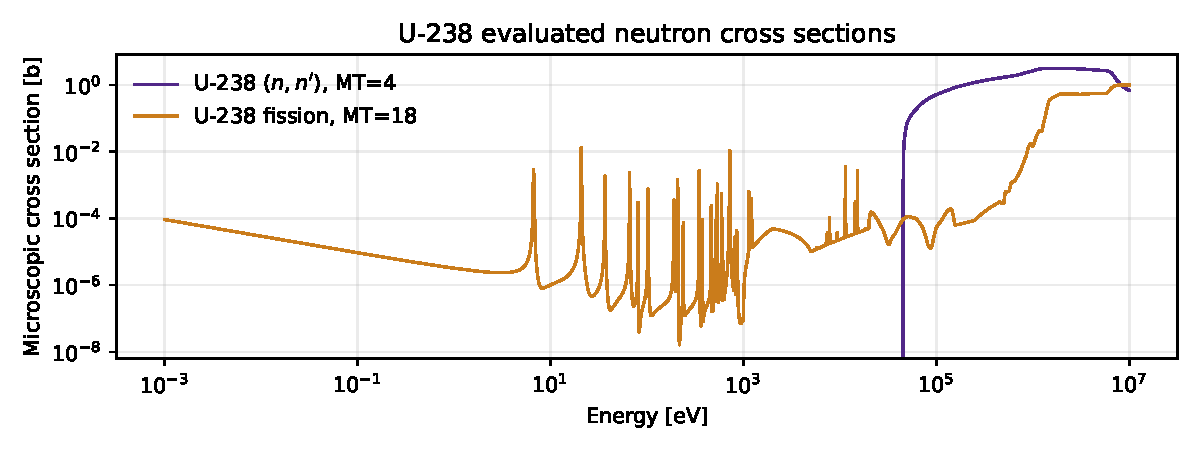
\includegraphics[width=0.98\linewidth]{figures/u238_threshold.pdf}}{\begin{minipage}[t]{0.48\linewidth}
\centering
\fbox{\parbox[c][1.42in][c]{0.91\linewidth}{\centering\sffamily\scriptsize
${}^{238}$U fission\\[4pt]
$\sigma_f(E)$\\[7pt]
\emph{insert threshold-reaction plot}}}
\end{minipage}\hfill
\begin{minipage}[t]{0.48\linewidth}
\centering
\fbox{\parbox[c][1.42in][c]{0.91\linewidth}{\centering\sffamily\scriptsize
${}^{238}$U inelastic\\[4pt]
$\sigma_{in}(E)$\\[7pt]
\emph{insert threshold-reaction plot}}}
\end{minipage}
}
\end{fixedbox}

\begin{boardbox}{What is a threshold telling us?}
For a threshold channel $x$,
\[
\begin{aligned}
 \sigma_x(E)&\approx 0, && E<E_{\mathrm{th}},\\
 \sigma_x(E)&>0,       && E\gtrsim E_{\mathrm{th}}.
\end{aligned}
\]
On the plots, mark $E_{\mathrm{th}}$ and compare how ${}^{238}$U fission and
inelastic scattering turn on.
\RuledLines{4}
\end{boardbox}

\begin{checkpoint}[Connect shape to physics]
A threshold is qualitatively different from a $1/v$ trend because the
reaction channel is \RevealBlank[1.45in]{}.
What physical energy requirement must be met for inelastic scattering?
\RuledLines{2}
\end{checkpoint}

\begin{fixedbox}{Reaction identifiers used in OpenMC}
\scriptsize
\begin{tabularx}{\linewidth}{@{}l c X@{}}
\toprule
$\sigma_{t}$            & 1        & Total cross section \\
$\sigma_{n}$, $\sigma_{e}$ & 2        & Elastic scattering \\
$\sigma_{n'}$, $\sigma_{\mathrm{in}}$ & 4, 51--91 & Inelastic scattering \\
$\sigma_{2n}$           & 16       & $(n,2n)$  \\
$\sigma_{\gamma}$       & 102      & Radiative capture $(n,\gamma)$ \\
$\sigma_{f}$            & 18       & Fission \\
$\sigma_{\alpha}$       & 107      & $(n,\alpha)$ \\
\midrule
$\bar{\nu}$ (total)     & 452      & Average total neutrons per fission \\
$\bar{\nu}_{d}$ (delayed) & 455    & Average delayed neutrons per fission \\
$\bar{\nu}_{p}$ (prompt)  & 456    & Average prompt neutrons per fission \\
\bottomrule
\end{tabularx}
\normalsize
\end{fixedbox}

\end{handoutcolumns}

\newpage
\begin{handoutcolumns}

\HandoutSection{3}{Resonances expose nuclear levels}

\resizebox{\linewidth}{!}{\begin{tikzpicture}[
  x=1cm,
  y=0.72cm,
  >=Latex,
  every node/.style={font=\scriptsize},
  level/.style={line width=0.9pt},
  positive level/.style={level,draw=KSUPurple},
  negative level/.style={level,draw=KSUOrange},
  threshold/.style={line width=0.8pt,densely dashed},
  measure/.style={<->,line width=0.75pt},
  guide/.style={draw=KSUGray,densely dotted}
]

  \draw[threshold] (1.5,0) -- (8.0,0);

  \node[anchor=west,align=left] at (8.15,-0.10)
    {$^{238}\mathrm{U}+n$ threshold\\
     $E_n=0,\quad E_x=S_n$};

  \node[font=\scriptsize\bfseries] at (5.5,3.65)
    {$^{239}\mathrm{U}$ compound-nucleus levels};

  \draw[level] (4.2,-4.4) -- (6.8,-4.4);

  \node[anchor=north,align=center] at (5.5,-4.52)
    {ground state, $E_x=0$};

  \foreach \y in {-3.35,-2.25,-1.05}
    \draw[negative level] (4.2,\y) -- (6.8,\y);

  \node[
    anchor=west,
    align=left,
    text=KSUOrange
  ] at (7.05,-2.20)
    {subthreshold levels\\
     negative resonances\\
     $E_r=E_x-S_n<0$};

  \foreach \y in {0.65,1.30,2.20,3.05}
    \draw[positive level] (4.2,\y) -- (6.8,\y);

  \node[
    anchor=east,
    align=right,
    text=KSUPurple
  ] at (3.90,1.70)
    {positive-energy\\
     resonances, $E_r>0$};

  \draw[measure] (2.55,-4.4) -- (2.55,0);

  \node[anchor=east,align=right] at (2.30,-2.20)
    {neutron binding\\
     (separation) energy\\
     $S_n$};

  \draw[measure] (7.55,0) -- (7.55,2.20);

  \node[anchor=west,align=left] at (7.80,1.10)
    {incident-neutron\\
     kinetic energy $E_n$};

  \draw[measure] (11.25,-4.4) -- (11.25,2.20);

  \node[anchor=west,align=left] at (11.50,-1.10)
    {compound-nucleus\\
     excitation energy\\
     $E_x=S_n+E_n$};

  \draw[guide] (6.8,2.20) -- (11.25,2.20);
  \draw[guide] (6.8,-4.4) -- (11.25,-4.4);

\end{tikzpicture}}

\begin{fixedbox}{${}^{235}$U fission cross section}
\centering
\IfFileExists{figures/u235_fission.pgf}{  \resizebox{0.98\linewidth}{!}{%% Creator: Matplotlib, PGF backend
%%
%% To include the figure in your LaTeX document, write
%%   \input{<filename>.pgf}
%%
%% Make sure the required packages are loaded in your preamble
%%   \usepackage{pgf}
%%
%% Also ensure that all the required font packages are loaded; for instance,
%% the lmodern package is sometimes necessary when using math font.
%%   \usepackage{lmodern}
%%
%% Figures using additional raster images can only be included by \input if
%% they are in the same directory as the main LaTeX file. For loading figures
%% from other directories you can use the `import` package
%%   \usepackage{import}
%%
%% and then include the figures with
%%   \import{<path to file>}{<filename>.pgf}
%%
%% Matplotlib used the following preamble
%%   \def\mathdefault#1{#1}
%%   \everymath=\expandafter{\the\everymath\displaystyle}
%%   \IfFileExists{scrextend.sty}{
%%     \usepackage[fontsize=9.000000pt]{scrextend}
%%   }{
%%     \renewcommand{\normalsize}{\fontsize{9.000000}{10.800000}\selectfont}
%%     \normalsize
%%   }
%%
%%   \makeatletter\@ifpackageloaded{underscore}{}{\usepackage[strings]{underscore}}\makeatother
%%
\begingroup%
\makeatletter%
\begin{pgfpicture}%
\pgfpathrectangle{\pgfpointorigin}{\pgfqpoint{8.000000in}{3.000000in}}%
\pgfusepath{use as bounding box, clip}%
\begin{pgfscope}%
\pgfsetbuttcap%
\pgfsetmiterjoin%
\definecolor{currentfill}{rgb}{1.000000,1.000000,1.000000}%
\pgfsetfillcolor{currentfill}%
\pgfsetlinewidth{0.000000pt}%
\definecolor{currentstroke}{rgb}{1.000000,1.000000,1.000000}%
\pgfsetstrokecolor{currentstroke}%
\pgfsetdash{}{0pt}%
\pgfpathmoveto{\pgfqpoint{0.000000in}{0.000000in}}%
\pgfpathlineto{\pgfqpoint{8.000000in}{0.000000in}}%
\pgfpathlineto{\pgfqpoint{8.000000in}{3.000000in}}%
\pgfpathlineto{\pgfqpoint{0.000000in}{3.000000in}}%
\pgfpathlineto{\pgfqpoint{0.000000in}{0.000000in}}%
\pgfpathclose%
\pgfusepath{fill}%
\end{pgfscope}%
\begin{pgfscope}%
\pgfsetbuttcap%
\pgfsetmiterjoin%
\definecolor{currentfill}{rgb}{1.000000,1.000000,1.000000}%
\pgfsetfillcolor{currentfill}%
\pgfsetlinewidth{0.000000pt}%
\definecolor{currentstroke}{rgb}{0.000000,0.000000,0.000000}%
\pgfsetstrokecolor{currentstroke}%
\pgfsetstrokeopacity{0.000000}%
\pgfsetdash{}{0pt}%
\pgfpathmoveto{\pgfqpoint{0.589925in}{0.540552in}}%
\pgfpathlineto{\pgfqpoint{7.865000in}{0.540552in}}%
\pgfpathlineto{\pgfqpoint{7.865000in}{2.661666in}}%
\pgfpathlineto{\pgfqpoint{0.589925in}{2.661666in}}%
\pgfpathlineto{\pgfqpoint{0.589925in}{0.540552in}}%
\pgfpathclose%
\pgfusepath{fill}%
\end{pgfscope}%
\begin{pgfscope}%
\pgfsetbuttcap%
\pgfsetroundjoin%
\definecolor{currentfill}{rgb}{0.000000,0.000000,0.000000}%
\pgfsetfillcolor{currentfill}%
\pgfsetlinewidth{0.803000pt}%
\definecolor{currentstroke}{rgb}{0.000000,0.000000,0.000000}%
\pgfsetstrokecolor{currentstroke}%
\pgfsetdash{}{0pt}%
\pgfsys@defobject{currentmarker}{\pgfqpoint{0.000000in}{-0.048611in}}{\pgfqpoint{0.000000in}{0.000000in}}{%
\pgfpathmoveto{\pgfqpoint{0.000000in}{0.000000in}}%
\pgfpathlineto{\pgfqpoint{0.000000in}{-0.048611in}}%
\pgfusepath{stroke,fill}%
}%
\begin{pgfscope}%
\pgfsys@transformshift{0.920611in}{0.540552in}%
\pgfsys@useobject{currentmarker}{}%
\end{pgfscope}%
\end{pgfscope}%
\begin{pgfscope}%
\definecolor{textcolor}{rgb}{0.000000,0.000000,0.000000}%
\pgfsetstrokecolor{textcolor}%
\pgfsetfillcolor{textcolor}%
\pgftext[x=0.920611in,y=0.443330in,,top]{\color{textcolor}{\rmfamily\fontsize{8.000000}{9.600000}\selectfont\catcode`\^=\active\def^{\ifmmode\sp\else\^{}\fi}\catcode`\%=\active\def%{\%}$\mathdefault{10^{-2}}$}}%
\end{pgfscope}%
\begin{pgfscope}%
\pgfsetbuttcap%
\pgfsetroundjoin%
\definecolor{currentfill}{rgb}{0.000000,0.000000,0.000000}%
\pgfsetfillcolor{currentfill}%
\pgfsetlinewidth{0.803000pt}%
\definecolor{currentstroke}{rgb}{0.000000,0.000000,0.000000}%
\pgfsetstrokecolor{currentstroke}%
\pgfsetdash{}{0pt}%
\pgfsys@defobject{currentmarker}{\pgfqpoint{0.000000in}{-0.048611in}}{\pgfqpoint{0.000000in}{0.000000in}}{%
\pgfpathmoveto{\pgfqpoint{0.000000in}{0.000000in}}%
\pgfpathlineto{\pgfqpoint{0.000000in}{-0.048611in}}%
\pgfusepath{stroke,fill}%
}%
\begin{pgfscope}%
\pgfsys@transformshift{2.390323in}{0.540552in}%
\pgfsys@useobject{currentmarker}{}%
\end{pgfscope}%
\end{pgfscope}%
\begin{pgfscope}%
\definecolor{textcolor}{rgb}{0.000000,0.000000,0.000000}%
\pgfsetstrokecolor{textcolor}%
\pgfsetfillcolor{textcolor}%
\pgftext[x=2.390323in,y=0.443330in,,top]{\color{textcolor}{\rmfamily\fontsize{8.000000}{9.600000}\selectfont\catcode`\^=\active\def^{\ifmmode\sp\else\^{}\fi}\catcode`\%=\active\def%{\%}$\mathdefault{10^{0}}$}}%
\end{pgfscope}%
\begin{pgfscope}%
\pgfsetbuttcap%
\pgfsetroundjoin%
\definecolor{currentfill}{rgb}{0.000000,0.000000,0.000000}%
\pgfsetfillcolor{currentfill}%
\pgfsetlinewidth{0.803000pt}%
\definecolor{currentstroke}{rgb}{0.000000,0.000000,0.000000}%
\pgfsetstrokecolor{currentstroke}%
\pgfsetdash{}{0pt}%
\pgfsys@defobject{currentmarker}{\pgfqpoint{0.000000in}{-0.048611in}}{\pgfqpoint{0.000000in}{0.000000in}}{%
\pgfpathmoveto{\pgfqpoint{0.000000in}{0.000000in}}%
\pgfpathlineto{\pgfqpoint{0.000000in}{-0.048611in}}%
\pgfusepath{stroke,fill}%
}%
\begin{pgfscope}%
\pgfsys@transformshift{3.860035in}{0.540552in}%
\pgfsys@useobject{currentmarker}{}%
\end{pgfscope}%
\end{pgfscope}%
\begin{pgfscope}%
\definecolor{textcolor}{rgb}{0.000000,0.000000,0.000000}%
\pgfsetstrokecolor{textcolor}%
\pgfsetfillcolor{textcolor}%
\pgftext[x=3.860035in,y=0.443330in,,top]{\color{textcolor}{\rmfamily\fontsize{8.000000}{9.600000}\selectfont\catcode`\^=\active\def^{\ifmmode\sp\else\^{}\fi}\catcode`\%=\active\def%{\%}$\mathdefault{10^{2}}$}}%
\end{pgfscope}%
\begin{pgfscope}%
\pgfsetbuttcap%
\pgfsetroundjoin%
\definecolor{currentfill}{rgb}{0.000000,0.000000,0.000000}%
\pgfsetfillcolor{currentfill}%
\pgfsetlinewidth{0.803000pt}%
\definecolor{currentstroke}{rgb}{0.000000,0.000000,0.000000}%
\pgfsetstrokecolor{currentstroke}%
\pgfsetdash{}{0pt}%
\pgfsys@defobject{currentmarker}{\pgfqpoint{0.000000in}{-0.048611in}}{\pgfqpoint{0.000000in}{0.000000in}}{%
\pgfpathmoveto{\pgfqpoint{0.000000in}{0.000000in}}%
\pgfpathlineto{\pgfqpoint{0.000000in}{-0.048611in}}%
\pgfusepath{stroke,fill}%
}%
\begin{pgfscope}%
\pgfsys@transformshift{5.329747in}{0.540552in}%
\pgfsys@useobject{currentmarker}{}%
\end{pgfscope}%
\end{pgfscope}%
\begin{pgfscope}%
\definecolor{textcolor}{rgb}{0.000000,0.000000,0.000000}%
\pgfsetstrokecolor{textcolor}%
\pgfsetfillcolor{textcolor}%
\pgftext[x=5.329747in,y=0.443330in,,top]{\color{textcolor}{\rmfamily\fontsize{8.000000}{9.600000}\selectfont\catcode`\^=\active\def^{\ifmmode\sp\else\^{}\fi}\catcode`\%=\active\def%{\%}$\mathdefault{10^{4}}$}}%
\end{pgfscope}%
\begin{pgfscope}%
\pgfsetbuttcap%
\pgfsetroundjoin%
\definecolor{currentfill}{rgb}{0.000000,0.000000,0.000000}%
\pgfsetfillcolor{currentfill}%
\pgfsetlinewidth{0.803000pt}%
\definecolor{currentstroke}{rgb}{0.000000,0.000000,0.000000}%
\pgfsetstrokecolor{currentstroke}%
\pgfsetdash{}{0pt}%
\pgfsys@defobject{currentmarker}{\pgfqpoint{0.000000in}{-0.048611in}}{\pgfqpoint{0.000000in}{0.000000in}}{%
\pgfpathmoveto{\pgfqpoint{0.000000in}{0.000000in}}%
\pgfpathlineto{\pgfqpoint{0.000000in}{-0.048611in}}%
\pgfusepath{stroke,fill}%
}%
\begin{pgfscope}%
\pgfsys@transformshift{6.799459in}{0.540552in}%
\pgfsys@useobject{currentmarker}{}%
\end{pgfscope}%
\end{pgfscope}%
\begin{pgfscope}%
\definecolor{textcolor}{rgb}{0.000000,0.000000,0.000000}%
\pgfsetstrokecolor{textcolor}%
\pgfsetfillcolor{textcolor}%
\pgftext[x=6.799459in,y=0.443330in,,top]{\color{textcolor}{\rmfamily\fontsize{8.000000}{9.600000}\selectfont\catcode`\^=\active\def^{\ifmmode\sp\else\^{}\fi}\catcode`\%=\active\def%{\%}$\mathdefault{10^{6}}$}}%
\end{pgfscope}%
\begin{pgfscope}%
\definecolor{textcolor}{rgb}{0.000000,0.000000,0.000000}%
\pgfsetstrokecolor{textcolor}%
\pgfsetfillcolor{textcolor}%
\pgftext[x=4.227463in,y=0.261221in,,top]{\color{textcolor}{\rmfamily\fontsize{9.000000}{10.800000}\selectfont\catcode`\^=\active\def^{\ifmmode\sp\else\^{}\fi}\catcode`\%=\active\def%{\%}$E$ (eV)}}%
\end{pgfscope}%
\begin{pgfscope}%
\pgfsetbuttcap%
\pgfsetroundjoin%
\definecolor{currentfill}{rgb}{0.000000,0.000000,0.000000}%
\pgfsetfillcolor{currentfill}%
\pgfsetlinewidth{0.803000pt}%
\definecolor{currentstroke}{rgb}{0.000000,0.000000,0.000000}%
\pgfsetstrokecolor{currentstroke}%
\pgfsetdash{}{0pt}%
\pgfsys@defobject{currentmarker}{\pgfqpoint{-0.048611in}{0.000000in}}{\pgfqpoint{-0.000000in}{0.000000in}}{%
\pgfpathmoveto{\pgfqpoint{-0.000000in}{0.000000in}}%
\pgfpathlineto{\pgfqpoint{-0.048611in}{0.000000in}}%
\pgfusepath{stroke,fill}%
}%
\begin{pgfscope}%
\pgfsys@transformshift{0.589925in}{0.765440in}%
\pgfsys@useobject{currentmarker}{}%
\end{pgfscope}%
\end{pgfscope}%
\begin{pgfscope}%
\definecolor{textcolor}{rgb}{0.000000,0.000000,0.000000}%
\pgfsetstrokecolor{textcolor}%
\pgfsetfillcolor{textcolor}%
\pgftext[x=0.316776in, y=0.715510in, left, base]{\color{textcolor}{\rmfamily\fontsize{8.000000}{9.600000}\selectfont\catcode`\^=\active\def^{\ifmmode\sp\else\^{}\fi}\catcode`\%=\active\def%{\%}$\mathdefault{10^{0}}$}}%
\end{pgfscope}%
\begin{pgfscope}%
\pgfsetbuttcap%
\pgfsetroundjoin%
\definecolor{currentfill}{rgb}{0.000000,0.000000,0.000000}%
\pgfsetfillcolor{currentfill}%
\pgfsetlinewidth{0.803000pt}%
\definecolor{currentstroke}{rgb}{0.000000,0.000000,0.000000}%
\pgfsetstrokecolor{currentstroke}%
\pgfsetdash{}{0pt}%
\pgfsys@defobject{currentmarker}{\pgfqpoint{-0.048611in}{0.000000in}}{\pgfqpoint{-0.000000in}{0.000000in}}{%
\pgfpathmoveto{\pgfqpoint{-0.000000in}{0.000000in}}%
\pgfpathlineto{\pgfqpoint{-0.048611in}{0.000000in}}%
\pgfusepath{stroke,fill}%
}%
\begin{pgfscope}%
\pgfsys@transformshift{0.589925in}{1.369459in}%
\pgfsys@useobject{currentmarker}{}%
\end{pgfscope}%
\end{pgfscope}%
\begin{pgfscope}%
\definecolor{textcolor}{rgb}{0.000000,0.000000,0.000000}%
\pgfsetstrokecolor{textcolor}%
\pgfsetfillcolor{textcolor}%
\pgftext[x=0.316776in, y=1.319529in, left, base]{\color{textcolor}{\rmfamily\fontsize{8.000000}{9.600000}\selectfont\catcode`\^=\active\def^{\ifmmode\sp\else\^{}\fi}\catcode`\%=\active\def%{\%}$\mathdefault{10^{1}}$}}%
\end{pgfscope}%
\begin{pgfscope}%
\pgfsetbuttcap%
\pgfsetroundjoin%
\definecolor{currentfill}{rgb}{0.000000,0.000000,0.000000}%
\pgfsetfillcolor{currentfill}%
\pgfsetlinewidth{0.803000pt}%
\definecolor{currentstroke}{rgb}{0.000000,0.000000,0.000000}%
\pgfsetstrokecolor{currentstroke}%
\pgfsetdash{}{0pt}%
\pgfsys@defobject{currentmarker}{\pgfqpoint{-0.048611in}{0.000000in}}{\pgfqpoint{-0.000000in}{0.000000in}}{%
\pgfpathmoveto{\pgfqpoint{-0.000000in}{0.000000in}}%
\pgfpathlineto{\pgfqpoint{-0.048611in}{0.000000in}}%
\pgfusepath{stroke,fill}%
}%
\begin{pgfscope}%
\pgfsys@transformshift{0.589925in}{1.973478in}%
\pgfsys@useobject{currentmarker}{}%
\end{pgfscope}%
\end{pgfscope}%
\begin{pgfscope}%
\definecolor{textcolor}{rgb}{0.000000,0.000000,0.000000}%
\pgfsetstrokecolor{textcolor}%
\pgfsetfillcolor{textcolor}%
\pgftext[x=0.316776in, y=1.923547in, left, base]{\color{textcolor}{\rmfamily\fontsize{8.000000}{9.600000}\selectfont\catcode`\^=\active\def^{\ifmmode\sp\else\^{}\fi}\catcode`\%=\active\def%{\%}$\mathdefault{10^{2}}$}}%
\end{pgfscope}%
\begin{pgfscope}%
\pgfsetbuttcap%
\pgfsetroundjoin%
\definecolor{currentfill}{rgb}{0.000000,0.000000,0.000000}%
\pgfsetfillcolor{currentfill}%
\pgfsetlinewidth{0.803000pt}%
\definecolor{currentstroke}{rgb}{0.000000,0.000000,0.000000}%
\pgfsetstrokecolor{currentstroke}%
\pgfsetdash{}{0pt}%
\pgfsys@defobject{currentmarker}{\pgfqpoint{-0.048611in}{0.000000in}}{\pgfqpoint{-0.000000in}{0.000000in}}{%
\pgfpathmoveto{\pgfqpoint{-0.000000in}{0.000000in}}%
\pgfpathlineto{\pgfqpoint{-0.048611in}{0.000000in}}%
\pgfusepath{stroke,fill}%
}%
\begin{pgfscope}%
\pgfsys@transformshift{0.589925in}{2.577497in}%
\pgfsys@useobject{currentmarker}{}%
\end{pgfscope}%
\end{pgfscope}%
\begin{pgfscope}%
\definecolor{textcolor}{rgb}{0.000000,0.000000,0.000000}%
\pgfsetstrokecolor{textcolor}%
\pgfsetfillcolor{textcolor}%
\pgftext[x=0.316776in, y=2.527566in, left, base]{\color{textcolor}{\rmfamily\fontsize{8.000000}{9.600000}\selectfont\catcode`\^=\active\def^{\ifmmode\sp\else\^{}\fi}\catcode`\%=\active\def%{\%}$\mathdefault{10^{3}}$}}%
\end{pgfscope}%
\begin{pgfscope}%
\pgfsetbuttcap%
\pgfsetroundjoin%
\definecolor{currentfill}{rgb}{0.000000,0.000000,0.000000}%
\pgfsetfillcolor{currentfill}%
\pgfsetlinewidth{0.602250pt}%
\definecolor{currentstroke}{rgb}{0.000000,0.000000,0.000000}%
\pgfsetstrokecolor{currentstroke}%
\pgfsetdash{}{0pt}%
\pgfsys@defobject{currentmarker}{\pgfqpoint{-0.027778in}{0.000000in}}{\pgfqpoint{-0.000000in}{0.000000in}}{%
\pgfpathmoveto{\pgfqpoint{-0.000000in}{0.000000in}}%
\pgfpathlineto{\pgfqpoint{-0.027778in}{0.000000in}}%
\pgfusepath{stroke,fill}%
}%
\begin{pgfscope}%
\pgfsys@transformshift{0.589925in}{0.583613in}%
\pgfsys@useobject{currentmarker}{}%
\end{pgfscope}%
\end{pgfscope}%
\begin{pgfscope}%
\pgfsetbuttcap%
\pgfsetroundjoin%
\definecolor{currentfill}{rgb}{0.000000,0.000000,0.000000}%
\pgfsetfillcolor{currentfill}%
\pgfsetlinewidth{0.602250pt}%
\definecolor{currentstroke}{rgb}{0.000000,0.000000,0.000000}%
\pgfsetstrokecolor{currentstroke}%
\pgfsetdash{}{0pt}%
\pgfsys@defobject{currentmarker}{\pgfqpoint{-0.027778in}{0.000000in}}{\pgfqpoint{-0.000000in}{0.000000in}}{%
\pgfpathmoveto{\pgfqpoint{-0.000000in}{0.000000in}}%
\pgfpathlineto{\pgfqpoint{-0.027778in}{0.000000in}}%
\pgfusepath{stroke,fill}%
}%
\begin{pgfscope}%
\pgfsys@transformshift{0.589925in}{0.631440in}%
\pgfsys@useobject{currentmarker}{}%
\end{pgfscope}%
\end{pgfscope}%
\begin{pgfscope}%
\pgfsetbuttcap%
\pgfsetroundjoin%
\definecolor{currentfill}{rgb}{0.000000,0.000000,0.000000}%
\pgfsetfillcolor{currentfill}%
\pgfsetlinewidth{0.602250pt}%
\definecolor{currentstroke}{rgb}{0.000000,0.000000,0.000000}%
\pgfsetstrokecolor{currentstroke}%
\pgfsetdash{}{0pt}%
\pgfsys@defobject{currentmarker}{\pgfqpoint{-0.027778in}{0.000000in}}{\pgfqpoint{-0.000000in}{0.000000in}}{%
\pgfpathmoveto{\pgfqpoint{-0.000000in}{0.000000in}}%
\pgfpathlineto{\pgfqpoint{-0.027778in}{0.000000in}}%
\pgfusepath{stroke,fill}%
}%
\begin{pgfscope}%
\pgfsys@transformshift{0.589925in}{0.671877in}%
\pgfsys@useobject{currentmarker}{}%
\end{pgfscope}%
\end{pgfscope}%
\begin{pgfscope}%
\pgfsetbuttcap%
\pgfsetroundjoin%
\definecolor{currentfill}{rgb}{0.000000,0.000000,0.000000}%
\pgfsetfillcolor{currentfill}%
\pgfsetlinewidth{0.602250pt}%
\definecolor{currentstroke}{rgb}{0.000000,0.000000,0.000000}%
\pgfsetstrokecolor{currentstroke}%
\pgfsetdash{}{0pt}%
\pgfsys@defobject{currentmarker}{\pgfqpoint{-0.027778in}{0.000000in}}{\pgfqpoint{-0.000000in}{0.000000in}}{%
\pgfpathmoveto{\pgfqpoint{-0.000000in}{0.000000in}}%
\pgfpathlineto{\pgfqpoint{-0.027778in}{0.000000in}}%
\pgfusepath{stroke,fill}%
}%
\begin{pgfscope}%
\pgfsys@transformshift{0.589925in}{0.706905in}%
\pgfsys@useobject{currentmarker}{}%
\end{pgfscope}%
\end{pgfscope}%
\begin{pgfscope}%
\pgfsetbuttcap%
\pgfsetroundjoin%
\definecolor{currentfill}{rgb}{0.000000,0.000000,0.000000}%
\pgfsetfillcolor{currentfill}%
\pgfsetlinewidth{0.602250pt}%
\definecolor{currentstroke}{rgb}{0.000000,0.000000,0.000000}%
\pgfsetstrokecolor{currentstroke}%
\pgfsetdash{}{0pt}%
\pgfsys@defobject{currentmarker}{\pgfqpoint{-0.027778in}{0.000000in}}{\pgfqpoint{-0.000000in}{0.000000in}}{%
\pgfpathmoveto{\pgfqpoint{-0.000000in}{0.000000in}}%
\pgfpathlineto{\pgfqpoint{-0.027778in}{0.000000in}}%
\pgfusepath{stroke,fill}%
}%
\begin{pgfscope}%
\pgfsys@transformshift{0.589925in}{0.737802in}%
\pgfsys@useobject{currentmarker}{}%
\end{pgfscope}%
\end{pgfscope}%
\begin{pgfscope}%
\pgfsetbuttcap%
\pgfsetroundjoin%
\definecolor{currentfill}{rgb}{0.000000,0.000000,0.000000}%
\pgfsetfillcolor{currentfill}%
\pgfsetlinewidth{0.602250pt}%
\definecolor{currentstroke}{rgb}{0.000000,0.000000,0.000000}%
\pgfsetstrokecolor{currentstroke}%
\pgfsetdash{}{0pt}%
\pgfsys@defobject{currentmarker}{\pgfqpoint{-0.027778in}{0.000000in}}{\pgfqpoint{-0.000000in}{0.000000in}}{%
\pgfpathmoveto{\pgfqpoint{-0.000000in}{0.000000in}}%
\pgfpathlineto{\pgfqpoint{-0.027778in}{0.000000in}}%
\pgfusepath{stroke,fill}%
}%
\begin{pgfscope}%
\pgfsys@transformshift{0.589925in}{0.947268in}%
\pgfsys@useobject{currentmarker}{}%
\end{pgfscope}%
\end{pgfscope}%
\begin{pgfscope}%
\pgfsetbuttcap%
\pgfsetroundjoin%
\definecolor{currentfill}{rgb}{0.000000,0.000000,0.000000}%
\pgfsetfillcolor{currentfill}%
\pgfsetlinewidth{0.602250pt}%
\definecolor{currentstroke}{rgb}{0.000000,0.000000,0.000000}%
\pgfsetstrokecolor{currentstroke}%
\pgfsetdash{}{0pt}%
\pgfsys@defobject{currentmarker}{\pgfqpoint{-0.027778in}{0.000000in}}{\pgfqpoint{-0.000000in}{0.000000in}}{%
\pgfpathmoveto{\pgfqpoint{-0.000000in}{0.000000in}}%
\pgfpathlineto{\pgfqpoint{-0.027778in}{0.000000in}}%
\pgfusepath{stroke,fill}%
}%
\begin{pgfscope}%
\pgfsys@transformshift{0.589925in}{1.053631in}%
\pgfsys@useobject{currentmarker}{}%
\end{pgfscope}%
\end{pgfscope}%
\begin{pgfscope}%
\pgfsetbuttcap%
\pgfsetroundjoin%
\definecolor{currentfill}{rgb}{0.000000,0.000000,0.000000}%
\pgfsetfillcolor{currentfill}%
\pgfsetlinewidth{0.602250pt}%
\definecolor{currentstroke}{rgb}{0.000000,0.000000,0.000000}%
\pgfsetstrokecolor{currentstroke}%
\pgfsetdash{}{0pt}%
\pgfsys@defobject{currentmarker}{\pgfqpoint{-0.027778in}{0.000000in}}{\pgfqpoint{-0.000000in}{0.000000in}}{%
\pgfpathmoveto{\pgfqpoint{-0.000000in}{0.000000in}}%
\pgfpathlineto{\pgfqpoint{-0.027778in}{0.000000in}}%
\pgfusepath{stroke,fill}%
}%
\begin{pgfscope}%
\pgfsys@transformshift{0.589925in}{1.129096in}%
\pgfsys@useobject{currentmarker}{}%
\end{pgfscope}%
\end{pgfscope}%
\begin{pgfscope}%
\pgfsetbuttcap%
\pgfsetroundjoin%
\definecolor{currentfill}{rgb}{0.000000,0.000000,0.000000}%
\pgfsetfillcolor{currentfill}%
\pgfsetlinewidth{0.602250pt}%
\definecolor{currentstroke}{rgb}{0.000000,0.000000,0.000000}%
\pgfsetstrokecolor{currentstroke}%
\pgfsetdash{}{0pt}%
\pgfsys@defobject{currentmarker}{\pgfqpoint{-0.027778in}{0.000000in}}{\pgfqpoint{-0.000000in}{0.000000in}}{%
\pgfpathmoveto{\pgfqpoint{-0.000000in}{0.000000in}}%
\pgfpathlineto{\pgfqpoint{-0.027778in}{0.000000in}}%
\pgfusepath{stroke,fill}%
}%
\begin{pgfscope}%
\pgfsys@transformshift{0.589925in}{1.187631in}%
\pgfsys@useobject{currentmarker}{}%
\end{pgfscope}%
\end{pgfscope}%
\begin{pgfscope}%
\pgfsetbuttcap%
\pgfsetroundjoin%
\definecolor{currentfill}{rgb}{0.000000,0.000000,0.000000}%
\pgfsetfillcolor{currentfill}%
\pgfsetlinewidth{0.602250pt}%
\definecolor{currentstroke}{rgb}{0.000000,0.000000,0.000000}%
\pgfsetstrokecolor{currentstroke}%
\pgfsetdash{}{0pt}%
\pgfsys@defobject{currentmarker}{\pgfqpoint{-0.027778in}{0.000000in}}{\pgfqpoint{-0.000000in}{0.000000in}}{%
\pgfpathmoveto{\pgfqpoint{-0.000000in}{0.000000in}}%
\pgfpathlineto{\pgfqpoint{-0.027778in}{0.000000in}}%
\pgfusepath{stroke,fill}%
}%
\begin{pgfscope}%
\pgfsys@transformshift{0.589925in}{1.235458in}%
\pgfsys@useobject{currentmarker}{}%
\end{pgfscope}%
\end{pgfscope}%
\begin{pgfscope}%
\pgfsetbuttcap%
\pgfsetroundjoin%
\definecolor{currentfill}{rgb}{0.000000,0.000000,0.000000}%
\pgfsetfillcolor{currentfill}%
\pgfsetlinewidth{0.602250pt}%
\definecolor{currentstroke}{rgb}{0.000000,0.000000,0.000000}%
\pgfsetstrokecolor{currentstroke}%
\pgfsetdash{}{0pt}%
\pgfsys@defobject{currentmarker}{\pgfqpoint{-0.027778in}{0.000000in}}{\pgfqpoint{-0.000000in}{0.000000in}}{%
\pgfpathmoveto{\pgfqpoint{-0.000000in}{0.000000in}}%
\pgfpathlineto{\pgfqpoint{-0.027778in}{0.000000in}}%
\pgfusepath{stroke,fill}%
}%
\begin{pgfscope}%
\pgfsys@transformshift{0.589925in}{1.275895in}%
\pgfsys@useobject{currentmarker}{}%
\end{pgfscope}%
\end{pgfscope}%
\begin{pgfscope}%
\pgfsetbuttcap%
\pgfsetroundjoin%
\definecolor{currentfill}{rgb}{0.000000,0.000000,0.000000}%
\pgfsetfillcolor{currentfill}%
\pgfsetlinewidth{0.602250pt}%
\definecolor{currentstroke}{rgb}{0.000000,0.000000,0.000000}%
\pgfsetstrokecolor{currentstroke}%
\pgfsetdash{}{0pt}%
\pgfsys@defobject{currentmarker}{\pgfqpoint{-0.027778in}{0.000000in}}{\pgfqpoint{-0.000000in}{0.000000in}}{%
\pgfpathmoveto{\pgfqpoint{-0.000000in}{0.000000in}}%
\pgfpathlineto{\pgfqpoint{-0.027778in}{0.000000in}}%
\pgfusepath{stroke,fill}%
}%
\begin{pgfscope}%
\pgfsys@transformshift{0.589925in}{1.310924in}%
\pgfsys@useobject{currentmarker}{}%
\end{pgfscope}%
\end{pgfscope}%
\begin{pgfscope}%
\pgfsetbuttcap%
\pgfsetroundjoin%
\definecolor{currentfill}{rgb}{0.000000,0.000000,0.000000}%
\pgfsetfillcolor{currentfill}%
\pgfsetlinewidth{0.602250pt}%
\definecolor{currentstroke}{rgb}{0.000000,0.000000,0.000000}%
\pgfsetstrokecolor{currentstroke}%
\pgfsetdash{}{0pt}%
\pgfsys@defobject{currentmarker}{\pgfqpoint{-0.027778in}{0.000000in}}{\pgfqpoint{-0.000000in}{0.000000in}}{%
\pgfpathmoveto{\pgfqpoint{-0.000000in}{0.000000in}}%
\pgfpathlineto{\pgfqpoint{-0.027778in}{0.000000in}}%
\pgfusepath{stroke,fill}%
}%
\begin{pgfscope}%
\pgfsys@transformshift{0.589925in}{1.341821in}%
\pgfsys@useobject{currentmarker}{}%
\end{pgfscope}%
\end{pgfscope}%
\begin{pgfscope}%
\pgfsetbuttcap%
\pgfsetroundjoin%
\definecolor{currentfill}{rgb}{0.000000,0.000000,0.000000}%
\pgfsetfillcolor{currentfill}%
\pgfsetlinewidth{0.602250pt}%
\definecolor{currentstroke}{rgb}{0.000000,0.000000,0.000000}%
\pgfsetstrokecolor{currentstroke}%
\pgfsetdash{}{0pt}%
\pgfsys@defobject{currentmarker}{\pgfqpoint{-0.027778in}{0.000000in}}{\pgfqpoint{-0.000000in}{0.000000in}}{%
\pgfpathmoveto{\pgfqpoint{-0.000000in}{0.000000in}}%
\pgfpathlineto{\pgfqpoint{-0.027778in}{0.000000in}}%
\pgfusepath{stroke,fill}%
}%
\begin{pgfscope}%
\pgfsys@transformshift{0.589925in}{1.551287in}%
\pgfsys@useobject{currentmarker}{}%
\end{pgfscope}%
\end{pgfscope}%
\begin{pgfscope}%
\pgfsetbuttcap%
\pgfsetroundjoin%
\definecolor{currentfill}{rgb}{0.000000,0.000000,0.000000}%
\pgfsetfillcolor{currentfill}%
\pgfsetlinewidth{0.602250pt}%
\definecolor{currentstroke}{rgb}{0.000000,0.000000,0.000000}%
\pgfsetstrokecolor{currentstroke}%
\pgfsetdash{}{0pt}%
\pgfsys@defobject{currentmarker}{\pgfqpoint{-0.027778in}{0.000000in}}{\pgfqpoint{-0.000000in}{0.000000in}}{%
\pgfpathmoveto{\pgfqpoint{-0.000000in}{0.000000in}}%
\pgfpathlineto{\pgfqpoint{-0.027778in}{0.000000in}}%
\pgfusepath{stroke,fill}%
}%
\begin{pgfscope}%
\pgfsys@transformshift{0.589925in}{1.657649in}%
\pgfsys@useobject{currentmarker}{}%
\end{pgfscope}%
\end{pgfscope}%
\begin{pgfscope}%
\pgfsetbuttcap%
\pgfsetroundjoin%
\definecolor{currentfill}{rgb}{0.000000,0.000000,0.000000}%
\pgfsetfillcolor{currentfill}%
\pgfsetlinewidth{0.602250pt}%
\definecolor{currentstroke}{rgb}{0.000000,0.000000,0.000000}%
\pgfsetstrokecolor{currentstroke}%
\pgfsetdash{}{0pt}%
\pgfsys@defobject{currentmarker}{\pgfqpoint{-0.027778in}{0.000000in}}{\pgfqpoint{-0.000000in}{0.000000in}}{%
\pgfpathmoveto{\pgfqpoint{-0.000000in}{0.000000in}}%
\pgfpathlineto{\pgfqpoint{-0.027778in}{0.000000in}}%
\pgfusepath{stroke,fill}%
}%
\begin{pgfscope}%
\pgfsys@transformshift{0.589925in}{1.733115in}%
\pgfsys@useobject{currentmarker}{}%
\end{pgfscope}%
\end{pgfscope}%
\begin{pgfscope}%
\pgfsetbuttcap%
\pgfsetroundjoin%
\definecolor{currentfill}{rgb}{0.000000,0.000000,0.000000}%
\pgfsetfillcolor{currentfill}%
\pgfsetlinewidth{0.602250pt}%
\definecolor{currentstroke}{rgb}{0.000000,0.000000,0.000000}%
\pgfsetstrokecolor{currentstroke}%
\pgfsetdash{}{0pt}%
\pgfsys@defobject{currentmarker}{\pgfqpoint{-0.027778in}{0.000000in}}{\pgfqpoint{-0.000000in}{0.000000in}}{%
\pgfpathmoveto{\pgfqpoint{-0.000000in}{0.000000in}}%
\pgfpathlineto{\pgfqpoint{-0.027778in}{0.000000in}}%
\pgfusepath{stroke,fill}%
}%
\begin{pgfscope}%
\pgfsys@transformshift{0.589925in}{1.791650in}%
\pgfsys@useobject{currentmarker}{}%
\end{pgfscope}%
\end{pgfscope}%
\begin{pgfscope}%
\pgfsetbuttcap%
\pgfsetroundjoin%
\definecolor{currentfill}{rgb}{0.000000,0.000000,0.000000}%
\pgfsetfillcolor{currentfill}%
\pgfsetlinewidth{0.602250pt}%
\definecolor{currentstroke}{rgb}{0.000000,0.000000,0.000000}%
\pgfsetstrokecolor{currentstroke}%
\pgfsetdash{}{0pt}%
\pgfsys@defobject{currentmarker}{\pgfqpoint{-0.027778in}{0.000000in}}{\pgfqpoint{-0.000000in}{0.000000in}}{%
\pgfpathmoveto{\pgfqpoint{-0.000000in}{0.000000in}}%
\pgfpathlineto{\pgfqpoint{-0.027778in}{0.000000in}}%
\pgfusepath{stroke,fill}%
}%
\begin{pgfscope}%
\pgfsys@transformshift{0.589925in}{1.839477in}%
\pgfsys@useobject{currentmarker}{}%
\end{pgfscope}%
\end{pgfscope}%
\begin{pgfscope}%
\pgfsetbuttcap%
\pgfsetroundjoin%
\definecolor{currentfill}{rgb}{0.000000,0.000000,0.000000}%
\pgfsetfillcolor{currentfill}%
\pgfsetlinewidth{0.602250pt}%
\definecolor{currentstroke}{rgb}{0.000000,0.000000,0.000000}%
\pgfsetstrokecolor{currentstroke}%
\pgfsetdash{}{0pt}%
\pgfsys@defobject{currentmarker}{\pgfqpoint{-0.027778in}{0.000000in}}{\pgfqpoint{-0.000000in}{0.000000in}}{%
\pgfpathmoveto{\pgfqpoint{-0.000000in}{0.000000in}}%
\pgfpathlineto{\pgfqpoint{-0.027778in}{0.000000in}}%
\pgfusepath{stroke,fill}%
}%
\begin{pgfscope}%
\pgfsys@transformshift{0.589925in}{1.879914in}%
\pgfsys@useobject{currentmarker}{}%
\end{pgfscope}%
\end{pgfscope}%
\begin{pgfscope}%
\pgfsetbuttcap%
\pgfsetroundjoin%
\definecolor{currentfill}{rgb}{0.000000,0.000000,0.000000}%
\pgfsetfillcolor{currentfill}%
\pgfsetlinewidth{0.602250pt}%
\definecolor{currentstroke}{rgb}{0.000000,0.000000,0.000000}%
\pgfsetstrokecolor{currentstroke}%
\pgfsetdash{}{0pt}%
\pgfsys@defobject{currentmarker}{\pgfqpoint{-0.027778in}{0.000000in}}{\pgfqpoint{-0.000000in}{0.000000in}}{%
\pgfpathmoveto{\pgfqpoint{-0.000000in}{0.000000in}}%
\pgfpathlineto{\pgfqpoint{-0.027778in}{0.000000in}}%
\pgfusepath{stroke,fill}%
}%
\begin{pgfscope}%
\pgfsys@transformshift{0.589925in}{1.914942in}%
\pgfsys@useobject{currentmarker}{}%
\end{pgfscope}%
\end{pgfscope}%
\begin{pgfscope}%
\pgfsetbuttcap%
\pgfsetroundjoin%
\definecolor{currentfill}{rgb}{0.000000,0.000000,0.000000}%
\pgfsetfillcolor{currentfill}%
\pgfsetlinewidth{0.602250pt}%
\definecolor{currentstroke}{rgb}{0.000000,0.000000,0.000000}%
\pgfsetstrokecolor{currentstroke}%
\pgfsetdash{}{0pt}%
\pgfsys@defobject{currentmarker}{\pgfqpoint{-0.027778in}{0.000000in}}{\pgfqpoint{-0.000000in}{0.000000in}}{%
\pgfpathmoveto{\pgfqpoint{-0.000000in}{0.000000in}}%
\pgfpathlineto{\pgfqpoint{-0.027778in}{0.000000in}}%
\pgfusepath{stroke,fill}%
}%
\begin{pgfscope}%
\pgfsys@transformshift{0.589925in}{1.945840in}%
\pgfsys@useobject{currentmarker}{}%
\end{pgfscope}%
\end{pgfscope}%
\begin{pgfscope}%
\pgfsetbuttcap%
\pgfsetroundjoin%
\definecolor{currentfill}{rgb}{0.000000,0.000000,0.000000}%
\pgfsetfillcolor{currentfill}%
\pgfsetlinewidth{0.602250pt}%
\definecolor{currentstroke}{rgb}{0.000000,0.000000,0.000000}%
\pgfsetstrokecolor{currentstroke}%
\pgfsetdash{}{0pt}%
\pgfsys@defobject{currentmarker}{\pgfqpoint{-0.027778in}{0.000000in}}{\pgfqpoint{-0.000000in}{0.000000in}}{%
\pgfpathmoveto{\pgfqpoint{-0.000000in}{0.000000in}}%
\pgfpathlineto{\pgfqpoint{-0.027778in}{0.000000in}}%
\pgfusepath{stroke,fill}%
}%
\begin{pgfscope}%
\pgfsys@transformshift{0.589925in}{2.155306in}%
\pgfsys@useobject{currentmarker}{}%
\end{pgfscope}%
\end{pgfscope}%
\begin{pgfscope}%
\pgfsetbuttcap%
\pgfsetroundjoin%
\definecolor{currentfill}{rgb}{0.000000,0.000000,0.000000}%
\pgfsetfillcolor{currentfill}%
\pgfsetlinewidth{0.602250pt}%
\definecolor{currentstroke}{rgb}{0.000000,0.000000,0.000000}%
\pgfsetstrokecolor{currentstroke}%
\pgfsetdash{}{0pt}%
\pgfsys@defobject{currentmarker}{\pgfqpoint{-0.027778in}{0.000000in}}{\pgfqpoint{-0.000000in}{0.000000in}}{%
\pgfpathmoveto{\pgfqpoint{-0.000000in}{0.000000in}}%
\pgfpathlineto{\pgfqpoint{-0.027778in}{0.000000in}}%
\pgfusepath{stroke,fill}%
}%
\begin{pgfscope}%
\pgfsys@transformshift{0.589925in}{2.261668in}%
\pgfsys@useobject{currentmarker}{}%
\end{pgfscope}%
\end{pgfscope}%
\begin{pgfscope}%
\pgfsetbuttcap%
\pgfsetroundjoin%
\definecolor{currentfill}{rgb}{0.000000,0.000000,0.000000}%
\pgfsetfillcolor{currentfill}%
\pgfsetlinewidth{0.602250pt}%
\definecolor{currentstroke}{rgb}{0.000000,0.000000,0.000000}%
\pgfsetstrokecolor{currentstroke}%
\pgfsetdash{}{0pt}%
\pgfsys@defobject{currentmarker}{\pgfqpoint{-0.027778in}{0.000000in}}{\pgfqpoint{-0.000000in}{0.000000in}}{%
\pgfpathmoveto{\pgfqpoint{-0.000000in}{0.000000in}}%
\pgfpathlineto{\pgfqpoint{-0.027778in}{0.000000in}}%
\pgfusepath{stroke,fill}%
}%
\begin{pgfscope}%
\pgfsys@transformshift{0.589925in}{2.337134in}%
\pgfsys@useobject{currentmarker}{}%
\end{pgfscope}%
\end{pgfscope}%
\begin{pgfscope}%
\pgfsetbuttcap%
\pgfsetroundjoin%
\definecolor{currentfill}{rgb}{0.000000,0.000000,0.000000}%
\pgfsetfillcolor{currentfill}%
\pgfsetlinewidth{0.602250pt}%
\definecolor{currentstroke}{rgb}{0.000000,0.000000,0.000000}%
\pgfsetstrokecolor{currentstroke}%
\pgfsetdash{}{0pt}%
\pgfsys@defobject{currentmarker}{\pgfqpoint{-0.027778in}{0.000000in}}{\pgfqpoint{-0.000000in}{0.000000in}}{%
\pgfpathmoveto{\pgfqpoint{-0.000000in}{0.000000in}}%
\pgfpathlineto{\pgfqpoint{-0.027778in}{0.000000in}}%
\pgfusepath{stroke,fill}%
}%
\begin{pgfscope}%
\pgfsys@transformshift{0.589925in}{2.395669in}%
\pgfsys@useobject{currentmarker}{}%
\end{pgfscope}%
\end{pgfscope}%
\begin{pgfscope}%
\pgfsetbuttcap%
\pgfsetroundjoin%
\definecolor{currentfill}{rgb}{0.000000,0.000000,0.000000}%
\pgfsetfillcolor{currentfill}%
\pgfsetlinewidth{0.602250pt}%
\definecolor{currentstroke}{rgb}{0.000000,0.000000,0.000000}%
\pgfsetstrokecolor{currentstroke}%
\pgfsetdash{}{0pt}%
\pgfsys@defobject{currentmarker}{\pgfqpoint{-0.027778in}{0.000000in}}{\pgfqpoint{-0.000000in}{0.000000in}}{%
\pgfpathmoveto{\pgfqpoint{-0.000000in}{0.000000in}}%
\pgfpathlineto{\pgfqpoint{-0.027778in}{0.000000in}}%
\pgfusepath{stroke,fill}%
}%
\begin{pgfscope}%
\pgfsys@transformshift{0.589925in}{2.443496in}%
\pgfsys@useobject{currentmarker}{}%
\end{pgfscope}%
\end{pgfscope}%
\begin{pgfscope}%
\pgfsetbuttcap%
\pgfsetroundjoin%
\definecolor{currentfill}{rgb}{0.000000,0.000000,0.000000}%
\pgfsetfillcolor{currentfill}%
\pgfsetlinewidth{0.602250pt}%
\definecolor{currentstroke}{rgb}{0.000000,0.000000,0.000000}%
\pgfsetstrokecolor{currentstroke}%
\pgfsetdash{}{0pt}%
\pgfsys@defobject{currentmarker}{\pgfqpoint{-0.027778in}{0.000000in}}{\pgfqpoint{-0.000000in}{0.000000in}}{%
\pgfpathmoveto{\pgfqpoint{-0.000000in}{0.000000in}}%
\pgfpathlineto{\pgfqpoint{-0.027778in}{0.000000in}}%
\pgfusepath{stroke,fill}%
}%
\begin{pgfscope}%
\pgfsys@transformshift{0.589925in}{2.483933in}%
\pgfsys@useobject{currentmarker}{}%
\end{pgfscope}%
\end{pgfscope}%
\begin{pgfscope}%
\pgfsetbuttcap%
\pgfsetroundjoin%
\definecolor{currentfill}{rgb}{0.000000,0.000000,0.000000}%
\pgfsetfillcolor{currentfill}%
\pgfsetlinewidth{0.602250pt}%
\definecolor{currentstroke}{rgb}{0.000000,0.000000,0.000000}%
\pgfsetstrokecolor{currentstroke}%
\pgfsetdash{}{0pt}%
\pgfsys@defobject{currentmarker}{\pgfqpoint{-0.027778in}{0.000000in}}{\pgfqpoint{-0.000000in}{0.000000in}}{%
\pgfpathmoveto{\pgfqpoint{-0.000000in}{0.000000in}}%
\pgfpathlineto{\pgfqpoint{-0.027778in}{0.000000in}}%
\pgfusepath{stroke,fill}%
}%
\begin{pgfscope}%
\pgfsys@transformshift{0.589925in}{2.518961in}%
\pgfsys@useobject{currentmarker}{}%
\end{pgfscope}%
\end{pgfscope}%
\begin{pgfscope}%
\pgfsetbuttcap%
\pgfsetroundjoin%
\definecolor{currentfill}{rgb}{0.000000,0.000000,0.000000}%
\pgfsetfillcolor{currentfill}%
\pgfsetlinewidth{0.602250pt}%
\definecolor{currentstroke}{rgb}{0.000000,0.000000,0.000000}%
\pgfsetstrokecolor{currentstroke}%
\pgfsetdash{}{0pt}%
\pgfsys@defobject{currentmarker}{\pgfqpoint{-0.027778in}{0.000000in}}{\pgfqpoint{-0.000000in}{0.000000in}}{%
\pgfpathmoveto{\pgfqpoint{-0.000000in}{0.000000in}}%
\pgfpathlineto{\pgfqpoint{-0.027778in}{0.000000in}}%
\pgfusepath{stroke,fill}%
}%
\begin{pgfscope}%
\pgfsys@transformshift{0.589925in}{2.549858in}%
\pgfsys@useobject{currentmarker}{}%
\end{pgfscope}%
\end{pgfscope}%
\begin{pgfscope}%
\definecolor{textcolor}{rgb}{0.000000,0.000000,0.000000}%
\pgfsetstrokecolor{textcolor}%
\pgfsetfillcolor{textcolor}%
\pgftext[x=0.261221in,y=1.601109in,,bottom,rotate=90.000000]{\color{textcolor}{\rmfamily\fontsize{9.000000}{10.800000}\selectfont\catcode`\^=\active\def^{\ifmmode\sp\else\^{}\fi}\catcode`\%=\active\def%{\%}$\sigma_f(E)$ (b)}}%
\end{pgfscope}%
\begin{pgfscope}%
\pgfpathrectangle{\pgfqpoint{0.589925in}{0.540552in}}{\pgfqpoint{7.275075in}{2.121114in}}%
\pgfusepath{clip}%
\pgfsetrectcap%
\pgfsetroundjoin%
\pgfsetlinewidth{0.501875pt}%
\definecolor{currentstroke}{rgb}{0.317647,0.156863,0.533333}%
\pgfsetstrokecolor{currentstroke}%
\pgfsetdash{}{0pt}%
\pgfpathmoveto{\pgfqpoint{0.920611in}{2.565252in}}%
\pgfpathlineto{\pgfqpoint{1.002629in}{2.530347in}}%
\pgfpathlineto{\pgfqpoint{1.160051in}{2.462571in}}%
\pgfpathlineto{\pgfqpoint{1.320118in}{2.390923in}}%
\pgfpathlineto{\pgfqpoint{1.416688in}{2.345288in}}%
\pgfpathlineto{\pgfqpoint{1.515242in}{2.296337in}}%
\pgfpathlineto{\pgfqpoint{1.586677in}{2.259440in}}%
\pgfpathlineto{\pgfqpoint{1.752698in}{2.173044in}}%
\pgfpathlineto{\pgfqpoint{1.782462in}{2.159120in}}%
\pgfpathlineto{\pgfqpoint{1.811566in}{2.147038in}}%
\pgfpathlineto{\pgfqpoint{1.836039in}{2.138755in}}%
\pgfpathlineto{\pgfqpoint{1.852575in}{2.134517in}}%
\pgfpathlineto{\pgfqpoint{1.871095in}{2.131531in}}%
\pgfpathlineto{\pgfqpoint{1.884324in}{2.130768in}}%
\pgfpathlineto{\pgfqpoint{1.898875in}{2.131458in}}%
\pgfpathlineto{\pgfqpoint{1.912104in}{2.133551in}}%
\pgfpathlineto{\pgfqpoint{1.925994in}{2.137184in}}%
\pgfpathlineto{\pgfqpoint{1.945176in}{2.143875in}}%
\pgfpathlineto{\pgfqpoint{1.964357in}{2.150213in}}%
\pgfpathlineto{\pgfqpoint{1.974940in}{2.152126in}}%
\pgfpathlineto{\pgfqpoint{1.983539in}{2.152200in}}%
\pgfpathlineto{\pgfqpoint{1.992138in}{2.150494in}}%
\pgfpathlineto{\pgfqpoint{2.000075in}{2.147145in}}%
\pgfpathlineto{\pgfqpoint{2.008012in}{2.141990in}}%
\pgfpathlineto{\pgfqpoint{2.015949in}{2.135052in}}%
\pgfpathlineto{\pgfqpoint{2.023887in}{2.126471in}}%
\pgfpathlineto{\pgfqpoint{2.034470in}{2.112968in}}%
\pgfpathlineto{\pgfqpoint{2.047698in}{2.093640in}}%
\pgfpathlineto{\pgfqpoint{2.073494in}{2.052833in}}%
\pgfpathlineto{\pgfqpoint{2.096645in}{2.017188in}}%
\pgfpathlineto{\pgfqpoint{2.117149in}{1.988151in}}%
\pgfpathlineto{\pgfqpoint{2.135008in}{1.965012in}}%
\pgfpathlineto{\pgfqpoint{2.155513in}{1.940733in}}%
\pgfpathlineto{\pgfqpoint{2.173371in}{1.921552in}}%
\pgfpathlineto{\pgfqpoint{2.197845in}{1.897228in}}%
\pgfpathlineto{\pgfqpoint{2.232239in}{1.867391in}}%
\pgfpathlineto{\pgfqpoint{2.261342in}{1.846120in}}%
\pgfpathlineto{\pgfqpoint{2.276555in}{1.836641in}}%
\pgfpathlineto{\pgfqpoint{2.289123in}{1.829910in}}%
\pgfpathlineto{\pgfqpoint{2.302351in}{1.824081in}}%
\pgfpathlineto{\pgfqpoint{2.313596in}{1.820432in}}%
\pgfpathlineto{\pgfqpoint{2.326825in}{1.818046in}}%
\pgfpathlineto{\pgfqpoint{2.335423in}{1.817739in}}%
\pgfpathlineto{\pgfqpoint{2.344683in}{1.819126in}}%
\pgfpathlineto{\pgfqpoint{2.353282in}{1.822172in}}%
\pgfpathlineto{\pgfqpoint{2.362542in}{1.827964in}}%
\pgfpathlineto{\pgfqpoint{2.370479in}{1.835609in}}%
\pgfpathlineto{\pgfqpoint{2.378417in}{1.846407in}}%
\pgfpathlineto{\pgfqpoint{2.385693in}{1.859609in}}%
\pgfpathlineto{\pgfqpoint{2.392307in}{1.875189in}}%
\pgfpathlineto{\pgfqpoint{2.398260in}{1.892429in}}%
\pgfpathlineto{\pgfqpoint{2.406858in}{1.923157in}}%
\pgfpathlineto{\pgfqpoint{2.423394in}{1.986361in}}%
\pgfpathlineto{\pgfqpoint{2.426702in}{1.992815in}}%
\pgfpathlineto{\pgfqpoint{2.428686in}{1.993918in}}%
\pgfpathlineto{\pgfqpoint{2.430009in}{1.993455in}}%
\pgfpathlineto{\pgfqpoint{2.431993in}{1.990444in}}%
\pgfpathlineto{\pgfqpoint{2.433977in}{1.984581in}}%
\pgfpathlineto{\pgfqpoint{2.436623in}{1.972053in}}%
\pgfpathlineto{\pgfqpoint{2.439930in}{1.948629in}}%
\pgfpathlineto{\pgfqpoint{2.444560in}{1.902764in}}%
\pgfpathlineto{\pgfqpoint{2.451175in}{1.819211in}}%
\pgfpathlineto{\pgfqpoint{2.463742in}{1.660216in}}%
\pgfpathlineto{\pgfqpoint{2.468372in}{1.620261in}}%
\pgfpathlineto{\pgfqpoint{2.471679in}{1.603747in}}%
\pgfpathlineto{\pgfqpoint{2.474325in}{1.596856in}}%
\pgfpathlineto{\pgfqpoint{2.482924in}{1.579153in}}%
\pgfpathlineto{\pgfqpoint{2.488215in}{1.559983in}}%
\pgfpathlineto{\pgfqpoint{2.496152in}{1.532706in}}%
\pgfpathlineto{\pgfqpoint{2.502767in}{1.516011in}}%
\pgfpathlineto{\pgfqpoint{2.510043in}{1.502634in}}%
\pgfpathlineto{\pgfqpoint{2.519303in}{1.490248in}}%
\pgfpathlineto{\pgfqpoint{2.529224in}{1.480279in}}%
\pgfpathlineto{\pgfqpoint{2.541130in}{1.470737in}}%
\pgfpathlineto{\pgfqpoint{2.558989in}{1.458887in}}%
\pgfpathlineto{\pgfqpoint{2.574863in}{1.450249in}}%
\pgfpathlineto{\pgfqpoint{2.584123in}{1.446750in}}%
\pgfpathlineto{\pgfqpoint{2.590076in}{1.446052in}}%
\pgfpathlineto{\pgfqpoint{2.594045in}{1.447061in}}%
\pgfpathlineto{\pgfqpoint{2.597352in}{1.449694in}}%
\pgfpathlineto{\pgfqpoint{2.599998in}{1.453936in}}%
\pgfpathlineto{\pgfqpoint{2.602644in}{1.461711in}}%
\pgfpathlineto{\pgfqpoint{2.605289in}{1.475911in}}%
\pgfpathlineto{\pgfqpoint{2.607935in}{1.501642in}}%
\pgfpathlineto{\pgfqpoint{2.611242in}{1.554691in}}%
\pgfpathlineto{\pgfqpoint{2.615211in}{1.620239in}}%
\pgfpathlineto{\pgfqpoint{2.617195in}{1.632066in}}%
\pgfpathlineto{\pgfqpoint{2.617857in}{1.631227in}}%
\pgfpathlineto{\pgfqpoint{2.619180in}{1.622298in}}%
\pgfpathlineto{\pgfqpoint{2.621164in}{1.593565in}}%
\pgfpathlineto{\pgfqpoint{2.628440in}{1.468470in}}%
\pgfpathlineto{\pgfqpoint{2.631747in}{1.442849in}}%
\pgfpathlineto{\pgfqpoint{2.635054in}{1.428603in}}%
\pgfpathlineto{\pgfqpoint{2.639023in}{1.418148in}}%
\pgfpathlineto{\pgfqpoint{2.643653in}{1.409934in}}%
\pgfpathlineto{\pgfqpoint{2.650267in}{1.401369in}}%
\pgfpathlineto{\pgfqpoint{2.664157in}{1.386909in}}%
\pgfpathlineto{\pgfqpoint{2.675402in}{1.374469in}}%
\pgfpathlineto{\pgfqpoint{2.682016in}{1.365198in}}%
\pgfpathlineto{\pgfqpoint{2.687969in}{1.354296in}}%
\pgfpathlineto{\pgfqpoint{2.693261in}{1.340656in}}%
\pgfpathlineto{\pgfqpoint{2.697891in}{1.323814in}}%
\pgfpathlineto{\pgfqpoint{2.707151in}{1.284185in}}%
\pgfpathlineto{\pgfqpoint{2.707812in}{1.284355in}}%
\pgfpathlineto{\pgfqpoint{2.709135in}{1.288495in}}%
\pgfpathlineto{\pgfqpoint{2.710458in}{1.298858in}}%
\pgfpathlineto{\pgfqpoint{2.712442in}{1.327097in}}%
\pgfpathlineto{\pgfqpoint{2.722364in}{1.499679in}}%
\pgfpathlineto{\pgfqpoint{2.725671in}{1.522000in}}%
\pgfpathlineto{\pgfqpoint{2.730962in}{1.544333in}}%
\pgfpathlineto{\pgfqpoint{2.734931in}{1.563444in}}%
\pgfpathlineto{\pgfqpoint{2.738238in}{1.585680in}}%
\pgfpathlineto{\pgfqpoint{2.742207in}{1.623913in}}%
\pgfpathlineto{\pgfqpoint{2.746175in}{1.678896in}}%
\pgfpathlineto{\pgfqpoint{2.754774in}{1.808729in}}%
\pgfpathlineto{\pgfqpoint{2.756097in}{1.812731in}}%
\pgfpathlineto{\pgfqpoint{2.756758in}{1.811553in}}%
\pgfpathlineto{\pgfqpoint{2.758081in}{1.802761in}}%
\pgfpathlineto{\pgfqpoint{2.760066in}{1.773967in}}%
\pgfpathlineto{\pgfqpoint{2.764034in}{1.681070in}}%
\pgfpathlineto{\pgfqpoint{2.768664in}{1.580015in}}%
\pgfpathlineto{\pgfqpoint{2.771971in}{1.539334in}}%
\pgfpathlineto{\pgfqpoint{2.774617in}{1.525028in}}%
\pgfpathlineto{\pgfqpoint{2.775940in}{1.523087in}}%
\pgfpathlineto{\pgfqpoint{2.777263in}{1.524096in}}%
\pgfpathlineto{\pgfqpoint{2.778586in}{1.527935in}}%
\pgfpathlineto{\pgfqpoint{2.780570in}{1.538771in}}%
\pgfpathlineto{\pgfqpoint{2.783216in}{1.562738in}}%
\pgfpathlineto{\pgfqpoint{2.786523in}{1.609958in}}%
\pgfpathlineto{\pgfqpoint{2.789830in}{1.682394in}}%
\pgfpathlineto{\pgfqpoint{2.793799in}{1.811394in}}%
\pgfpathlineto{\pgfqpoint{2.797767in}{1.941387in}}%
\pgfpathlineto{\pgfqpoint{2.799090in}{1.961369in}}%
\pgfpathlineto{\pgfqpoint{2.799752in}{1.963979in}}%
\pgfpathlineto{\pgfqpoint{2.800413in}{1.961107in}}%
\pgfpathlineto{\pgfqpoint{2.801736in}{1.937932in}}%
\pgfpathlineto{\pgfqpoint{2.803720in}{1.860663in}}%
\pgfpathlineto{\pgfqpoint{2.807028in}{1.652984in}}%
\pgfpathlineto{\pgfqpoint{2.812981in}{1.287342in}}%
\pgfpathlineto{\pgfqpoint{2.816288in}{1.158180in}}%
\pgfpathlineto{\pgfqpoint{2.819595in}{1.081803in}}%
\pgfpathlineto{\pgfqpoint{2.822241in}{1.048545in}}%
\pgfpathlineto{\pgfqpoint{2.824886in}{1.030567in}}%
\pgfpathlineto{\pgfqpoint{2.827532in}{1.021989in}}%
\pgfpathlineto{\pgfqpoint{2.830178in}{1.019014in}}%
\pgfpathlineto{\pgfqpoint{2.832162in}{1.018890in}}%
\pgfpathlineto{\pgfqpoint{2.834808in}{1.020459in}}%
\pgfpathlineto{\pgfqpoint{2.838777in}{1.024719in}}%
\pgfpathlineto{\pgfqpoint{2.853328in}{1.044072in}}%
\pgfpathlineto{\pgfqpoint{2.863250in}{1.058617in}}%
\pgfpathlineto{\pgfqpoint{2.868541in}{1.068901in}}%
\pgfpathlineto{\pgfqpoint{2.872510in}{1.079312in}}%
\pgfpathlineto{\pgfqpoint{2.876478in}{1.094239in}}%
\pgfpathlineto{\pgfqpoint{2.879786in}{1.113096in}}%
\pgfpathlineto{\pgfqpoint{2.882431in}{1.136516in}}%
\pgfpathlineto{\pgfqpoint{2.885077in}{1.176273in}}%
\pgfpathlineto{\pgfqpoint{2.887061in}{1.231744in}}%
\pgfpathlineto{\pgfqpoint{2.889046in}{1.332027in}}%
\pgfpathlineto{\pgfqpoint{2.893014in}{1.571477in}}%
\pgfpathlineto{\pgfqpoint{2.894337in}{1.587315in}}%
\pgfpathlineto{\pgfqpoint{2.895660in}{1.552026in}}%
\pgfpathlineto{\pgfqpoint{2.897644in}{1.420631in}}%
\pgfpathlineto{\pgfqpoint{2.900952in}{1.202959in}}%
\pgfpathlineto{\pgfqpoint{2.902936in}{1.163157in}}%
\pgfpathlineto{\pgfqpoint{2.904259in}{1.158179in}}%
\pgfpathlineto{\pgfqpoint{2.904920in}{1.158956in}}%
\pgfpathlineto{\pgfqpoint{2.906243in}{1.164494in}}%
\pgfpathlineto{\pgfqpoint{2.908889in}{1.185573in}}%
\pgfpathlineto{\pgfqpoint{2.912857in}{1.232069in}}%
\pgfpathlineto{\pgfqpoint{2.918810in}{1.323164in}}%
\pgfpathlineto{\pgfqpoint{2.930055in}{1.504417in}}%
\pgfpathlineto{\pgfqpoint{2.932039in}{1.519720in}}%
\pgfpathlineto{\pgfqpoint{2.932701in}{1.521003in}}%
\pgfpathlineto{\pgfqpoint{2.933362in}{1.520654in}}%
\pgfpathlineto{\pgfqpoint{2.935346in}{1.514602in}}%
\pgfpathlineto{\pgfqpoint{2.938653in}{1.505883in}}%
\pgfpathlineto{\pgfqpoint{2.941961in}{1.496436in}}%
\pgfpathlineto{\pgfqpoint{2.947914in}{1.477722in}}%
\pgfpathlineto{\pgfqpoint{2.949898in}{1.474880in}}%
\pgfpathlineto{\pgfqpoint{2.951221in}{1.474564in}}%
\pgfpathlineto{\pgfqpoint{2.952544in}{1.476015in}}%
\pgfpathlineto{\pgfqpoint{2.953867in}{1.479430in}}%
\pgfpathlineto{\pgfqpoint{2.955851in}{1.488659in}}%
\pgfpathlineto{\pgfqpoint{2.958497in}{1.510670in}}%
\pgfpathlineto{\pgfqpoint{2.961142in}{1.545896in}}%
\pgfpathlineto{\pgfqpoint{2.964450in}{1.612286in}}%
\pgfpathlineto{\pgfqpoint{2.972387in}{1.794067in}}%
\pgfpathlineto{\pgfqpoint{2.974371in}{1.805141in}}%
\pgfpathlineto{\pgfqpoint{2.975694in}{1.810635in}}%
\pgfpathlineto{\pgfqpoint{2.977017in}{1.832074in}}%
\pgfpathlineto{\pgfqpoint{2.978340in}{1.887751in}}%
\pgfpathlineto{\pgfqpoint{2.981647in}{2.060326in}}%
\pgfpathlineto{\pgfqpoint{2.982308in}{2.063122in}}%
\pgfpathlineto{\pgfqpoint{2.982970in}{2.048398in}}%
\pgfpathlineto{\pgfqpoint{2.984293in}{1.966738in}}%
\pgfpathlineto{\pgfqpoint{2.991568in}{1.327744in}}%
\pgfpathlineto{\pgfqpoint{2.994214in}{1.259694in}}%
\pgfpathlineto{\pgfqpoint{2.996860in}{1.224807in}}%
\pgfpathlineto{\pgfqpoint{2.998844in}{1.215138in}}%
\pgfpathlineto{\pgfqpoint{2.999506in}{1.215054in}}%
\pgfpathlineto{\pgfqpoint{3.000829in}{1.219884in}}%
\pgfpathlineto{\pgfqpoint{3.002151in}{1.232608in}}%
\pgfpathlineto{\pgfqpoint{3.004136in}{1.268685in}}%
\pgfpathlineto{\pgfqpoint{3.006120in}{1.332683in}}%
\pgfpathlineto{\pgfqpoint{3.008104in}{1.437001in}}%
\pgfpathlineto{\pgfqpoint{3.010750in}{1.668439in}}%
\pgfpathlineto{\pgfqpoint{3.014057in}{1.952114in}}%
\pgfpathlineto{\pgfqpoint{3.015380in}{1.970676in}}%
\pgfpathlineto{\pgfqpoint{3.016703in}{1.915102in}}%
\pgfpathlineto{\pgfqpoint{3.018687in}{1.718445in}}%
\pgfpathlineto{\pgfqpoint{3.022656in}{1.313756in}}%
\pgfpathlineto{\pgfqpoint{3.025302in}{1.196699in}}%
\pgfpathlineto{\pgfqpoint{3.027947in}{1.144236in}}%
\pgfpathlineto{\pgfqpoint{3.029932in}{1.126860in}}%
\pgfpathlineto{\pgfqpoint{3.031916in}{1.120433in}}%
\pgfpathlineto{\pgfqpoint{3.035223in}{1.117519in}}%
\pgfpathlineto{\pgfqpoint{3.036546in}{1.111005in}}%
\pgfpathlineto{\pgfqpoint{3.037869in}{1.094751in}}%
\pgfpathlineto{\pgfqpoint{3.039853in}{1.046004in}}%
\pgfpathlineto{\pgfqpoint{3.043822in}{0.927933in}}%
\pgfpathlineto{\pgfqpoint{3.044483in}{0.922677in}}%
\pgfpathlineto{\pgfqpoint{3.045145in}{0.922976in}}%
\pgfpathlineto{\pgfqpoint{3.046468in}{0.937364in}}%
\pgfpathlineto{\pgfqpoint{3.049775in}{1.006815in}}%
\pgfpathlineto{\pgfqpoint{3.059696in}{1.252696in}}%
\pgfpathlineto{\pgfqpoint{3.065649in}{1.435469in}}%
\pgfpathlineto{\pgfqpoint{3.070941in}{1.646221in}}%
\pgfpathlineto{\pgfqpoint{3.074909in}{1.864133in}}%
\pgfpathlineto{\pgfqpoint{3.078217in}{2.131126in}}%
\pgfpathlineto{\pgfqpoint{3.082185in}{2.471109in}}%
\pgfpathlineto{\pgfqpoint{3.083508in}{2.499476in}}%
\pgfpathlineto{\pgfqpoint{3.084170in}{2.489784in}}%
\pgfpathlineto{\pgfqpoint{3.085492in}{2.428426in}}%
\pgfpathlineto{\pgfqpoint{3.092107in}{2.009702in}}%
\pgfpathlineto{\pgfqpoint{3.095414in}{1.913008in}}%
\pgfpathlineto{\pgfqpoint{3.096737in}{1.901049in}}%
\pgfpathlineto{\pgfqpoint{3.097398in}{1.905971in}}%
\pgfpathlineto{\pgfqpoint{3.098721in}{1.941405in}}%
\pgfpathlineto{\pgfqpoint{3.101367in}{2.020472in}}%
\pgfpathlineto{\pgfqpoint{3.102028in}{2.015373in}}%
\pgfpathlineto{\pgfqpoint{3.103351in}{1.966035in}}%
\pgfpathlineto{\pgfqpoint{3.107981in}{1.730888in}}%
\pgfpathlineto{\pgfqpoint{3.110627in}{1.681465in}}%
\pgfpathlineto{\pgfqpoint{3.112611in}{1.670351in}}%
\pgfpathlineto{\pgfqpoint{3.113273in}{1.670506in}}%
\pgfpathlineto{\pgfqpoint{3.115918in}{1.675588in}}%
\pgfpathlineto{\pgfqpoint{3.116580in}{1.672529in}}%
\pgfpathlineto{\pgfqpoint{3.117903in}{1.654032in}}%
\pgfpathlineto{\pgfqpoint{3.120549in}{1.574867in}}%
\pgfpathlineto{\pgfqpoint{3.123856in}{1.484115in}}%
\pgfpathlineto{\pgfqpoint{3.125179in}{1.472681in}}%
\pgfpathlineto{\pgfqpoint{3.125840in}{1.478344in}}%
\pgfpathlineto{\pgfqpoint{3.127163in}{1.528343in}}%
\pgfpathlineto{\pgfqpoint{3.130470in}{1.741656in}}%
\pgfpathlineto{\pgfqpoint{3.131132in}{1.747658in}}%
\pgfpathlineto{\pgfqpoint{3.131793in}{1.735890in}}%
\pgfpathlineto{\pgfqpoint{3.133777in}{1.636815in}}%
\pgfpathlineto{\pgfqpoint{3.136423in}{1.521838in}}%
\pgfpathlineto{\pgfqpoint{3.139069in}{1.468617in}}%
\pgfpathlineto{\pgfqpoint{3.141715in}{1.439499in}}%
\pgfpathlineto{\pgfqpoint{3.143699in}{1.427041in}}%
\pgfpathlineto{\pgfqpoint{3.145022in}{1.424670in}}%
\pgfpathlineto{\pgfqpoint{3.145683in}{1.426005in}}%
\pgfpathlineto{\pgfqpoint{3.147006in}{1.434486in}}%
\pgfpathlineto{\pgfqpoint{3.149652in}{1.453889in}}%
\pgfpathlineto{\pgfqpoint{3.150313in}{1.453300in}}%
\pgfpathlineto{\pgfqpoint{3.151636in}{1.445695in}}%
\pgfpathlineto{\pgfqpoint{3.154943in}{1.423259in}}%
\pgfpathlineto{\pgfqpoint{3.156928in}{1.418212in}}%
\pgfpathlineto{\pgfqpoint{3.158250in}{1.417758in}}%
\pgfpathlineto{\pgfqpoint{3.159573in}{1.419245in}}%
\pgfpathlineto{\pgfqpoint{3.161558in}{1.425237in}}%
\pgfpathlineto{\pgfqpoint{3.163542in}{1.436442in}}%
\pgfpathlineto{\pgfqpoint{3.165526in}{1.455076in}}%
\pgfpathlineto{\pgfqpoint{3.167511in}{1.487111in}}%
\pgfpathlineto{\pgfqpoint{3.168833in}{1.524828in}}%
\pgfpathlineto{\pgfqpoint{3.170156in}{1.596472in}}%
\pgfpathlineto{\pgfqpoint{3.174125in}{1.925358in}}%
\pgfpathlineto{\pgfqpoint{3.174786in}{1.901023in}}%
\pgfpathlineto{\pgfqpoint{3.176109in}{1.752934in}}%
\pgfpathlineto{\pgfqpoint{3.178094in}{1.488877in}}%
\pgfpathlineto{\pgfqpoint{3.179416in}{1.449690in}}%
\pgfpathlineto{\pgfqpoint{3.180078in}{1.454510in}}%
\pgfpathlineto{\pgfqpoint{3.182062in}{1.496288in}}%
\pgfpathlineto{\pgfqpoint{3.184708in}{1.582806in}}%
\pgfpathlineto{\pgfqpoint{3.187354in}{1.720393in}}%
\pgfpathlineto{\pgfqpoint{3.189338in}{1.909342in}}%
\pgfpathlineto{\pgfqpoint{3.193307in}{2.363165in}}%
\pgfpathlineto{\pgfqpoint{3.193968in}{2.352263in}}%
\pgfpathlineto{\pgfqpoint{3.195291in}{2.226091in}}%
\pgfpathlineto{\pgfqpoint{3.199921in}{1.552444in}}%
\pgfpathlineto{\pgfqpoint{3.201244in}{1.515043in}}%
\pgfpathlineto{\pgfqpoint{3.201905in}{1.528328in}}%
\pgfpathlineto{\pgfqpoint{3.205212in}{1.676197in}}%
\pgfpathlineto{\pgfqpoint{3.205874in}{1.669194in}}%
\pgfpathlineto{\pgfqpoint{3.207197in}{1.603896in}}%
\pgfpathlineto{\pgfqpoint{3.209842in}{1.449486in}}%
\pgfpathlineto{\pgfqpoint{3.210504in}{1.443612in}}%
\pgfpathlineto{\pgfqpoint{3.211165in}{1.453373in}}%
\pgfpathlineto{\pgfqpoint{3.213150in}{1.544898in}}%
\pgfpathlineto{\pgfqpoint{3.215134in}{1.629675in}}%
\pgfpathlineto{\pgfqpoint{3.215795in}{1.636639in}}%
\pgfpathlineto{\pgfqpoint{3.216457in}{1.630818in}}%
\pgfpathlineto{\pgfqpoint{3.219764in}{1.552338in}}%
\pgfpathlineto{\pgfqpoint{3.220425in}{1.562915in}}%
\pgfpathlineto{\pgfqpoint{3.222410in}{1.660244in}}%
\pgfpathlineto{\pgfqpoint{3.225717in}{1.833021in}}%
\pgfpathlineto{\pgfqpoint{3.228363in}{1.893240in}}%
\pgfpathlineto{\pgfqpoint{3.232331in}{1.960356in}}%
\pgfpathlineto{\pgfqpoint{3.232993in}{1.960300in}}%
\pgfpathlineto{\pgfqpoint{3.234316in}{1.942595in}}%
\pgfpathlineto{\pgfqpoint{3.236961in}{1.857697in}}%
\pgfpathlineto{\pgfqpoint{3.240269in}{1.755402in}}%
\pgfpathlineto{\pgfqpoint{3.241591in}{1.743880in}}%
\pgfpathlineto{\pgfqpoint{3.242914in}{1.760903in}}%
\pgfpathlineto{\pgfqpoint{3.243576in}{1.769073in}}%
\pgfpathlineto{\pgfqpoint{3.244237in}{1.762562in}}%
\pgfpathlineto{\pgfqpoint{3.245560in}{1.670230in}}%
\pgfpathlineto{\pgfqpoint{3.248206in}{1.385269in}}%
\pgfpathlineto{\pgfqpoint{3.250190in}{1.345832in}}%
\pgfpathlineto{\pgfqpoint{3.252174in}{1.328816in}}%
\pgfpathlineto{\pgfqpoint{3.253497in}{1.326591in}}%
\pgfpathlineto{\pgfqpoint{3.254820in}{1.332536in}}%
\pgfpathlineto{\pgfqpoint{3.256143in}{1.345859in}}%
\pgfpathlineto{\pgfqpoint{3.257466in}{1.376980in}}%
\pgfpathlineto{\pgfqpoint{3.258789in}{1.463143in}}%
\pgfpathlineto{\pgfqpoint{3.262757in}{1.894969in}}%
\pgfpathlineto{\pgfqpoint{3.263419in}{1.891980in}}%
\pgfpathlineto{\pgfqpoint{3.264742in}{1.772980in}}%
\pgfpathlineto{\pgfqpoint{3.268710in}{1.169303in}}%
\pgfpathlineto{\pgfqpoint{3.270033in}{1.138760in}}%
\pgfpathlineto{\pgfqpoint{3.270695in}{1.154393in}}%
\pgfpathlineto{\pgfqpoint{3.272018in}{1.240139in}}%
\pgfpathlineto{\pgfqpoint{3.274002in}{1.547183in}}%
\pgfpathlineto{\pgfqpoint{3.275986in}{1.897504in}}%
\pgfpathlineto{\pgfqpoint{3.276648in}{1.936909in}}%
\pgfpathlineto{\pgfqpoint{3.277309in}{1.921983in}}%
\pgfpathlineto{\pgfqpoint{3.278632in}{1.732418in}}%
\pgfpathlineto{\pgfqpoint{3.281278in}{1.159386in}}%
\pgfpathlineto{\pgfqpoint{3.281939in}{1.135071in}}%
\pgfpathlineto{\pgfqpoint{3.282600in}{1.174311in}}%
\pgfpathlineto{\pgfqpoint{3.284585in}{1.496839in}}%
\pgfpathlineto{\pgfqpoint{3.287231in}{1.899934in}}%
\pgfpathlineto{\pgfqpoint{3.287892in}{1.930017in}}%
\pgfpathlineto{\pgfqpoint{3.288553in}{1.925596in}}%
\pgfpathlineto{\pgfqpoint{3.289876in}{1.832410in}}%
\pgfpathlineto{\pgfqpoint{3.293845in}{1.467337in}}%
\pgfpathlineto{\pgfqpoint{3.297152in}{1.320009in}}%
\pgfpathlineto{\pgfqpoint{3.300459in}{1.241344in}}%
\pgfpathlineto{\pgfqpoint{3.302444in}{1.222266in}}%
\pgfpathlineto{\pgfqpoint{3.303105in}{1.221660in}}%
\pgfpathlineto{\pgfqpoint{3.303766in}{1.224349in}}%
\pgfpathlineto{\pgfqpoint{3.305089in}{1.241084in}}%
\pgfpathlineto{\pgfqpoint{3.306412in}{1.279632in}}%
\pgfpathlineto{\pgfqpoint{3.308397in}{1.406564in}}%
\pgfpathlineto{\pgfqpoint{3.311042in}{1.754726in}}%
\pgfpathlineto{\pgfqpoint{3.313027in}{1.961828in}}%
\pgfpathlineto{\pgfqpoint{3.313688in}{1.971157in}}%
\pgfpathlineto{\pgfqpoint{3.314349in}{1.948178in}}%
\pgfpathlineto{\pgfqpoint{3.316334in}{1.760182in}}%
\pgfpathlineto{\pgfqpoint{3.318980in}{1.555065in}}%
\pgfpathlineto{\pgfqpoint{3.320964in}{1.506829in}}%
\pgfpathlineto{\pgfqpoint{3.321625in}{1.504019in}}%
\pgfpathlineto{\pgfqpoint{3.322287in}{1.506451in}}%
\pgfpathlineto{\pgfqpoint{3.323610in}{1.525568in}}%
\pgfpathlineto{\pgfqpoint{3.325594in}{1.589187in}}%
\pgfpathlineto{\pgfqpoint{3.327578in}{1.706684in}}%
\pgfpathlineto{\pgfqpoint{3.331547in}{2.037201in}}%
\pgfpathlineto{\pgfqpoint{3.334193in}{2.477579in}}%
\pgfpathlineto{\pgfqpoint{3.334854in}{2.501872in}}%
\pgfpathlineto{\pgfqpoint{3.335515in}{2.475174in}}%
\pgfpathlineto{\pgfqpoint{3.336838in}{2.294423in}}%
\pgfpathlineto{\pgfqpoint{3.340145in}{1.786178in}}%
\pgfpathlineto{\pgfqpoint{3.342130in}{1.643013in}}%
\pgfpathlineto{\pgfqpoint{3.344114in}{1.575753in}}%
\pgfpathlineto{\pgfqpoint{3.345437in}{1.558845in}}%
\pgfpathlineto{\pgfqpoint{3.346098in}{1.560125in}}%
\pgfpathlineto{\pgfqpoint{3.347421in}{1.586452in}}%
\pgfpathlineto{\pgfqpoint{3.348744in}{1.609651in}}%
\pgfpathlineto{\pgfqpoint{3.349406in}{1.592122in}}%
\pgfpathlineto{\pgfqpoint{3.352051in}{1.402035in}}%
\pgfpathlineto{\pgfqpoint{3.353374in}{1.493818in}}%
\pgfpathlineto{\pgfqpoint{3.356020in}{1.735199in}}%
\pgfpathlineto{\pgfqpoint{3.356681in}{1.709445in}}%
\pgfpathlineto{\pgfqpoint{3.358666in}{1.480721in}}%
\pgfpathlineto{\pgfqpoint{3.359327in}{1.541556in}}%
\pgfpathlineto{\pgfqpoint{3.362634in}{2.191228in}}%
\pgfpathlineto{\pgfqpoint{3.363296in}{2.184605in}}%
\pgfpathlineto{\pgfqpoint{3.364619in}{1.977927in}}%
\pgfpathlineto{\pgfqpoint{3.367926in}{1.308733in}}%
\pgfpathlineto{\pgfqpoint{3.370572in}{1.128050in}}%
\pgfpathlineto{\pgfqpoint{3.372556in}{1.070114in}}%
\pgfpathlineto{\pgfqpoint{3.374540in}{1.044850in}}%
\pgfpathlineto{\pgfqpoint{3.375863in}{1.040830in}}%
\pgfpathlineto{\pgfqpoint{3.377186in}{1.047032in}}%
\pgfpathlineto{\pgfqpoint{3.378509in}{1.050429in}}%
\pgfpathlineto{\pgfqpoint{3.379170in}{1.049300in}}%
\pgfpathlineto{\pgfqpoint{3.379832in}{1.049894in}}%
\pgfpathlineto{\pgfqpoint{3.381155in}{1.061600in}}%
\pgfpathlineto{\pgfqpoint{3.383139in}{1.103754in}}%
\pgfpathlineto{\pgfqpoint{3.385123in}{1.193088in}}%
\pgfpathlineto{\pgfqpoint{3.386446in}{1.319995in}}%
\pgfpathlineto{\pgfqpoint{3.390415in}{1.944049in}}%
\pgfpathlineto{\pgfqpoint{3.391738in}{1.759435in}}%
\pgfpathlineto{\pgfqpoint{3.393060in}{1.531192in}}%
\pgfpathlineto{\pgfqpoint{3.393722in}{1.513249in}}%
\pgfpathlineto{\pgfqpoint{3.395045in}{1.700261in}}%
\pgfpathlineto{\pgfqpoint{3.397029in}{1.959990in}}%
\pgfpathlineto{\pgfqpoint{3.399675in}{2.060716in}}%
\pgfpathlineto{\pgfqpoint{3.400998in}{1.975408in}}%
\pgfpathlineto{\pgfqpoint{3.404966in}{1.561333in}}%
\pgfpathlineto{\pgfqpoint{3.405628in}{1.562772in}}%
\pgfpathlineto{\pgfqpoint{3.408273in}{1.902788in}}%
\pgfpathlineto{\pgfqpoint{3.409596in}{1.831227in}}%
\pgfpathlineto{\pgfqpoint{3.411581in}{1.726523in}}%
\pgfpathlineto{\pgfqpoint{3.412904in}{1.705742in}}%
\pgfpathlineto{\pgfqpoint{3.413565in}{1.702579in}}%
\pgfpathlineto{\pgfqpoint{3.414226in}{1.703033in}}%
\pgfpathlineto{\pgfqpoint{3.415549in}{1.712387in}}%
\pgfpathlineto{\pgfqpoint{3.417534in}{1.745024in}}%
\pgfpathlineto{\pgfqpoint{3.420841in}{1.838222in}}%
\pgfpathlineto{\pgfqpoint{3.423486in}{1.908181in}}%
\pgfpathlineto{\pgfqpoint{3.424809in}{1.917300in}}%
\pgfpathlineto{\pgfqpoint{3.425471in}{1.910053in}}%
\pgfpathlineto{\pgfqpoint{3.426794in}{1.862241in}}%
\pgfpathlineto{\pgfqpoint{3.428778in}{1.689511in}}%
\pgfpathlineto{\pgfqpoint{3.431424in}{1.374231in}}%
\pgfpathlineto{\pgfqpoint{3.432085in}{1.405165in}}%
\pgfpathlineto{\pgfqpoint{3.436054in}{1.915985in}}%
\pgfpathlineto{\pgfqpoint{3.436715in}{1.898454in}}%
\pgfpathlineto{\pgfqpoint{3.442007in}{1.538421in}}%
\pgfpathlineto{\pgfqpoint{3.442668in}{1.542615in}}%
\pgfpathlineto{\pgfqpoint{3.443330in}{1.553005in}}%
\pgfpathlineto{\pgfqpoint{3.443991in}{1.546154in}}%
\pgfpathlineto{\pgfqpoint{3.446637in}{1.371243in}}%
\pgfpathlineto{\pgfqpoint{3.447298in}{1.373604in}}%
\pgfpathlineto{\pgfqpoint{3.447960in}{1.414250in}}%
\pgfpathlineto{\pgfqpoint{3.449283in}{1.650683in}}%
\pgfpathlineto{\pgfqpoint{3.451267in}{1.981824in}}%
\pgfpathlineto{\pgfqpoint{3.451928in}{1.968768in}}%
\pgfpathlineto{\pgfqpoint{3.453913in}{1.672458in}}%
\pgfpathlineto{\pgfqpoint{3.455235in}{1.552929in}}%
\pgfpathlineto{\pgfqpoint{3.455897in}{1.565284in}}%
\pgfpathlineto{\pgfqpoint{3.457881in}{1.660230in}}%
\pgfpathlineto{\pgfqpoint{3.459204in}{1.531725in}}%
\pgfpathlineto{\pgfqpoint{3.460527in}{1.418953in}}%
\pgfpathlineto{\pgfqpoint{3.461188in}{1.409203in}}%
\pgfpathlineto{\pgfqpoint{3.462511in}{1.324952in}}%
\pgfpathlineto{\pgfqpoint{3.465818in}{0.996181in}}%
\pgfpathlineto{\pgfqpoint{3.467141in}{0.966009in}}%
\pgfpathlineto{\pgfqpoint{3.467803in}{0.974156in}}%
\pgfpathlineto{\pgfqpoint{3.469126in}{1.064651in}}%
\pgfpathlineto{\pgfqpoint{3.471771in}{1.516795in}}%
\pgfpathlineto{\pgfqpoint{3.472433in}{1.481014in}}%
\pgfpathlineto{\pgfqpoint{3.475079in}{0.889220in}}%
\pgfpathlineto{\pgfqpoint{3.475740in}{0.911178in}}%
\pgfpathlineto{\pgfqpoint{3.478386in}{1.118642in}}%
\pgfpathlineto{\pgfqpoint{3.480370in}{1.438137in}}%
\pgfpathlineto{\pgfqpoint{3.481693in}{1.629235in}}%
\pgfpathlineto{\pgfqpoint{3.482354in}{1.639808in}}%
\pgfpathlineto{\pgfqpoint{3.483016in}{1.634869in}}%
\pgfpathlineto{\pgfqpoint{3.485000in}{1.791227in}}%
\pgfpathlineto{\pgfqpoint{3.485662in}{1.697564in}}%
\pgfpathlineto{\pgfqpoint{3.488307in}{0.787232in}}%
\pgfpathlineto{\pgfqpoint{3.488969in}{0.794390in}}%
\pgfpathlineto{\pgfqpoint{3.492276in}{1.183439in}}%
\pgfpathlineto{\pgfqpoint{3.494260in}{1.557148in}}%
\pgfpathlineto{\pgfqpoint{3.496906in}{2.175638in}}%
\pgfpathlineto{\pgfqpoint{3.497567in}{2.153378in}}%
\pgfpathlineto{\pgfqpoint{3.498890in}{1.846776in}}%
\pgfpathlineto{\pgfqpoint{3.501536in}{1.235388in}}%
\pgfpathlineto{\pgfqpoint{3.504182in}{0.973329in}}%
\pgfpathlineto{\pgfqpoint{3.505505in}{0.937348in}}%
\pgfpathlineto{\pgfqpoint{3.506166in}{0.956597in}}%
\pgfpathlineto{\pgfqpoint{3.507489in}{1.085883in}}%
\pgfpathlineto{\pgfqpoint{3.508812in}{1.421987in}}%
\pgfpathlineto{\pgfqpoint{3.510796in}{2.079879in}}%
\pgfpathlineto{\pgfqpoint{3.511458in}{2.098144in}}%
\pgfpathlineto{\pgfqpoint{3.512780in}{1.815420in}}%
\pgfpathlineto{\pgfqpoint{3.514765in}{1.448017in}}%
\pgfpathlineto{\pgfqpoint{3.515426in}{1.454523in}}%
\pgfpathlineto{\pgfqpoint{3.516088in}{1.502012in}}%
\pgfpathlineto{\pgfqpoint{3.517410in}{1.806760in}}%
\pgfpathlineto{\pgfqpoint{3.518733in}{2.140428in}}%
\pgfpathlineto{\pgfqpoint{3.519395in}{2.158985in}}%
\pgfpathlineto{\pgfqpoint{3.521379in}{1.965344in}}%
\pgfpathlineto{\pgfqpoint{3.522702in}{2.077972in}}%
\pgfpathlineto{\pgfqpoint{3.524025in}{2.147776in}}%
\pgfpathlineto{\pgfqpoint{3.524686in}{2.150597in}}%
\pgfpathlineto{\pgfqpoint{3.526671in}{2.384750in}}%
\pgfpathlineto{\pgfqpoint{3.527332in}{2.349897in}}%
\pgfpathlineto{\pgfqpoint{3.531962in}{1.729771in}}%
\pgfpathlineto{\pgfqpoint{3.535931in}{1.503095in}}%
\pgfpathlineto{\pgfqpoint{3.538576in}{1.419923in}}%
\pgfpathlineto{\pgfqpoint{3.543868in}{1.310642in}}%
\pgfpathlineto{\pgfqpoint{3.544529in}{1.316014in}}%
\pgfpathlineto{\pgfqpoint{3.547175in}{1.370138in}}%
\pgfpathlineto{\pgfqpoint{3.548498in}{1.384362in}}%
\pgfpathlineto{\pgfqpoint{3.549821in}{1.414608in}}%
\pgfpathlineto{\pgfqpoint{3.551144in}{1.477560in}}%
\pgfpathlineto{\pgfqpoint{3.553789in}{1.653585in}}%
\pgfpathlineto{\pgfqpoint{3.554451in}{1.628450in}}%
\pgfpathlineto{\pgfqpoint{3.557758in}{1.278782in}}%
\pgfpathlineto{\pgfqpoint{3.558420in}{1.286741in}}%
\pgfpathlineto{\pgfqpoint{3.559081in}{1.330487in}}%
\pgfpathlineto{\pgfqpoint{3.560404in}{1.592185in}}%
\pgfpathlineto{\pgfqpoint{3.562388in}{2.167229in}}%
\pgfpathlineto{\pgfqpoint{3.563050in}{2.184909in}}%
\pgfpathlineto{\pgfqpoint{3.564372in}{1.882718in}}%
\pgfpathlineto{\pgfqpoint{3.565695in}{1.666740in}}%
\pgfpathlineto{\pgfqpoint{3.566357in}{1.685841in}}%
\pgfpathlineto{\pgfqpoint{3.567018in}{1.679460in}}%
\pgfpathlineto{\pgfqpoint{3.568341in}{1.503092in}}%
\pgfpathlineto{\pgfqpoint{3.569664in}{1.400821in}}%
\pgfpathlineto{\pgfqpoint{3.571648in}{1.729900in}}%
\pgfpathlineto{\pgfqpoint{3.572310in}{1.718350in}}%
\pgfpathlineto{\pgfqpoint{3.574294in}{1.564634in}}%
\pgfpathlineto{\pgfqpoint{3.574955in}{1.557876in}}%
\pgfpathlineto{\pgfqpoint{3.576278in}{1.621204in}}%
\pgfpathlineto{\pgfqpoint{3.578263in}{1.739346in}}%
\pgfpathlineto{\pgfqpoint{3.579586in}{1.768746in}}%
\pgfpathlineto{\pgfqpoint{3.580908in}{1.733618in}}%
\pgfpathlineto{\pgfqpoint{3.582231in}{1.868052in}}%
\pgfpathlineto{\pgfqpoint{3.584216in}{1.716039in}}%
\pgfpathlineto{\pgfqpoint{3.584877in}{1.740259in}}%
\pgfpathlineto{\pgfqpoint{3.585538in}{1.697531in}}%
\pgfpathlineto{\pgfqpoint{3.587523in}{1.498397in}}%
\pgfpathlineto{\pgfqpoint{3.588184in}{1.475255in}}%
\pgfpathlineto{\pgfqpoint{3.590169in}{1.311278in}}%
\pgfpathlineto{\pgfqpoint{3.590830in}{1.311178in}}%
\pgfpathlineto{\pgfqpoint{3.591491in}{1.339369in}}%
\pgfpathlineto{\pgfqpoint{3.593476in}{1.727012in}}%
\pgfpathlineto{\pgfqpoint{3.594137in}{1.697165in}}%
\pgfpathlineto{\pgfqpoint{3.595460in}{1.535285in}}%
\pgfpathlineto{\pgfqpoint{3.596783in}{1.685440in}}%
\pgfpathlineto{\pgfqpoint{3.597444in}{1.755482in}}%
\pgfpathlineto{\pgfqpoint{3.598106in}{1.748719in}}%
\pgfpathlineto{\pgfqpoint{3.599429in}{1.624330in}}%
\pgfpathlineto{\pgfqpoint{3.600090in}{1.628912in}}%
\pgfpathlineto{\pgfqpoint{3.602074in}{1.912576in}}%
\pgfpathlineto{\pgfqpoint{3.602736in}{1.911612in}}%
\pgfpathlineto{\pgfqpoint{3.604720in}{1.763930in}}%
\pgfpathlineto{\pgfqpoint{3.606043in}{1.695778in}}%
\pgfpathlineto{\pgfqpoint{3.608689in}{1.460579in}}%
\pgfpathlineto{\pgfqpoint{3.609350in}{1.467174in}}%
\pgfpathlineto{\pgfqpoint{3.610673in}{1.547671in}}%
\pgfpathlineto{\pgfqpoint{3.611334in}{1.480592in}}%
\pgfpathlineto{\pgfqpoint{3.613319in}{1.180624in}}%
\pgfpathlineto{\pgfqpoint{3.613980in}{1.180830in}}%
\pgfpathlineto{\pgfqpoint{3.614642in}{1.210144in}}%
\pgfpathlineto{\pgfqpoint{3.615965in}{1.489183in}}%
\pgfpathlineto{\pgfqpoint{3.617949in}{1.947452in}}%
\pgfpathlineto{\pgfqpoint{3.618610in}{1.975781in}}%
\pgfpathlineto{\pgfqpoint{3.619272in}{1.938646in}}%
\pgfpathlineto{\pgfqpoint{3.622579in}{1.355110in}}%
\pgfpathlineto{\pgfqpoint{3.623240in}{1.383880in}}%
\pgfpathlineto{\pgfqpoint{3.625886in}{1.875334in}}%
\pgfpathlineto{\pgfqpoint{3.626548in}{1.853500in}}%
\pgfpathlineto{\pgfqpoint{3.627870in}{1.885835in}}%
\pgfpathlineto{\pgfqpoint{3.629855in}{1.672333in}}%
\pgfpathlineto{\pgfqpoint{3.631178in}{1.859773in}}%
\pgfpathlineto{\pgfqpoint{3.632500in}{1.648813in}}%
\pgfpathlineto{\pgfqpoint{3.633162in}{1.552694in}}%
\pgfpathlineto{\pgfqpoint{3.633823in}{1.567139in}}%
\pgfpathlineto{\pgfqpoint{3.635146in}{1.733747in}}%
\pgfpathlineto{\pgfqpoint{3.636469in}{1.445622in}}%
\pgfpathlineto{\pgfqpoint{3.637792in}{1.298288in}}%
\pgfpathlineto{\pgfqpoint{3.641761in}{1.907598in}}%
\pgfpathlineto{\pgfqpoint{3.642422in}{1.853762in}}%
\pgfpathlineto{\pgfqpoint{3.643745in}{1.722303in}}%
\pgfpathlineto{\pgfqpoint{3.645068in}{1.900992in}}%
\pgfpathlineto{\pgfqpoint{3.646391in}{2.145557in}}%
\pgfpathlineto{\pgfqpoint{3.647052in}{2.166416in}}%
\pgfpathlineto{\pgfqpoint{3.648375in}{1.928666in}}%
\pgfpathlineto{\pgfqpoint{3.649698in}{1.788065in}}%
\pgfpathlineto{\pgfqpoint{3.651021in}{1.887547in}}%
\pgfpathlineto{\pgfqpoint{3.652344in}{2.018335in}}%
\pgfpathlineto{\pgfqpoint{3.653005in}{2.021651in}}%
\pgfpathlineto{\pgfqpoint{3.654328in}{1.862087in}}%
\pgfpathlineto{\pgfqpoint{3.656974in}{1.428490in}}%
\pgfpathlineto{\pgfqpoint{3.657635in}{1.398432in}}%
\pgfpathlineto{\pgfqpoint{3.658296in}{1.446189in}}%
\pgfpathlineto{\pgfqpoint{3.660281in}{1.730012in}}%
\pgfpathlineto{\pgfqpoint{3.662265in}{1.431017in}}%
\pgfpathlineto{\pgfqpoint{3.662927in}{1.439154in}}%
\pgfpathlineto{\pgfqpoint{3.663588in}{1.477289in}}%
\pgfpathlineto{\pgfqpoint{3.664249in}{1.475432in}}%
\pgfpathlineto{\pgfqpoint{3.665572in}{1.309802in}}%
\pgfpathlineto{\pgfqpoint{3.666234in}{1.351315in}}%
\pgfpathlineto{\pgfqpoint{3.667557in}{1.590889in}}%
\pgfpathlineto{\pgfqpoint{3.669541in}{2.095783in}}%
\pgfpathlineto{\pgfqpoint{3.670202in}{2.031137in}}%
\pgfpathlineto{\pgfqpoint{3.671525in}{1.631738in}}%
\pgfpathlineto{\pgfqpoint{3.672848in}{1.892092in}}%
\pgfpathlineto{\pgfqpoint{3.674171in}{2.079595in}}%
\pgfpathlineto{\pgfqpoint{3.674832in}{2.071841in}}%
\pgfpathlineto{\pgfqpoint{3.676155in}{2.016883in}}%
\pgfpathlineto{\pgfqpoint{3.677478in}{2.232627in}}%
\pgfpathlineto{\pgfqpoint{3.678140in}{2.202555in}}%
\pgfpathlineto{\pgfqpoint{3.682108in}{1.330906in}}%
\pgfpathlineto{\pgfqpoint{3.682770in}{1.361817in}}%
\pgfpathlineto{\pgfqpoint{3.685415in}{1.926076in}}%
\pgfpathlineto{\pgfqpoint{3.686077in}{1.982662in}}%
\pgfpathlineto{\pgfqpoint{3.686738in}{1.934364in}}%
\pgfpathlineto{\pgfqpoint{3.688061in}{1.550552in}}%
\pgfpathlineto{\pgfqpoint{3.690045in}{1.910861in}}%
\pgfpathlineto{\pgfqpoint{3.691368in}{1.569693in}}%
\pgfpathlineto{\pgfqpoint{3.692691in}{1.318758in}}%
\pgfpathlineto{\pgfqpoint{3.693353in}{1.311381in}}%
\pgfpathlineto{\pgfqpoint{3.694014in}{1.352935in}}%
\pgfpathlineto{\pgfqpoint{3.697983in}{1.836610in}}%
\pgfpathlineto{\pgfqpoint{3.698644in}{1.787831in}}%
\pgfpathlineto{\pgfqpoint{3.699967in}{1.553108in}}%
\pgfpathlineto{\pgfqpoint{3.701290in}{1.695516in}}%
\pgfpathlineto{\pgfqpoint{3.702613in}{1.662300in}}%
\pgfpathlineto{\pgfqpoint{3.703274in}{1.619981in}}%
\pgfpathlineto{\pgfqpoint{3.704597in}{1.466856in}}%
\pgfpathlineto{\pgfqpoint{3.706581in}{1.415954in}}%
\pgfpathlineto{\pgfqpoint{3.707904in}{1.386943in}}%
\pgfpathlineto{\pgfqpoint{3.709227in}{1.432256in}}%
\pgfpathlineto{\pgfqpoint{3.709889in}{1.421642in}}%
\pgfpathlineto{\pgfqpoint{3.711211in}{1.313648in}}%
\pgfpathlineto{\pgfqpoint{3.712534in}{1.410722in}}%
\pgfpathlineto{\pgfqpoint{3.715841in}{1.653024in}}%
\pgfpathlineto{\pgfqpoint{3.716503in}{1.633019in}}%
\pgfpathlineto{\pgfqpoint{3.717826in}{1.552394in}}%
\pgfpathlineto{\pgfqpoint{3.719149in}{1.575861in}}%
\pgfpathlineto{\pgfqpoint{3.721794in}{1.134661in}}%
\pgfpathlineto{\pgfqpoint{3.723779in}{1.031797in}}%
\pgfpathlineto{\pgfqpoint{3.724440in}{1.033450in}}%
\pgfpathlineto{\pgfqpoint{3.726424in}{1.483062in}}%
\pgfpathlineto{\pgfqpoint{3.727086in}{1.379119in}}%
\pgfpathlineto{\pgfqpoint{3.727747in}{1.257428in}}%
\pgfpathlineto{\pgfqpoint{3.729070in}{1.489015in}}%
\pgfpathlineto{\pgfqpoint{3.729732in}{1.434410in}}%
\pgfpathlineto{\pgfqpoint{3.731716in}{0.914506in}}%
\pgfpathlineto{\pgfqpoint{3.733039in}{1.101473in}}%
\pgfpathlineto{\pgfqpoint{3.733700in}{1.072784in}}%
\pgfpathlineto{\pgfqpoint{3.735023in}{0.884292in}}%
\pgfpathlineto{\pgfqpoint{3.735685in}{0.880596in}}%
\pgfpathlineto{\pgfqpoint{3.736346in}{0.888886in}}%
\pgfpathlineto{\pgfqpoint{3.737007in}{0.910570in}}%
\pgfpathlineto{\pgfqpoint{3.738330in}{1.082049in}}%
\pgfpathlineto{\pgfqpoint{3.739653in}{1.191567in}}%
\pgfpathlineto{\pgfqpoint{3.740315in}{1.086996in}}%
\pgfpathlineto{\pgfqpoint{3.740976in}{1.092151in}}%
\pgfpathlineto{\pgfqpoint{3.742960in}{1.679021in}}%
\pgfpathlineto{\pgfqpoint{3.744945in}{1.449427in}}%
\pgfpathlineto{\pgfqpoint{3.745606in}{1.476240in}}%
\pgfpathlineto{\pgfqpoint{3.746929in}{1.802912in}}%
\pgfpathlineto{\pgfqpoint{3.748252in}{2.058261in}}%
\pgfpathlineto{\pgfqpoint{3.749575in}{2.003586in}}%
\pgfpathlineto{\pgfqpoint{3.750898in}{1.693952in}}%
\pgfpathlineto{\pgfqpoint{3.752220in}{1.450088in}}%
\pgfpathlineto{\pgfqpoint{3.753543in}{1.514570in}}%
\pgfpathlineto{\pgfqpoint{3.754866in}{1.297733in}}%
\pgfpathlineto{\pgfqpoint{3.756851in}{2.002253in}}%
\pgfpathlineto{\pgfqpoint{3.757512in}{1.914950in}}%
\pgfpathlineto{\pgfqpoint{3.759496in}{1.509068in}}%
\pgfpathlineto{\pgfqpoint{3.762803in}{1.100095in}}%
\pgfpathlineto{\pgfqpoint{3.763465in}{1.100701in}}%
\pgfpathlineto{\pgfqpoint{3.764126in}{1.184596in}}%
\pgfpathlineto{\pgfqpoint{3.766111in}{1.992298in}}%
\pgfpathlineto{\pgfqpoint{3.766772in}{1.944338in}}%
\pgfpathlineto{\pgfqpoint{3.768095in}{1.706588in}}%
\pgfpathlineto{\pgfqpoint{3.770079in}{1.834922in}}%
\pgfpathlineto{\pgfqpoint{3.770741in}{1.819454in}}%
\pgfpathlineto{\pgfqpoint{3.772064in}{1.437982in}}%
\pgfpathlineto{\pgfqpoint{3.773386in}{1.034226in}}%
\pgfpathlineto{\pgfqpoint{3.774048in}{0.996956in}}%
\pgfpathlineto{\pgfqpoint{3.775371in}{1.243855in}}%
\pgfpathlineto{\pgfqpoint{3.776032in}{1.227700in}}%
\pgfpathlineto{\pgfqpoint{3.776694in}{1.150476in}}%
\pgfpathlineto{\pgfqpoint{3.777355in}{1.277657in}}%
\pgfpathlineto{\pgfqpoint{3.778678in}{1.701601in}}%
\pgfpathlineto{\pgfqpoint{3.780001in}{1.531318in}}%
\pgfpathlineto{\pgfqpoint{3.781324in}{1.767855in}}%
\pgfpathlineto{\pgfqpoint{3.783969in}{1.281114in}}%
\pgfpathlineto{\pgfqpoint{3.785292in}{1.239250in}}%
\pgfpathlineto{\pgfqpoint{3.785954in}{1.290026in}}%
\pgfpathlineto{\pgfqpoint{3.787277in}{1.621831in}}%
\pgfpathlineto{\pgfqpoint{3.787938in}{1.581963in}}%
\pgfpathlineto{\pgfqpoint{3.788599in}{1.430129in}}%
\pgfpathlineto{\pgfqpoint{3.789922in}{1.655261in}}%
\pgfpathlineto{\pgfqpoint{3.790584in}{1.633598in}}%
\pgfpathlineto{\pgfqpoint{3.791907in}{1.329853in}}%
\pgfpathlineto{\pgfqpoint{3.792568in}{1.303234in}}%
\pgfpathlineto{\pgfqpoint{3.793230in}{1.389925in}}%
\pgfpathlineto{\pgfqpoint{3.794552in}{1.721453in}}%
\pgfpathlineto{\pgfqpoint{3.795875in}{1.248986in}}%
\pgfpathlineto{\pgfqpoint{3.796537in}{1.050615in}}%
\pgfpathlineto{\pgfqpoint{3.797198in}{1.053751in}}%
\pgfpathlineto{\pgfqpoint{3.799844in}{1.640195in}}%
\pgfpathlineto{\pgfqpoint{3.801167in}{1.459917in}}%
\pgfpathlineto{\pgfqpoint{3.805135in}{1.985759in}}%
\pgfpathlineto{\pgfqpoint{3.805797in}{1.939654in}}%
\pgfpathlineto{\pgfqpoint{3.807120in}{1.739495in}}%
\pgfpathlineto{\pgfqpoint{3.808443in}{1.781861in}}%
\pgfpathlineto{\pgfqpoint{3.811088in}{1.536706in}}%
\pgfpathlineto{\pgfqpoint{3.813073in}{1.126802in}}%
\pgfpathlineto{\pgfqpoint{3.813734in}{1.178245in}}%
\pgfpathlineto{\pgfqpoint{3.815057in}{1.536202in}}%
\pgfpathlineto{\pgfqpoint{3.816380in}{1.415743in}}%
\pgfpathlineto{\pgfqpoint{3.817703in}{1.573122in}}%
\pgfpathlineto{\pgfqpoint{3.819026in}{1.438046in}}%
\pgfpathlineto{\pgfqpoint{3.819687in}{1.483322in}}%
\pgfpathlineto{\pgfqpoint{3.821671in}{1.860260in}}%
\pgfpathlineto{\pgfqpoint{3.822333in}{1.848294in}}%
\pgfpathlineto{\pgfqpoint{3.824317in}{1.459676in}}%
\pgfpathlineto{\pgfqpoint{3.824978in}{1.549811in}}%
\pgfpathlineto{\pgfqpoint{3.825640in}{1.640047in}}%
\pgfpathlineto{\pgfqpoint{3.826301in}{1.523601in}}%
\pgfpathlineto{\pgfqpoint{3.826963in}{1.567369in}}%
\pgfpathlineto{\pgfqpoint{3.827624in}{1.770979in}}%
\pgfpathlineto{\pgfqpoint{3.828947in}{1.512509in}}%
\pgfpathlineto{\pgfqpoint{3.830931in}{1.904663in}}%
\pgfpathlineto{\pgfqpoint{3.832916in}{1.560264in}}%
\pgfpathlineto{\pgfqpoint{3.833577in}{1.632200in}}%
\pgfpathlineto{\pgfqpoint{3.834239in}{1.599831in}}%
\pgfpathlineto{\pgfqpoint{3.835561in}{1.829162in}}%
\pgfpathlineto{\pgfqpoint{3.836884in}{1.363744in}}%
\pgfpathlineto{\pgfqpoint{3.837546in}{1.432051in}}%
\pgfpathlineto{\pgfqpoint{3.838207in}{1.303860in}}%
\pgfpathlineto{\pgfqpoint{3.838869in}{0.944516in}}%
\pgfpathlineto{\pgfqpoint{3.839530in}{1.112252in}}%
\pgfpathlineto{\pgfqpoint{3.840853in}{1.612037in}}%
\pgfpathlineto{\pgfqpoint{3.841514in}{1.329792in}}%
\pgfpathlineto{\pgfqpoint{3.842176in}{1.354503in}}%
\pgfpathlineto{\pgfqpoint{3.842837in}{1.488517in}}%
\pgfpathlineto{\pgfqpoint{3.843499in}{1.407114in}}%
\pgfpathlineto{\pgfqpoint{3.844160in}{1.419480in}}%
\pgfpathlineto{\pgfqpoint{3.845483in}{1.629067in}}%
\pgfpathlineto{\pgfqpoint{3.846144in}{1.604807in}}%
\pgfpathlineto{\pgfqpoint{3.847467in}{1.533631in}}%
\pgfpathlineto{\pgfqpoint{3.848129in}{1.573168in}}%
\pgfpathlineto{\pgfqpoint{3.848790in}{1.553611in}}%
\pgfpathlineto{\pgfqpoint{3.851436in}{1.104220in}}%
\pgfpathlineto{\pgfqpoint{3.852097in}{1.218907in}}%
\pgfpathlineto{\pgfqpoint{3.854082in}{1.872374in}}%
\pgfpathlineto{\pgfqpoint{3.857389in}{0.992027in}}%
\pgfpathlineto{\pgfqpoint{3.858712in}{1.420102in}}%
\pgfpathlineto{\pgfqpoint{3.860035in}{1.289754in}}%
\pgfpathlineto{\pgfqpoint{3.861358in}{1.476090in}}%
\pgfpathlineto{\pgfqpoint{3.862019in}{1.335150in}}%
\pgfpathlineto{\pgfqpoint{3.863342in}{1.528827in}}%
\pgfpathlineto{\pgfqpoint{3.864665in}{1.120723in}}%
\pgfpathlineto{\pgfqpoint{3.865988in}{1.370655in}}%
\pgfpathlineto{\pgfqpoint{3.867310in}{1.056426in}}%
\pgfpathlineto{\pgfqpoint{3.869295in}{1.914525in}}%
\pgfpathlineto{\pgfqpoint{3.870618in}{1.670500in}}%
\pgfpathlineto{\pgfqpoint{3.871279in}{1.762436in}}%
\pgfpathlineto{\pgfqpoint{3.873925in}{1.302437in}}%
\pgfpathlineto{\pgfqpoint{3.874586in}{1.330196in}}%
\pgfpathlineto{\pgfqpoint{3.875909in}{1.858418in}}%
\pgfpathlineto{\pgfqpoint{3.876571in}{1.833660in}}%
\pgfpathlineto{\pgfqpoint{3.877893in}{1.493542in}}%
\pgfpathlineto{\pgfqpoint{3.879216in}{1.603324in}}%
\pgfpathlineto{\pgfqpoint{3.880539in}{1.369948in}}%
\pgfpathlineto{\pgfqpoint{3.881201in}{1.337691in}}%
\pgfpathlineto{\pgfqpoint{3.881862in}{1.265437in}}%
\pgfpathlineto{\pgfqpoint{3.882523in}{1.422179in}}%
\pgfpathlineto{\pgfqpoint{3.883185in}{1.765974in}}%
\pgfpathlineto{\pgfqpoint{3.883846in}{1.752502in}}%
\pgfpathlineto{\pgfqpoint{3.885831in}{1.077289in}}%
\pgfpathlineto{\pgfqpoint{3.887154in}{1.554927in}}%
\pgfpathlineto{\pgfqpoint{3.888476in}{1.252064in}}%
\pgfpathlineto{\pgfqpoint{3.889138in}{1.341384in}}%
\pgfpathlineto{\pgfqpoint{3.890461in}{1.631576in}}%
\pgfpathlineto{\pgfqpoint{3.891122in}{1.541891in}}%
\pgfpathlineto{\pgfqpoint{3.893106in}{1.043011in}}%
\pgfpathlineto{\pgfqpoint{3.893768in}{1.109488in}}%
\pgfpathlineto{\pgfqpoint{3.895091in}{1.579406in}}%
\pgfpathlineto{\pgfqpoint{3.895752in}{1.455039in}}%
\pgfpathlineto{\pgfqpoint{3.897075in}{0.888903in}}%
\pgfpathlineto{\pgfqpoint{3.897737in}{0.917526in}}%
\pgfpathlineto{\pgfqpoint{3.900382in}{1.702642in}}%
\pgfpathlineto{\pgfqpoint{3.901044in}{1.599561in}}%
\pgfpathlineto{\pgfqpoint{3.902367in}{1.101665in}}%
\pgfpathlineto{\pgfqpoint{3.903028in}{1.059157in}}%
\pgfpathlineto{\pgfqpoint{3.903689in}{1.110723in}}%
\pgfpathlineto{\pgfqpoint{3.905012in}{1.434309in}}%
\pgfpathlineto{\pgfqpoint{3.905674in}{1.429892in}}%
\pgfpathlineto{\pgfqpoint{3.906997in}{1.849742in}}%
\pgfpathlineto{\pgfqpoint{3.907658in}{1.805706in}}%
\pgfpathlineto{\pgfqpoint{3.909642in}{1.341291in}}%
\pgfpathlineto{\pgfqpoint{3.910304in}{1.342372in}}%
\pgfpathlineto{\pgfqpoint{3.911627in}{1.492444in}}%
\pgfpathlineto{\pgfqpoint{3.913611in}{1.832298in}}%
\pgfpathlineto{\pgfqpoint{3.914272in}{1.815532in}}%
\pgfpathlineto{\pgfqpoint{3.914934in}{1.771074in}}%
\pgfpathlineto{\pgfqpoint{3.916918in}{1.429066in}}%
\pgfpathlineto{\pgfqpoint{3.919564in}{1.324795in}}%
\pgfpathlineto{\pgfqpoint{3.920225in}{1.326912in}}%
\pgfpathlineto{\pgfqpoint{3.922210in}{1.661062in}}%
\pgfpathlineto{\pgfqpoint{3.923533in}{2.037531in}}%
\pgfpathlineto{\pgfqpoint{3.926178in}{0.992262in}}%
\pgfpathlineto{\pgfqpoint{3.927501in}{1.420491in}}%
\pgfpathlineto{\pgfqpoint{3.928163in}{1.386414in}}%
\pgfpathlineto{\pgfqpoint{3.928824in}{1.297832in}}%
\pgfpathlineto{\pgfqpoint{3.929485in}{1.306721in}}%
\pgfpathlineto{\pgfqpoint{3.930808in}{1.735348in}}%
\pgfpathlineto{\pgfqpoint{3.931470in}{1.613941in}}%
\pgfpathlineto{\pgfqpoint{3.932131in}{1.618255in}}%
\pgfpathlineto{\pgfqpoint{3.934116in}{1.933109in}}%
\pgfpathlineto{\pgfqpoint{3.934777in}{1.932514in}}%
\pgfpathlineto{\pgfqpoint{3.936761in}{1.402942in}}%
\pgfpathlineto{\pgfqpoint{3.937423in}{1.417529in}}%
\pgfpathlineto{\pgfqpoint{3.939407in}{1.675477in}}%
\pgfpathlineto{\pgfqpoint{3.940730in}{1.176199in}}%
\pgfpathlineto{\pgfqpoint{3.941391in}{1.194172in}}%
\pgfpathlineto{\pgfqpoint{3.942714in}{1.543821in}}%
\pgfpathlineto{\pgfqpoint{3.943376in}{1.478024in}}%
\pgfpathlineto{\pgfqpoint{3.944699in}{1.136310in}}%
\pgfpathlineto{\pgfqpoint{3.946683in}{1.788639in}}%
\pgfpathlineto{\pgfqpoint{3.947344in}{1.756553in}}%
\pgfpathlineto{\pgfqpoint{3.948006in}{1.703100in}}%
\pgfpathlineto{\pgfqpoint{3.948667in}{1.729091in}}%
\pgfpathlineto{\pgfqpoint{3.949329in}{1.706499in}}%
\pgfpathlineto{\pgfqpoint{3.950651in}{1.753992in}}%
\pgfpathlineto{\pgfqpoint{3.951313in}{1.670903in}}%
\pgfpathlineto{\pgfqpoint{3.952636in}{1.863714in}}%
\pgfpathlineto{\pgfqpoint{3.953959in}{1.193288in}}%
\pgfpathlineto{\pgfqpoint{3.956604in}{1.990945in}}%
\pgfpathlineto{\pgfqpoint{3.957266in}{1.869387in}}%
\pgfpathlineto{\pgfqpoint{3.957927in}{1.609655in}}%
\pgfpathlineto{\pgfqpoint{3.958589in}{1.680282in}}%
\pgfpathlineto{\pgfqpoint{3.959250in}{1.621384in}}%
\pgfpathlineto{\pgfqpoint{3.960573in}{1.188383in}}%
\pgfpathlineto{\pgfqpoint{3.961896in}{1.699600in}}%
\pgfpathlineto{\pgfqpoint{3.963219in}{0.904751in}}%
\pgfpathlineto{\pgfqpoint{3.964542in}{0.977385in}}%
\pgfpathlineto{\pgfqpoint{3.965864in}{1.276053in}}%
\pgfpathlineto{\pgfqpoint{3.966526in}{1.220001in}}%
\pgfpathlineto{\pgfqpoint{3.967849in}{1.559199in}}%
\pgfpathlineto{\pgfqpoint{3.969833in}{1.245142in}}%
\pgfpathlineto{\pgfqpoint{3.970495in}{1.305990in}}%
\pgfpathlineto{\pgfqpoint{3.971817in}{1.854773in}}%
\pgfpathlineto{\pgfqpoint{3.972479in}{1.820236in}}%
\pgfpathlineto{\pgfqpoint{3.973802in}{1.318618in}}%
\pgfpathlineto{\pgfqpoint{3.974463in}{1.296245in}}%
\pgfpathlineto{\pgfqpoint{3.976447in}{1.131219in}}%
\pgfpathlineto{\pgfqpoint{3.977770in}{1.234083in}}%
\pgfpathlineto{\pgfqpoint{3.978432in}{1.352760in}}%
\pgfpathlineto{\pgfqpoint{3.979755in}{1.930595in}}%
\pgfpathlineto{\pgfqpoint{3.980416in}{1.756235in}}%
\pgfpathlineto{\pgfqpoint{3.981739in}{1.232035in}}%
\pgfpathlineto{\pgfqpoint{3.982400in}{1.272365in}}%
\pgfpathlineto{\pgfqpoint{3.983723in}{1.739760in}}%
\pgfpathlineto{\pgfqpoint{3.985046in}{0.931648in}}%
\pgfpathlineto{\pgfqpoint{3.985708in}{1.049856in}}%
\pgfpathlineto{\pgfqpoint{3.987692in}{1.824547in}}%
\pgfpathlineto{\pgfqpoint{3.988353in}{1.613024in}}%
\pgfpathlineto{\pgfqpoint{3.989015in}{1.665353in}}%
\pgfpathlineto{\pgfqpoint{3.989676in}{1.614894in}}%
\pgfpathlineto{\pgfqpoint{3.991661in}{1.094487in}}%
\pgfpathlineto{\pgfqpoint{3.992322in}{0.985232in}}%
\pgfpathlineto{\pgfqpoint{3.992983in}{1.159661in}}%
\pgfpathlineto{\pgfqpoint{3.994306in}{0.880325in}}%
\pgfpathlineto{\pgfqpoint{3.994968in}{0.913823in}}%
\pgfpathlineto{\pgfqpoint{3.996291in}{1.799567in}}%
\pgfpathlineto{\pgfqpoint{3.996952in}{1.794894in}}%
\pgfpathlineto{\pgfqpoint{3.998275in}{1.067454in}}%
\pgfpathlineto{\pgfqpoint{3.999598in}{1.594874in}}%
\pgfpathlineto{\pgfqpoint{4.000259in}{1.522741in}}%
\pgfpathlineto{\pgfqpoint{4.000921in}{1.523541in}}%
\pgfpathlineto{\pgfqpoint{4.001582in}{1.521034in}}%
\pgfpathlineto{\pgfqpoint{4.003566in}{1.774202in}}%
\pgfpathlineto{\pgfqpoint{4.005551in}{1.126883in}}%
\pgfpathlineto{\pgfqpoint{4.007535in}{1.652382in}}%
\pgfpathlineto{\pgfqpoint{4.008196in}{1.659003in}}%
\pgfpathlineto{\pgfqpoint{4.008858in}{1.587689in}}%
\pgfpathlineto{\pgfqpoint{4.010842in}{1.113757in}}%
\pgfpathlineto{\pgfqpoint{4.012165in}{1.672480in}}%
\pgfpathlineto{\pgfqpoint{4.013488in}{1.287695in}}%
\pgfpathlineto{\pgfqpoint{4.014811in}{1.537614in}}%
\pgfpathlineto{\pgfqpoint{4.016134in}{1.478665in}}%
\pgfpathlineto{\pgfqpoint{4.017457in}{1.822950in}}%
\pgfpathlineto{\pgfqpoint{4.019441in}{0.957427in}}%
\pgfpathlineto{\pgfqpoint{4.020102in}{1.129760in}}%
\pgfpathlineto{\pgfqpoint{4.021425in}{1.676846in}}%
\pgfpathlineto{\pgfqpoint{4.022087in}{1.708554in}}%
\pgfpathlineto{\pgfqpoint{4.022748in}{1.648501in}}%
\pgfpathlineto{\pgfqpoint{4.024071in}{1.370681in}}%
\pgfpathlineto{\pgfqpoint{4.025394in}{1.797639in}}%
\pgfpathlineto{\pgfqpoint{4.026055in}{1.741826in}}%
\pgfpathlineto{\pgfqpoint{4.027378in}{1.500910in}}%
\pgfpathlineto{\pgfqpoint{4.028040in}{1.683603in}}%
\pgfpathlineto{\pgfqpoint{4.028701in}{1.539894in}}%
\pgfpathlineto{\pgfqpoint{4.029362in}{1.224064in}}%
\pgfpathlineto{\pgfqpoint{4.030024in}{1.438275in}}%
\pgfpathlineto{\pgfqpoint{4.031347in}{1.188822in}}%
\pgfpathlineto{\pgfqpoint{4.032670in}{1.522346in}}%
\pgfpathlineto{\pgfqpoint{4.033992in}{1.136333in}}%
\pgfpathlineto{\pgfqpoint{4.035977in}{1.403830in}}%
\pgfpathlineto{\pgfqpoint{4.037300in}{1.766434in}}%
\pgfpathlineto{\pgfqpoint{4.037961in}{1.801389in}}%
\pgfpathlineto{\pgfqpoint{4.039284in}{1.400026in}}%
\pgfpathlineto{\pgfqpoint{4.039945in}{1.407095in}}%
\pgfpathlineto{\pgfqpoint{4.041268in}{1.735107in}}%
\pgfpathlineto{\pgfqpoint{4.041930in}{1.687001in}}%
\pgfpathlineto{\pgfqpoint{4.042591in}{1.795494in}}%
\pgfpathlineto{\pgfqpoint{4.043253in}{2.062467in}}%
\pgfpathlineto{\pgfqpoint{4.044575in}{1.453825in}}%
\pgfpathlineto{\pgfqpoint{4.045237in}{1.596533in}}%
\pgfpathlineto{\pgfqpoint{4.045898in}{1.293438in}}%
\pgfpathlineto{\pgfqpoint{4.046560in}{1.361153in}}%
\pgfpathlineto{\pgfqpoint{4.047221in}{1.360561in}}%
\pgfpathlineto{\pgfqpoint{4.048544in}{1.735973in}}%
\pgfpathlineto{\pgfqpoint{4.049205in}{1.421666in}}%
\pgfpathlineto{\pgfqpoint{4.051190in}{1.660447in}}%
\pgfpathlineto{\pgfqpoint{4.051851in}{1.607433in}}%
\pgfpathlineto{\pgfqpoint{4.052513in}{1.308191in}}%
\pgfpathlineto{\pgfqpoint{4.053174in}{1.360737in}}%
\pgfpathlineto{\pgfqpoint{4.056481in}{0.812960in}}%
\pgfpathlineto{\pgfqpoint{4.057804in}{1.251813in}}%
\pgfpathlineto{\pgfqpoint{4.058466in}{1.271627in}}%
\pgfpathlineto{\pgfqpoint{4.059127in}{1.444257in}}%
\pgfpathlineto{\pgfqpoint{4.059788in}{1.420767in}}%
\pgfpathlineto{\pgfqpoint{4.062434in}{1.068889in}}%
\pgfpathlineto{\pgfqpoint{4.063096in}{1.206034in}}%
\pgfpathlineto{\pgfqpoint{4.063757in}{1.700590in}}%
\pgfpathlineto{\pgfqpoint{4.064419in}{1.695710in}}%
\pgfpathlineto{\pgfqpoint{4.065741in}{1.162657in}}%
\pgfpathlineto{\pgfqpoint{4.066403in}{1.187985in}}%
\pgfpathlineto{\pgfqpoint{4.067726in}{1.383885in}}%
\pgfpathlineto{\pgfqpoint{4.069049in}{1.874360in}}%
\pgfpathlineto{\pgfqpoint{4.070371in}{1.037195in}}%
\pgfpathlineto{\pgfqpoint{4.071694in}{1.730333in}}%
\pgfpathlineto{\pgfqpoint{4.072356in}{1.597777in}}%
\pgfpathlineto{\pgfqpoint{4.073679in}{0.982469in}}%
\pgfpathlineto{\pgfqpoint{4.074340in}{1.045220in}}%
\pgfpathlineto{\pgfqpoint{4.075002in}{1.329784in}}%
\pgfpathlineto{\pgfqpoint{4.075663in}{1.324496in}}%
\pgfpathlineto{\pgfqpoint{4.076324in}{1.280075in}}%
\pgfpathlineto{\pgfqpoint{4.077647in}{1.604428in}}%
\pgfpathlineto{\pgfqpoint{4.078970in}{1.814575in}}%
\pgfpathlineto{\pgfqpoint{4.080293in}{1.547315in}}%
\pgfpathlineto{\pgfqpoint{4.080954in}{1.642196in}}%
\pgfpathlineto{\pgfqpoint{4.081616in}{1.976533in}}%
\pgfpathlineto{\pgfqpoint{4.082277in}{1.785107in}}%
\pgfpathlineto{\pgfqpoint{4.083600in}{1.228453in}}%
\pgfpathlineto{\pgfqpoint{4.084262in}{1.575793in}}%
\pgfpathlineto{\pgfqpoint{4.085584in}{1.186018in}}%
\pgfpathlineto{\pgfqpoint{4.086907in}{1.705136in}}%
\pgfpathlineto{\pgfqpoint{4.087569in}{1.639532in}}%
\pgfpathlineto{\pgfqpoint{4.088892in}{1.075917in}}%
\pgfpathlineto{\pgfqpoint{4.089553in}{1.076585in}}%
\pgfpathlineto{\pgfqpoint{4.090215in}{1.427469in}}%
\pgfpathlineto{\pgfqpoint{4.090876in}{1.088363in}}%
\pgfpathlineto{\pgfqpoint{4.092199in}{1.813619in}}%
\pgfpathlineto{\pgfqpoint{4.094845in}{0.919777in}}%
\pgfpathlineto{\pgfqpoint{4.095506in}{1.039545in}}%
\pgfpathlineto{\pgfqpoint{4.096167in}{1.352999in}}%
\pgfpathlineto{\pgfqpoint{4.096829in}{1.088190in}}%
\pgfpathlineto{\pgfqpoint{4.098152in}{1.542359in}}%
\pgfpathlineto{\pgfqpoint{4.098813in}{1.594298in}}%
\pgfpathlineto{\pgfqpoint{4.100136in}{1.369438in}}%
\pgfpathlineto{\pgfqpoint{4.100798in}{1.359118in}}%
\pgfpathlineto{\pgfqpoint{4.101459in}{1.466942in}}%
\pgfpathlineto{\pgfqpoint{4.102120in}{1.893130in}}%
\pgfpathlineto{\pgfqpoint{4.102782in}{1.761796in}}%
\pgfpathlineto{\pgfqpoint{4.104105in}{1.365212in}}%
\pgfpathlineto{\pgfqpoint{4.104766in}{1.374969in}}%
\pgfpathlineto{\pgfqpoint{4.105428in}{1.266850in}}%
\pgfpathlineto{\pgfqpoint{4.106089in}{1.278738in}}%
\pgfpathlineto{\pgfqpoint{4.107412in}{1.683006in}}%
\pgfpathlineto{\pgfqpoint{4.108735in}{1.369025in}}%
\pgfpathlineto{\pgfqpoint{4.109396in}{1.320759in}}%
\pgfpathlineto{\pgfqpoint{4.111381in}{1.500456in}}%
\pgfpathlineto{\pgfqpoint{4.112703in}{1.921898in}}%
\pgfpathlineto{\pgfqpoint{4.113365in}{1.771663in}}%
\pgfpathlineto{\pgfqpoint{4.114026in}{1.793918in}}%
\pgfpathlineto{\pgfqpoint{4.114688in}{1.654726in}}%
\pgfpathlineto{\pgfqpoint{4.115349in}{1.348314in}}%
\pgfpathlineto{\pgfqpoint{4.116011in}{1.754858in}}%
\pgfpathlineto{\pgfqpoint{4.116672in}{1.710894in}}%
\pgfpathlineto{\pgfqpoint{4.117333in}{1.417528in}}%
\pgfpathlineto{\pgfqpoint{4.118656in}{1.816106in}}%
\pgfpathlineto{\pgfqpoint{4.119979in}{1.374187in}}%
\pgfpathlineto{\pgfqpoint{4.121302in}{1.671026in}}%
\pgfpathlineto{\pgfqpoint{4.123286in}{1.236228in}}%
\pgfpathlineto{\pgfqpoint{4.124609in}{1.631266in}}%
\pgfpathlineto{\pgfqpoint{4.125271in}{1.407798in}}%
\pgfpathlineto{\pgfqpoint{4.125932in}{0.917967in}}%
\pgfpathlineto{\pgfqpoint{4.127255in}{1.832561in}}%
\pgfpathlineto{\pgfqpoint{4.127916in}{1.902637in}}%
\pgfpathlineto{\pgfqpoint{4.129239in}{1.488348in}}%
\pgfpathlineto{\pgfqpoint{4.129901in}{1.829581in}}%
\pgfpathlineto{\pgfqpoint{4.130562in}{1.579756in}}%
\pgfpathlineto{\pgfqpoint{4.131224in}{1.747029in}}%
\pgfpathlineto{\pgfqpoint{4.132546in}{0.988403in}}%
\pgfpathlineto{\pgfqpoint{4.133208in}{1.198305in}}%
\pgfpathlineto{\pgfqpoint{4.133869in}{0.728879in}}%
\pgfpathlineto{\pgfqpoint{4.135192in}{1.347248in}}%
\pgfpathlineto{\pgfqpoint{4.135854in}{1.037616in}}%
\pgfpathlineto{\pgfqpoint{4.137177in}{1.522653in}}%
\pgfpathlineto{\pgfqpoint{4.137838in}{1.531195in}}%
\pgfpathlineto{\pgfqpoint{4.139161in}{1.617237in}}%
\pgfpathlineto{\pgfqpoint{4.139822in}{1.596238in}}%
\pgfpathlineto{\pgfqpoint{4.141145in}{1.887670in}}%
\pgfpathlineto{\pgfqpoint{4.142468in}{1.537921in}}%
\pgfpathlineto{\pgfqpoint{4.143129in}{1.543193in}}%
\pgfpathlineto{\pgfqpoint{4.144452in}{1.268345in}}%
\pgfpathlineto{\pgfqpoint{4.145114in}{1.330629in}}%
\pgfpathlineto{\pgfqpoint{4.145775in}{1.314577in}}%
\pgfpathlineto{\pgfqpoint{4.146437in}{1.640126in}}%
\pgfpathlineto{\pgfqpoint{4.147098in}{1.567718in}}%
\pgfpathlineto{\pgfqpoint{4.147760in}{1.594993in}}%
\pgfpathlineto{\pgfqpoint{4.148421in}{1.291457in}}%
\pgfpathlineto{\pgfqpoint{4.149082in}{1.320534in}}%
\pgfpathlineto{\pgfqpoint{4.149744in}{1.698560in}}%
\pgfpathlineto{\pgfqpoint{4.150405in}{1.499697in}}%
\pgfpathlineto{\pgfqpoint{4.151067in}{1.753526in}}%
\pgfpathlineto{\pgfqpoint{4.152390in}{1.129219in}}%
\pgfpathlineto{\pgfqpoint{4.153051in}{1.134863in}}%
\pgfpathlineto{\pgfqpoint{4.154374in}{1.580590in}}%
\pgfpathlineto{\pgfqpoint{4.155035in}{1.470846in}}%
\pgfpathlineto{\pgfqpoint{4.157020in}{1.771488in}}%
\pgfpathlineto{\pgfqpoint{4.159004in}{1.244019in}}%
\pgfpathlineto{\pgfqpoint{4.159665in}{1.683247in}}%
\pgfpathlineto{\pgfqpoint{4.160327in}{1.663024in}}%
\pgfpathlineto{\pgfqpoint{4.160988in}{1.097358in}}%
\pgfpathlineto{\pgfqpoint{4.161650in}{1.171938in}}%
\pgfpathlineto{\pgfqpoint{4.162311in}{0.979914in}}%
\pgfpathlineto{\pgfqpoint{4.162973in}{1.183275in}}%
\pgfpathlineto{\pgfqpoint{4.163634in}{1.054374in}}%
\pgfpathlineto{\pgfqpoint{4.164957in}{1.671026in}}%
\pgfpathlineto{\pgfqpoint{4.165618in}{1.623456in}}%
\pgfpathlineto{\pgfqpoint{4.166941in}{2.041312in}}%
\pgfpathlineto{\pgfqpoint{4.168926in}{1.156415in}}%
\pgfpathlineto{\pgfqpoint{4.169587in}{1.158548in}}%
\pgfpathlineto{\pgfqpoint{4.170248in}{1.063902in}}%
\pgfpathlineto{\pgfqpoint{4.172894in}{1.797521in}}%
\pgfpathlineto{\pgfqpoint{4.173556in}{1.488963in}}%
\pgfpathlineto{\pgfqpoint{4.174878in}{1.637745in}}%
\pgfpathlineto{\pgfqpoint{4.175540in}{1.552547in}}%
\pgfpathlineto{\pgfqpoint{4.176863in}{1.794797in}}%
\pgfpathlineto{\pgfqpoint{4.178186in}{1.683035in}}%
\pgfpathlineto{\pgfqpoint{4.178847in}{1.161843in}}%
\pgfpathlineto{\pgfqpoint{4.180170in}{1.953963in}}%
\pgfpathlineto{\pgfqpoint{4.180831in}{1.713322in}}%
\pgfpathlineto{\pgfqpoint{4.182154in}{1.173000in}}%
\pgfpathlineto{\pgfqpoint{4.182816in}{1.408086in}}%
\pgfpathlineto{\pgfqpoint{4.183477in}{1.204087in}}%
\pgfpathlineto{\pgfqpoint{4.184139in}{1.381719in}}%
\pgfpathlineto{\pgfqpoint{4.184800in}{1.918193in}}%
\pgfpathlineto{\pgfqpoint{4.186123in}{1.210395in}}%
\pgfpathlineto{\pgfqpoint{4.186784in}{1.222749in}}%
\pgfpathlineto{\pgfqpoint{4.188107in}{1.746420in}}%
\pgfpathlineto{\pgfqpoint{4.188769in}{1.755818in}}%
\pgfpathlineto{\pgfqpoint{4.190091in}{1.364296in}}%
\pgfpathlineto{\pgfqpoint{4.190753in}{1.340209in}}%
\pgfpathlineto{\pgfqpoint{4.192076in}{0.718168in}}%
\pgfpathlineto{\pgfqpoint{4.194722in}{1.407371in}}%
\pgfpathlineto{\pgfqpoint{4.195383in}{1.383892in}}%
\pgfpathlineto{\pgfqpoint{4.196044in}{1.217514in}}%
\pgfpathlineto{\pgfqpoint{4.196706in}{1.531609in}}%
\pgfpathlineto{\pgfqpoint{4.197367in}{1.522707in}}%
\pgfpathlineto{\pgfqpoint{4.198029in}{1.237096in}}%
\pgfpathlineto{\pgfqpoint{4.199352in}{1.792031in}}%
\pgfpathlineto{\pgfqpoint{4.200013in}{1.724982in}}%
\pgfpathlineto{\pgfqpoint{4.201336in}{1.267221in}}%
\pgfpathlineto{\pgfqpoint{4.201997in}{1.414225in}}%
\pgfpathlineto{\pgfqpoint{4.204643in}{0.877578in}}%
\pgfpathlineto{\pgfqpoint{4.205966in}{1.416655in}}%
\pgfpathlineto{\pgfqpoint{4.206627in}{1.505015in}}%
\pgfpathlineto{\pgfqpoint{4.207950in}{1.271170in}}%
\pgfpathlineto{\pgfqpoint{4.209273in}{1.665557in}}%
\pgfpathlineto{\pgfqpoint{4.209935in}{1.164395in}}%
\pgfpathlineto{\pgfqpoint{4.210596in}{1.170507in}}%
\pgfpathlineto{\pgfqpoint{4.211257in}{1.282819in}}%
\pgfpathlineto{\pgfqpoint{4.211919in}{1.160953in}}%
\pgfpathlineto{\pgfqpoint{4.213903in}{1.490426in}}%
\pgfpathlineto{\pgfqpoint{4.214565in}{1.276736in}}%
\pgfpathlineto{\pgfqpoint{4.215226in}{1.302193in}}%
\pgfpathlineto{\pgfqpoint{4.215888in}{1.567268in}}%
\pgfpathlineto{\pgfqpoint{4.216549in}{1.482654in}}%
\pgfpathlineto{\pgfqpoint{4.217872in}{1.176933in}}%
\pgfpathlineto{\pgfqpoint{4.218533in}{1.352541in}}%
\pgfpathlineto{\pgfqpoint{4.219195in}{1.271349in}}%
\pgfpathlineto{\pgfqpoint{4.219856in}{1.348722in}}%
\pgfpathlineto{\pgfqpoint{4.221179in}{0.892551in}}%
\pgfpathlineto{\pgfqpoint{4.221840in}{0.977884in}}%
\pgfpathlineto{\pgfqpoint{4.222502in}{1.323810in}}%
\pgfpathlineto{\pgfqpoint{4.223163in}{1.292569in}}%
\pgfpathlineto{\pgfqpoint{4.224486in}{1.556100in}}%
\pgfpathlineto{\pgfqpoint{4.225148in}{1.254542in}}%
\pgfpathlineto{\pgfqpoint{4.225809in}{1.352315in}}%
\pgfpathlineto{\pgfqpoint{4.226470in}{1.758099in}}%
\pgfpathlineto{\pgfqpoint{4.227132in}{1.657431in}}%
\pgfpathlineto{\pgfqpoint{4.227793in}{1.362622in}}%
\pgfpathlineto{\pgfqpoint{4.228455in}{1.378953in}}%
\pgfpathlineto{\pgfqpoint{4.229778in}{1.247031in}}%
\pgfpathlineto{\pgfqpoint{4.231101in}{1.512038in}}%
\pgfpathlineto{\pgfqpoint{4.231762in}{0.977290in}}%
\pgfpathlineto{\pgfqpoint{4.234408in}{1.707738in}}%
\pgfpathlineto{\pgfqpoint{4.235069in}{1.731473in}}%
\pgfpathlineto{\pgfqpoint{4.235731in}{1.729691in}}%
\pgfpathlineto{\pgfqpoint{4.236392in}{1.580956in}}%
\pgfpathlineto{\pgfqpoint{4.237053in}{1.654352in}}%
\pgfpathlineto{\pgfqpoint{4.237715in}{1.329615in}}%
\pgfpathlineto{\pgfqpoint{4.238376in}{1.455333in}}%
\pgfpathlineto{\pgfqpoint{4.239038in}{1.071551in}}%
\pgfpathlineto{\pgfqpoint{4.240361in}{1.548529in}}%
\pgfpathlineto{\pgfqpoint{4.241022in}{1.297108in}}%
\pgfpathlineto{\pgfqpoint{4.241684in}{1.469917in}}%
\pgfpathlineto{\pgfqpoint{4.242345in}{1.114320in}}%
\pgfpathlineto{\pgfqpoint{4.243668in}{1.615919in}}%
\pgfpathlineto{\pgfqpoint{4.244329in}{1.606683in}}%
\pgfpathlineto{\pgfqpoint{4.244991in}{1.693216in}}%
\pgfpathlineto{\pgfqpoint{4.246314in}{1.199423in}}%
\pgfpathlineto{\pgfqpoint{4.247636in}{1.638111in}}%
\pgfpathlineto{\pgfqpoint{4.248298in}{1.148963in}}%
\pgfpathlineto{\pgfqpoint{4.250282in}{1.765290in}}%
\pgfpathlineto{\pgfqpoint{4.250944in}{1.837178in}}%
\pgfpathlineto{\pgfqpoint{4.252267in}{1.324788in}}%
\pgfpathlineto{\pgfqpoint{4.254251in}{1.744019in}}%
\pgfpathlineto{\pgfqpoint{4.255574in}{1.153127in}}%
\pgfpathlineto{\pgfqpoint{4.256235in}{1.226980in}}%
\pgfpathlineto{\pgfqpoint{4.256897in}{1.684862in}}%
\pgfpathlineto{\pgfqpoint{4.258881in}{1.325287in}}%
\pgfpathlineto{\pgfqpoint{4.262849in}{1.525550in}}%
\pgfpathlineto{\pgfqpoint{4.263511in}{1.168261in}}%
\pgfpathlineto{\pgfqpoint{4.264834in}{1.590201in}}%
\pgfpathlineto{\pgfqpoint{4.267480in}{1.173614in}}%
\pgfpathlineto{\pgfqpoint{4.268802in}{1.396275in}}%
\pgfpathlineto{\pgfqpoint{4.269464in}{1.411820in}}%
\pgfpathlineto{\pgfqpoint{4.270125in}{1.611927in}}%
\pgfpathlineto{\pgfqpoint{4.271448in}{1.271006in}}%
\pgfpathlineto{\pgfqpoint{4.272771in}{1.485178in}}%
\pgfpathlineto{\pgfqpoint{4.273432in}{1.610336in}}%
\pgfpathlineto{\pgfqpoint{4.275417in}{1.110604in}}%
\pgfpathlineto{\pgfqpoint{4.277401in}{1.338690in}}%
\pgfpathlineto{\pgfqpoint{4.278063in}{1.519373in}}%
\pgfpathlineto{\pgfqpoint{4.278724in}{1.461049in}}%
\pgfpathlineto{\pgfqpoint{4.279385in}{1.110271in}}%
\pgfpathlineto{\pgfqpoint{4.280708in}{1.366857in}}%
\pgfpathlineto{\pgfqpoint{4.282031in}{0.958712in}}%
\pgfpathlineto{\pgfqpoint{4.283354in}{1.093400in}}%
\pgfpathlineto{\pgfqpoint{4.284015in}{1.490068in}}%
\pgfpathlineto{\pgfqpoint{4.284677in}{1.332250in}}%
\pgfpathlineto{\pgfqpoint{4.286000in}{1.759388in}}%
\pgfpathlineto{\pgfqpoint{4.286661in}{1.285755in}}%
\pgfpathlineto{\pgfqpoint{4.287323in}{1.480695in}}%
\pgfpathlineto{\pgfqpoint{4.287984in}{1.288197in}}%
\pgfpathlineto{\pgfqpoint{4.288646in}{1.570816in}}%
\pgfpathlineto{\pgfqpoint{4.289968in}{1.253690in}}%
\pgfpathlineto{\pgfqpoint{4.290630in}{1.194822in}}%
\pgfpathlineto{\pgfqpoint{4.291291in}{0.828803in}}%
\pgfpathlineto{\pgfqpoint{4.292614in}{1.589063in}}%
\pgfpathlineto{\pgfqpoint{4.293276in}{1.331673in}}%
\pgfpathlineto{\pgfqpoint{4.293937in}{0.636966in}}%
\pgfpathlineto{\pgfqpoint{4.294598in}{0.720159in}}%
\pgfpathlineto{\pgfqpoint{4.295921in}{1.611795in}}%
\pgfpathlineto{\pgfqpoint{4.296583in}{1.460962in}}%
\pgfpathlineto{\pgfqpoint{4.298567in}{1.163296in}}%
\pgfpathlineto{\pgfqpoint{4.299890in}{1.662225in}}%
\pgfpathlineto{\pgfqpoint{4.301874in}{0.976836in}}%
\pgfpathlineto{\pgfqpoint{4.302536in}{1.324802in}}%
\pgfpathlineto{\pgfqpoint{4.303197in}{1.187771in}}%
\pgfpathlineto{\pgfqpoint{4.304520in}{1.405815in}}%
\pgfpathlineto{\pgfqpoint{4.305181in}{1.140204in}}%
\pgfpathlineto{\pgfqpoint{4.306504in}{1.608836in}}%
\pgfpathlineto{\pgfqpoint{4.307166in}{1.512918in}}%
\pgfpathlineto{\pgfqpoint{4.307827in}{1.232609in}}%
\pgfpathlineto{\pgfqpoint{4.309150in}{1.559228in}}%
\pgfpathlineto{\pgfqpoint{4.309811in}{1.082844in}}%
\pgfpathlineto{\pgfqpoint{4.310473in}{1.097719in}}%
\pgfpathlineto{\pgfqpoint{4.311134in}{1.205006in}}%
\pgfpathlineto{\pgfqpoint{4.312457in}{0.806170in}}%
\pgfpathlineto{\pgfqpoint{4.313780in}{1.407694in}}%
\pgfpathlineto{\pgfqpoint{4.314442in}{1.511864in}}%
\pgfpathlineto{\pgfqpoint{4.315103in}{1.407728in}}%
\pgfpathlineto{\pgfqpoint{4.315764in}{1.144244in}}%
\pgfpathlineto{\pgfqpoint{4.316426in}{1.644937in}}%
\pgfpathlineto{\pgfqpoint{4.317087in}{1.558451in}}%
\pgfpathlineto{\pgfqpoint{4.317749in}{1.574893in}}%
\pgfpathlineto{\pgfqpoint{4.319072in}{1.180400in}}%
\pgfpathlineto{\pgfqpoint{4.319733in}{1.279541in}}%
\pgfpathlineto{\pgfqpoint{4.320394in}{1.695222in}}%
\pgfpathlineto{\pgfqpoint{4.321717in}{1.467132in}}%
\pgfpathlineto{\pgfqpoint{4.322379in}{1.606960in}}%
\pgfpathlineto{\pgfqpoint{4.323040in}{1.343619in}}%
\pgfpathlineto{\pgfqpoint{4.323702in}{1.575788in}}%
\pgfpathlineto{\pgfqpoint{4.324363in}{1.414803in}}%
\pgfpathlineto{\pgfqpoint{4.325025in}{1.455479in}}%
\pgfpathlineto{\pgfqpoint{4.325686in}{1.585558in}}%
\pgfpathlineto{\pgfqpoint{4.326347in}{1.577011in}}%
\pgfpathlineto{\pgfqpoint{4.327009in}{1.165463in}}%
\pgfpathlineto{\pgfqpoint{4.328332in}{1.809196in}}%
\pgfpathlineto{\pgfqpoint{4.330316in}{1.090330in}}%
\pgfpathlineto{\pgfqpoint{4.330977in}{1.232959in}}%
\pgfpathlineto{\pgfqpoint{4.332962in}{1.709422in}}%
\pgfpathlineto{\pgfqpoint{4.333623in}{1.496671in}}%
\pgfpathlineto{\pgfqpoint{4.334285in}{1.716577in}}%
\pgfpathlineto{\pgfqpoint{4.335608in}{1.096402in}}%
\pgfpathlineto{\pgfqpoint{4.336269in}{1.185365in}}%
\pgfpathlineto{\pgfqpoint{4.336930in}{1.199257in}}%
\pgfpathlineto{\pgfqpoint{4.337592in}{0.668918in}}%
\pgfpathlineto{\pgfqpoint{4.338915in}{1.454582in}}%
\pgfpathlineto{\pgfqpoint{4.339576in}{1.419324in}}%
\pgfpathlineto{\pgfqpoint{4.340238in}{1.525411in}}%
\pgfpathlineto{\pgfqpoint{4.341560in}{1.118517in}}%
\pgfpathlineto{\pgfqpoint{4.342883in}{1.519110in}}%
\pgfpathlineto{\pgfqpoint{4.343545in}{0.981479in}}%
\pgfpathlineto{\pgfqpoint{4.344206in}{1.218298in}}%
\pgfpathlineto{\pgfqpoint{4.344868in}{0.895144in}}%
\pgfpathlineto{\pgfqpoint{4.346191in}{1.553206in}}%
\pgfpathlineto{\pgfqpoint{4.346852in}{1.469871in}}%
\pgfpathlineto{\pgfqpoint{4.347513in}{1.131533in}}%
\pgfpathlineto{\pgfqpoint{4.348175in}{1.606226in}}%
\pgfpathlineto{\pgfqpoint{4.348836in}{1.582148in}}%
\pgfpathlineto{\pgfqpoint{4.349498in}{1.785377in}}%
\pgfpathlineto{\pgfqpoint{4.350159in}{1.527759in}}%
\pgfpathlineto{\pgfqpoint{4.350821in}{0.962319in}}%
\pgfpathlineto{\pgfqpoint{4.351482in}{1.429966in}}%
\pgfpathlineto{\pgfqpoint{4.352143in}{1.270792in}}%
\pgfpathlineto{\pgfqpoint{4.353466in}{1.515752in}}%
\pgfpathlineto{\pgfqpoint{4.354128in}{1.303663in}}%
\pgfpathlineto{\pgfqpoint{4.355451in}{1.548768in}}%
\pgfpathlineto{\pgfqpoint{4.356773in}{1.014237in}}%
\pgfpathlineto{\pgfqpoint{4.357435in}{1.148809in}}%
\pgfpathlineto{\pgfqpoint{4.358096in}{1.060135in}}%
\pgfpathlineto{\pgfqpoint{4.358758in}{1.405540in}}%
\pgfpathlineto{\pgfqpoint{4.359419in}{1.022772in}}%
\pgfpathlineto{\pgfqpoint{4.360081in}{1.776953in}}%
\pgfpathlineto{\pgfqpoint{4.360742in}{1.345529in}}%
\pgfpathlineto{\pgfqpoint{4.361404in}{1.768858in}}%
\pgfpathlineto{\pgfqpoint{4.362726in}{1.422755in}}%
\pgfpathlineto{\pgfqpoint{4.363388in}{1.332639in}}%
\pgfpathlineto{\pgfqpoint{4.364049in}{1.437104in}}%
\pgfpathlineto{\pgfqpoint{4.364711in}{1.201835in}}%
\pgfpathlineto{\pgfqpoint{4.365372in}{1.476720in}}%
\pgfpathlineto{\pgfqpoint{4.366034in}{1.243477in}}%
\pgfpathlineto{\pgfqpoint{4.367356in}{1.599700in}}%
\pgfpathlineto{\pgfqpoint{4.368018in}{1.347232in}}%
\pgfpathlineto{\pgfqpoint{4.368679in}{1.367989in}}%
\pgfpathlineto{\pgfqpoint{4.369341in}{1.272319in}}%
\pgfpathlineto{\pgfqpoint{4.370002in}{1.280077in}}%
\pgfpathlineto{\pgfqpoint{4.370664in}{1.513826in}}%
\pgfpathlineto{\pgfqpoint{4.371325in}{1.482948in}}%
\pgfpathlineto{\pgfqpoint{4.371987in}{1.261376in}}%
\pgfpathlineto{\pgfqpoint{4.373971in}{1.710541in}}%
\pgfpathlineto{\pgfqpoint{4.374632in}{1.511060in}}%
\pgfpathlineto{\pgfqpoint{4.375294in}{1.595462in}}%
\pgfpathlineto{\pgfqpoint{4.375955in}{1.576803in}}%
\pgfpathlineto{\pgfqpoint{4.376617in}{1.346403in}}%
\pgfpathlineto{\pgfqpoint{4.377278in}{1.525985in}}%
\pgfpathlineto{\pgfqpoint{4.377939in}{1.408649in}}%
\pgfpathlineto{\pgfqpoint{4.378601in}{1.600081in}}%
\pgfpathlineto{\pgfqpoint{4.379262in}{1.278089in}}%
\pgfpathlineto{\pgfqpoint{4.380585in}{1.710973in}}%
\pgfpathlineto{\pgfqpoint{4.381247in}{1.712157in}}%
\pgfpathlineto{\pgfqpoint{4.381908in}{1.826209in}}%
\pgfpathlineto{\pgfqpoint{4.385215in}{1.020738in}}%
\pgfpathlineto{\pgfqpoint{4.385877in}{1.727430in}}%
\pgfpathlineto{\pgfqpoint{4.387200in}{1.097900in}}%
\pgfpathlineto{\pgfqpoint{4.387861in}{1.197978in}}%
\pgfpathlineto{\pgfqpoint{4.388522in}{1.413905in}}%
\pgfpathlineto{\pgfqpoint{4.389184in}{1.353608in}}%
\pgfpathlineto{\pgfqpoint{4.389845in}{0.842629in}}%
\pgfpathlineto{\pgfqpoint{4.391168in}{1.547678in}}%
\pgfpathlineto{\pgfqpoint{4.391830in}{1.466636in}}%
\pgfpathlineto{\pgfqpoint{4.392491in}{1.674359in}}%
\pgfpathlineto{\pgfqpoint{4.393814in}{1.109879in}}%
\pgfpathlineto{\pgfqpoint{4.394475in}{1.185550in}}%
\pgfpathlineto{\pgfqpoint{4.395137in}{1.382683in}}%
\pgfpathlineto{\pgfqpoint{4.395798in}{1.290754in}}%
\pgfpathlineto{\pgfqpoint{4.397121in}{1.646032in}}%
\pgfpathlineto{\pgfqpoint{4.397783in}{1.279445in}}%
\pgfpathlineto{\pgfqpoint{4.398444in}{1.285276in}}%
\pgfpathlineto{\pgfqpoint{4.399105in}{1.257463in}}%
\pgfpathlineto{\pgfqpoint{4.400428in}{1.741146in}}%
\pgfpathlineto{\pgfqpoint{4.401090in}{1.348748in}}%
\pgfpathlineto{\pgfqpoint{4.401751in}{1.681303in}}%
\pgfpathlineto{\pgfqpoint{4.403074in}{1.089017in}}%
\pgfpathlineto{\pgfqpoint{4.403735in}{0.947111in}}%
\pgfpathlineto{\pgfqpoint{4.405058in}{1.451828in}}%
\pgfpathlineto{\pgfqpoint{4.406381in}{0.933023in}}%
\pgfpathlineto{\pgfqpoint{4.407043in}{0.995806in}}%
\pgfpathlineto{\pgfqpoint{4.408366in}{1.623463in}}%
\pgfpathlineto{\pgfqpoint{4.409688in}{1.294694in}}%
\pgfpathlineto{\pgfqpoint{4.410350in}{1.519914in}}%
\pgfpathlineto{\pgfqpoint{4.411673in}{1.174097in}}%
\pgfpathlineto{\pgfqpoint{4.412334in}{1.401701in}}%
\pgfpathlineto{\pgfqpoint{4.412996in}{1.237504in}}%
\pgfpathlineto{\pgfqpoint{4.413657in}{1.440397in}}%
\pgfpathlineto{\pgfqpoint{4.414318in}{1.257669in}}%
\pgfpathlineto{\pgfqpoint{4.414980in}{1.275555in}}%
\pgfpathlineto{\pgfqpoint{4.416964in}{1.776210in}}%
\pgfpathlineto{\pgfqpoint{4.417626in}{1.430047in}}%
\pgfpathlineto{\pgfqpoint{4.418287in}{1.456355in}}%
\pgfpathlineto{\pgfqpoint{4.419610in}{1.672439in}}%
\pgfpathlineto{\pgfqpoint{4.420271in}{1.195371in}}%
\pgfpathlineto{\pgfqpoint{4.420933in}{1.371519in}}%
\pgfpathlineto{\pgfqpoint{4.421594in}{1.007411in}}%
\pgfpathlineto{\pgfqpoint{4.423579in}{1.511645in}}%
\pgfpathlineto{\pgfqpoint{4.424240in}{1.544952in}}%
\pgfpathlineto{\pgfqpoint{4.425563in}{1.288810in}}%
\pgfpathlineto{\pgfqpoint{4.426224in}{1.437061in}}%
\pgfpathlineto{\pgfqpoint{4.426886in}{1.794215in}}%
\pgfpathlineto{\pgfqpoint{4.428209in}{1.378575in}}%
\pgfpathlineto{\pgfqpoint{4.429532in}{1.544073in}}%
\pgfpathlineto{\pgfqpoint{4.430854in}{1.055928in}}%
\pgfpathlineto{\pgfqpoint{4.432177in}{1.480713in}}%
\pgfpathlineto{\pgfqpoint{4.432839in}{1.301290in}}%
\pgfpathlineto{\pgfqpoint{4.434162in}{1.700514in}}%
\pgfpathlineto{\pgfqpoint{4.434823in}{1.208093in}}%
\pgfpathlineto{\pgfqpoint{4.437469in}{1.649230in}}%
\pgfpathlineto{\pgfqpoint{4.438130in}{1.315199in}}%
\pgfpathlineto{\pgfqpoint{4.438792in}{1.381806in}}%
\pgfpathlineto{\pgfqpoint{4.439453in}{1.239621in}}%
\pgfpathlineto{\pgfqpoint{4.440776in}{1.473793in}}%
\pgfpathlineto{\pgfqpoint{4.441437in}{1.330733in}}%
\pgfpathlineto{\pgfqpoint{4.442099in}{1.438396in}}%
\pgfpathlineto{\pgfqpoint{4.442760in}{0.910034in}}%
\pgfpathlineto{\pgfqpoint{4.443422in}{0.939820in}}%
\pgfpathlineto{\pgfqpoint{4.444083in}{1.085510in}}%
\pgfpathlineto{\pgfqpoint{4.444745in}{0.752647in}}%
\pgfpathlineto{\pgfqpoint{4.445406in}{1.341359in}}%
\pgfpathlineto{\pgfqpoint{4.446067in}{1.211868in}}%
\pgfpathlineto{\pgfqpoint{4.446729in}{1.588292in}}%
\pgfpathlineto{\pgfqpoint{4.447390in}{1.321181in}}%
\pgfpathlineto{\pgfqpoint{4.448052in}{1.459795in}}%
\pgfpathlineto{\pgfqpoint{4.448713in}{1.366351in}}%
\pgfpathlineto{\pgfqpoint{4.449375in}{1.417644in}}%
\pgfpathlineto{\pgfqpoint{4.450036in}{1.530186in}}%
\pgfpathlineto{\pgfqpoint{4.450697in}{1.397929in}}%
\pgfpathlineto{\pgfqpoint{4.451359in}{1.055888in}}%
\pgfpathlineto{\pgfqpoint{4.452020in}{1.468901in}}%
\pgfpathlineto{\pgfqpoint{4.453343in}{1.156261in}}%
\pgfpathlineto{\pgfqpoint{4.454005in}{1.378388in}}%
\pgfpathlineto{\pgfqpoint{4.455328in}{1.207734in}}%
\pgfpathlineto{\pgfqpoint{4.455989in}{1.410074in}}%
\pgfpathlineto{\pgfqpoint{4.457973in}{0.812000in}}%
\pgfpathlineto{\pgfqpoint{4.459296in}{1.244991in}}%
\pgfpathlineto{\pgfqpoint{4.459958in}{1.064537in}}%
\pgfpathlineto{\pgfqpoint{4.461280in}{1.452878in}}%
\pgfpathlineto{\pgfqpoint{4.461942in}{1.412977in}}%
\pgfpathlineto{\pgfqpoint{4.462603in}{0.904393in}}%
\pgfpathlineto{\pgfqpoint{4.463926in}{1.509940in}}%
\pgfpathlineto{\pgfqpoint{4.464588in}{1.312336in}}%
\pgfpathlineto{\pgfqpoint{4.465249in}{1.678337in}}%
\pgfpathlineto{\pgfqpoint{4.466572in}{1.170400in}}%
\pgfpathlineto{\pgfqpoint{4.467233in}{1.234584in}}%
\pgfpathlineto{\pgfqpoint{4.467895in}{1.454879in}}%
\pgfpathlineto{\pgfqpoint{4.468556in}{1.430219in}}%
\pgfpathlineto{\pgfqpoint{4.470541in}{1.645333in}}%
\pgfpathlineto{\pgfqpoint{4.471863in}{1.419340in}}%
\pgfpathlineto{\pgfqpoint{4.472525in}{1.669430in}}%
\pgfpathlineto{\pgfqpoint{4.473848in}{1.362312in}}%
\pgfpathlineto{\pgfqpoint{4.474509in}{1.332989in}}%
\pgfpathlineto{\pgfqpoint{4.475171in}{0.995604in}}%
\pgfpathlineto{\pgfqpoint{4.476494in}{1.406661in}}%
\pgfpathlineto{\pgfqpoint{4.477155in}{1.357300in}}%
\pgfpathlineto{\pgfqpoint{4.477816in}{1.684538in}}%
\pgfpathlineto{\pgfqpoint{4.478478in}{1.077945in}}%
\pgfpathlineto{\pgfqpoint{4.479801in}{1.434481in}}%
\pgfpathlineto{\pgfqpoint{4.480462in}{1.429425in}}%
\pgfpathlineto{\pgfqpoint{4.481124in}{1.416481in}}%
\pgfpathlineto{\pgfqpoint{4.481785in}{1.357644in}}%
\pgfpathlineto{\pgfqpoint{4.482446in}{1.411471in}}%
\pgfpathlineto{\pgfqpoint{4.483769in}{1.323230in}}%
\pgfpathlineto{\pgfqpoint{4.484431in}{1.046648in}}%
\pgfpathlineto{\pgfqpoint{4.485754in}{1.511778in}}%
\pgfpathlineto{\pgfqpoint{4.486415in}{1.028799in}}%
\pgfpathlineto{\pgfqpoint{4.487076in}{1.269579in}}%
\pgfpathlineto{\pgfqpoint{4.487738in}{1.228859in}}%
\pgfpathlineto{\pgfqpoint{4.488399in}{1.417099in}}%
\pgfpathlineto{\pgfqpoint{4.489061in}{1.372129in}}%
\pgfpathlineto{\pgfqpoint{4.489722in}{1.422341in}}%
\pgfpathlineto{\pgfqpoint{4.490384in}{1.265047in}}%
\pgfpathlineto{\pgfqpoint{4.491707in}{1.454686in}}%
\pgfpathlineto{\pgfqpoint{4.493029in}{1.131515in}}%
\pgfpathlineto{\pgfqpoint{4.494352in}{1.441526in}}%
\pgfpathlineto{\pgfqpoint{4.495014in}{1.463144in}}%
\pgfpathlineto{\pgfqpoint{4.495675in}{1.695439in}}%
\pgfpathlineto{\pgfqpoint{4.496998in}{1.241235in}}%
\pgfpathlineto{\pgfqpoint{4.497659in}{1.473461in}}%
\pgfpathlineto{\pgfqpoint{4.498321in}{1.225814in}}%
\pgfpathlineto{\pgfqpoint{4.498982in}{1.412949in}}%
\pgfpathlineto{\pgfqpoint{4.499644in}{1.001707in}}%
\pgfpathlineto{\pgfqpoint{4.500305in}{1.060635in}}%
\pgfpathlineto{\pgfqpoint{4.500967in}{1.523616in}}%
\pgfpathlineto{\pgfqpoint{4.501628in}{1.422307in}}%
\pgfpathlineto{\pgfqpoint{4.502290in}{1.109053in}}%
\pgfpathlineto{\pgfqpoint{4.502951in}{1.417403in}}%
\pgfpathlineto{\pgfqpoint{4.503612in}{1.357867in}}%
\pgfpathlineto{\pgfqpoint{4.504274in}{0.941793in}}%
\pgfpathlineto{\pgfqpoint{4.504935in}{1.545333in}}%
\pgfpathlineto{\pgfqpoint{4.506258in}{1.152553in}}%
\pgfpathlineto{\pgfqpoint{4.506920in}{1.679399in}}%
\pgfpathlineto{\pgfqpoint{4.507581in}{1.204812in}}%
\pgfpathlineto{\pgfqpoint{4.508242in}{1.422871in}}%
\pgfpathlineto{\pgfqpoint{4.508904in}{1.286600in}}%
\pgfpathlineto{\pgfqpoint{4.509565in}{1.504967in}}%
\pgfpathlineto{\pgfqpoint{4.511550in}{1.248995in}}%
\pgfpathlineto{\pgfqpoint{4.512211in}{1.274267in}}%
\pgfpathlineto{\pgfqpoint{4.512873in}{1.131143in}}%
\pgfpathlineto{\pgfqpoint{4.514857in}{1.732087in}}%
\pgfpathlineto{\pgfqpoint{4.515518in}{1.582571in}}%
\pgfpathlineto{\pgfqpoint{4.516180in}{1.193691in}}%
\pgfpathlineto{\pgfqpoint{4.516841in}{1.241679in}}%
\pgfpathlineto{\pgfqpoint{4.517503in}{1.592081in}}%
\pgfpathlineto{\pgfqpoint{4.518825in}{1.123787in}}%
\pgfpathlineto{\pgfqpoint{4.519487in}{1.334095in}}%
\pgfpathlineto{\pgfqpoint{4.520148in}{1.296383in}}%
\pgfpathlineto{\pgfqpoint{4.520810in}{1.375250in}}%
\pgfpathlineto{\pgfqpoint{4.521471in}{1.292916in}}%
\pgfpathlineto{\pgfqpoint{4.522133in}{1.503288in}}%
\pgfpathlineto{\pgfqpoint{4.522794in}{1.290164in}}%
\pgfpathlineto{\pgfqpoint{4.523456in}{1.299484in}}%
\pgfpathlineto{\pgfqpoint{4.524117in}{1.679772in}}%
\pgfpathlineto{\pgfqpoint{4.525440in}{1.038033in}}%
\pgfpathlineto{\pgfqpoint{4.526101in}{1.544678in}}%
\pgfpathlineto{\pgfqpoint{4.527424in}{1.101110in}}%
\pgfpathlineto{\pgfqpoint{4.528086in}{1.111720in}}%
\pgfpathlineto{\pgfqpoint{4.529408in}{1.412331in}}%
\pgfpathlineto{\pgfqpoint{4.530070in}{1.206698in}}%
\pgfpathlineto{\pgfqpoint{4.530731in}{1.478453in}}%
\pgfpathlineto{\pgfqpoint{4.532054in}{1.122676in}}%
\pgfpathlineto{\pgfqpoint{4.532716in}{1.293086in}}%
\pgfpathlineto{\pgfqpoint{4.534038in}{1.001065in}}%
\pgfpathlineto{\pgfqpoint{4.534700in}{1.185409in}}%
\pgfpathlineto{\pgfqpoint{4.535361in}{1.169191in}}%
\pgfpathlineto{\pgfqpoint{4.536023in}{0.785065in}}%
\pgfpathlineto{\pgfqpoint{4.538007in}{1.429857in}}%
\pgfpathlineto{\pgfqpoint{4.538669in}{1.248799in}}%
\pgfpathlineto{\pgfqpoint{4.539330in}{1.293815in}}%
\pgfpathlineto{\pgfqpoint{4.539991in}{1.401035in}}%
\pgfpathlineto{\pgfqpoint{4.540653in}{1.308222in}}%
\pgfpathlineto{\pgfqpoint{4.541976in}{1.572076in}}%
\pgfpathlineto{\pgfqpoint{4.542637in}{1.146501in}}%
\pgfpathlineto{\pgfqpoint{4.543299in}{1.221296in}}%
\pgfpathlineto{\pgfqpoint{4.543960in}{1.170198in}}%
\pgfpathlineto{\pgfqpoint{4.544621in}{0.953903in}}%
\pgfpathlineto{\pgfqpoint{4.545283in}{0.960152in}}%
\pgfpathlineto{\pgfqpoint{4.546606in}{1.286732in}}%
\pgfpathlineto{\pgfqpoint{4.547267in}{1.718271in}}%
\pgfpathlineto{\pgfqpoint{4.547929in}{1.346647in}}%
\pgfpathlineto{\pgfqpoint{4.548590in}{1.457841in}}%
\pgfpathlineto{\pgfqpoint{4.549252in}{1.389514in}}%
\pgfpathlineto{\pgfqpoint{4.549913in}{1.501824in}}%
\pgfpathlineto{\pgfqpoint{4.550574in}{0.938694in}}%
\pgfpathlineto{\pgfqpoint{4.551236in}{1.076588in}}%
\pgfpathlineto{\pgfqpoint{4.551897in}{1.037325in}}%
\pgfpathlineto{\pgfqpoint{4.552559in}{1.429863in}}%
\pgfpathlineto{\pgfqpoint{4.553220in}{1.072455in}}%
\pgfpathlineto{\pgfqpoint{4.553882in}{1.374809in}}%
\pgfpathlineto{\pgfqpoint{4.554543in}{1.338980in}}%
\pgfpathlineto{\pgfqpoint{4.555866in}{1.426818in}}%
\pgfpathlineto{\pgfqpoint{4.557850in}{0.876544in}}%
\pgfpathlineto{\pgfqpoint{4.558512in}{1.212004in}}%
\pgfpathlineto{\pgfqpoint{4.559173in}{1.043387in}}%
\pgfpathlineto{\pgfqpoint{4.560496in}{1.517196in}}%
\pgfpathlineto{\pgfqpoint{4.561157in}{1.423902in}}%
\pgfpathlineto{\pgfqpoint{4.561819in}{1.214554in}}%
\pgfpathlineto{\pgfqpoint{4.562480in}{1.389154in}}%
\pgfpathlineto{\pgfqpoint{4.563803in}{1.235197in}}%
\pgfpathlineto{\pgfqpoint{4.565126in}{1.403525in}}%
\pgfpathlineto{\pgfqpoint{4.565787in}{0.905927in}}%
\pgfpathlineto{\pgfqpoint{4.567110in}{1.536060in}}%
\pgfpathlineto{\pgfqpoint{4.567772in}{0.897300in}}%
\pgfpathlineto{\pgfqpoint{4.568433in}{1.415691in}}%
\pgfpathlineto{\pgfqpoint{4.569095in}{1.364593in}}%
\pgfpathlineto{\pgfqpoint{4.569756in}{1.614929in}}%
\pgfpathlineto{\pgfqpoint{4.570418in}{1.227414in}}%
\pgfpathlineto{\pgfqpoint{4.571079in}{1.271163in}}%
\pgfpathlineto{\pgfqpoint{4.571740in}{1.338159in}}%
\pgfpathlineto{\pgfqpoint{4.572402in}{1.515245in}}%
\pgfpathlineto{\pgfqpoint{4.574386in}{0.814865in}}%
\pgfpathlineto{\pgfqpoint{4.575048in}{1.044634in}}%
\pgfpathlineto{\pgfqpoint{4.575709in}{1.591824in}}%
\pgfpathlineto{\pgfqpoint{4.576370in}{1.015691in}}%
\pgfpathlineto{\pgfqpoint{4.577693in}{1.531330in}}%
\pgfpathlineto{\pgfqpoint{4.578355in}{1.333444in}}%
\pgfpathlineto{\pgfqpoint{4.579016in}{1.431998in}}%
\pgfpathlineto{\pgfqpoint{4.580339in}{1.002863in}}%
\pgfpathlineto{\pgfqpoint{4.581000in}{1.480296in}}%
\pgfpathlineto{\pgfqpoint{4.582985in}{0.887067in}}%
\pgfpathlineto{\pgfqpoint{4.583646in}{1.307165in}}%
\pgfpathlineto{\pgfqpoint{4.584308in}{1.268870in}}%
\pgfpathlineto{\pgfqpoint{4.585631in}{1.102722in}}%
\pgfpathlineto{\pgfqpoint{4.586953in}{1.284643in}}%
\pgfpathlineto{\pgfqpoint{4.587615in}{1.353536in}}%
\pgfpathlineto{\pgfqpoint{4.588938in}{1.279156in}}%
\pgfpathlineto{\pgfqpoint{4.589599in}{1.411635in}}%
\pgfpathlineto{\pgfqpoint{4.591583in}{1.000995in}}%
\pgfpathlineto{\pgfqpoint{4.592906in}{1.126399in}}%
\pgfpathlineto{\pgfqpoint{4.593568in}{0.782158in}}%
\pgfpathlineto{\pgfqpoint{4.594229in}{1.279401in}}%
\pgfpathlineto{\pgfqpoint{4.594891in}{1.271961in}}%
\pgfpathlineto{\pgfqpoint{4.595552in}{1.349281in}}%
\pgfpathlineto{\pgfqpoint{4.596214in}{1.167892in}}%
\pgfpathlineto{\pgfqpoint{4.596875in}{1.417380in}}%
\pgfpathlineto{\pgfqpoint{4.597536in}{1.222412in}}%
\pgfpathlineto{\pgfqpoint{4.598198in}{1.306951in}}%
\pgfpathlineto{\pgfqpoint{4.598859in}{0.806692in}}%
\pgfpathlineto{\pgfqpoint{4.599521in}{1.437824in}}%
\pgfpathlineto{\pgfqpoint{4.600844in}{0.941682in}}%
\pgfpathlineto{\pgfqpoint{4.601505in}{1.295950in}}%
\pgfpathlineto{\pgfqpoint{4.602166in}{1.150742in}}%
\pgfpathlineto{\pgfqpoint{4.602828in}{1.461685in}}%
\pgfpathlineto{\pgfqpoint{4.604151in}{0.797488in}}%
\pgfpathlineto{\pgfqpoint{4.604812in}{1.005906in}}%
\pgfpathlineto{\pgfqpoint{4.605474in}{1.473922in}}%
\pgfpathlineto{\pgfqpoint{4.606797in}{0.743589in}}%
\pgfpathlineto{\pgfqpoint{4.608119in}{1.072315in}}%
\pgfpathlineto{\pgfqpoint{4.608781in}{1.463130in}}%
\pgfpathlineto{\pgfqpoint{4.609442in}{1.040105in}}%
\pgfpathlineto{\pgfqpoint{4.611427in}{1.422797in}}%
\pgfpathlineto{\pgfqpoint{4.612088in}{1.372394in}}%
\pgfpathlineto{\pgfqpoint{4.613411in}{1.163099in}}%
\pgfpathlineto{\pgfqpoint{4.614072in}{1.489167in}}%
\pgfpathlineto{\pgfqpoint{4.615395in}{1.087364in}}%
\pgfpathlineto{\pgfqpoint{4.616057in}{1.541686in}}%
\pgfpathlineto{\pgfqpoint{4.617380in}{1.074335in}}%
\pgfpathlineto{\pgfqpoint{4.618702in}{1.624897in}}%
\pgfpathlineto{\pgfqpoint{4.619364in}{1.350580in}}%
\pgfpathlineto{\pgfqpoint{4.620687in}{1.544316in}}%
\pgfpathlineto{\pgfqpoint{4.621348in}{1.217339in}}%
\pgfpathlineto{\pgfqpoint{4.622010in}{1.248817in}}%
\pgfpathlineto{\pgfqpoint{4.622671in}{1.322059in}}%
\pgfpathlineto{\pgfqpoint{4.623332in}{1.529318in}}%
\pgfpathlineto{\pgfqpoint{4.623994in}{1.369658in}}%
\pgfpathlineto{\pgfqpoint{4.624655in}{1.461268in}}%
\pgfpathlineto{\pgfqpoint{4.625317in}{1.439835in}}%
\pgfpathlineto{\pgfqpoint{4.625978in}{1.351610in}}%
\pgfpathlineto{\pgfqpoint{4.626640in}{1.368592in}}%
\pgfpathlineto{\pgfqpoint{4.627301in}{1.115674in}}%
\pgfpathlineto{\pgfqpoint{4.628624in}{1.239738in}}%
\pgfpathlineto{\pgfqpoint{4.629285in}{1.068274in}}%
\pgfpathlineto{\pgfqpoint{4.629947in}{1.427267in}}%
\pgfpathlineto{\pgfqpoint{4.630608in}{1.394837in}}%
\pgfpathlineto{\pgfqpoint{4.631270in}{1.070035in}}%
\pgfpathlineto{\pgfqpoint{4.631931in}{1.327768in}}%
\pgfpathlineto{\pgfqpoint{4.632593in}{1.277373in}}%
\pgfpathlineto{\pgfqpoint{4.633254in}{1.287795in}}%
\pgfpathlineto{\pgfqpoint{4.633915in}{1.183707in}}%
\pgfpathlineto{\pgfqpoint{4.634577in}{1.651524in}}%
\pgfpathlineto{\pgfqpoint{4.635238in}{1.276192in}}%
\pgfpathlineto{\pgfqpoint{4.635900in}{1.328957in}}%
\pgfpathlineto{\pgfqpoint{4.636561in}{1.537369in}}%
\pgfpathlineto{\pgfqpoint{4.637223in}{1.157783in}}%
\pgfpathlineto{\pgfqpoint{4.638545in}{1.595267in}}%
\pgfpathlineto{\pgfqpoint{4.639868in}{0.797762in}}%
\pgfpathlineto{\pgfqpoint{4.641191in}{1.216812in}}%
\pgfpathlineto{\pgfqpoint{4.641853in}{1.170304in}}%
\pgfpathlineto{\pgfqpoint{4.643176in}{1.654387in}}%
\pgfpathlineto{\pgfqpoint{4.643837in}{1.584012in}}%
\pgfpathlineto{\pgfqpoint{4.644498in}{1.291091in}}%
\pgfpathlineto{\pgfqpoint{4.645160in}{1.477372in}}%
\pgfpathlineto{\pgfqpoint{4.645821in}{1.374956in}}%
\pgfpathlineto{\pgfqpoint{4.646483in}{1.433901in}}%
\pgfpathlineto{\pgfqpoint{4.647144in}{1.120660in}}%
\pgfpathlineto{\pgfqpoint{4.648467in}{1.348323in}}%
\pgfpathlineto{\pgfqpoint{4.649128in}{1.195060in}}%
\pgfpathlineto{\pgfqpoint{4.649790in}{1.470349in}}%
\pgfpathlineto{\pgfqpoint{4.650451in}{1.279689in}}%
\pgfpathlineto{\pgfqpoint{4.651113in}{1.356130in}}%
\pgfpathlineto{\pgfqpoint{4.651774in}{1.121972in}}%
\pgfpathlineto{\pgfqpoint{4.653097in}{1.466364in}}%
\pgfpathlineto{\pgfqpoint{4.653759in}{1.173951in}}%
\pgfpathlineto{\pgfqpoint{4.655081in}{1.288614in}}%
\pgfpathlineto{\pgfqpoint{4.655743in}{0.795431in}}%
\pgfpathlineto{\pgfqpoint{4.657066in}{1.434291in}}%
\pgfpathlineto{\pgfqpoint{4.657727in}{0.970810in}}%
\pgfpathlineto{\pgfqpoint{4.658389in}{1.357509in}}%
\pgfpathlineto{\pgfqpoint{4.659050in}{1.232854in}}%
\pgfpathlineto{\pgfqpoint{4.659711in}{1.375759in}}%
\pgfpathlineto{\pgfqpoint{4.660373in}{0.966496in}}%
\pgfpathlineto{\pgfqpoint{4.661034in}{1.395430in}}%
\pgfpathlineto{\pgfqpoint{4.661696in}{1.321495in}}%
\pgfpathlineto{\pgfqpoint{4.662357in}{1.325426in}}%
\pgfpathlineto{\pgfqpoint{4.663019in}{1.072678in}}%
\pgfpathlineto{\pgfqpoint{4.664341in}{1.305043in}}%
\pgfpathlineto{\pgfqpoint{4.665003in}{1.231582in}}%
\pgfpathlineto{\pgfqpoint{4.665664in}{1.389039in}}%
\pgfpathlineto{\pgfqpoint{4.666326in}{1.168173in}}%
\pgfpathlineto{\pgfqpoint{4.666987in}{1.289344in}}%
\pgfpathlineto{\pgfqpoint{4.667649in}{1.226020in}}%
\pgfpathlineto{\pgfqpoint{4.668310in}{1.257745in}}%
\pgfpathlineto{\pgfqpoint{4.668972in}{1.238413in}}%
\pgfpathlineto{\pgfqpoint{4.669633in}{1.252628in}}%
\pgfpathlineto{\pgfqpoint{4.670294in}{0.961588in}}%
\pgfpathlineto{\pgfqpoint{4.670956in}{1.338607in}}%
\pgfpathlineto{\pgfqpoint{4.671617in}{1.301413in}}%
\pgfpathlineto{\pgfqpoint{4.672279in}{1.428067in}}%
\pgfpathlineto{\pgfqpoint{4.672940in}{0.971123in}}%
\pgfpathlineto{\pgfqpoint{4.673602in}{1.344935in}}%
\pgfpathlineto{\pgfqpoint{4.674924in}{1.066847in}}%
\pgfpathlineto{\pgfqpoint{4.675586in}{1.132611in}}%
\pgfpathlineto{\pgfqpoint{4.676247in}{1.344672in}}%
\pgfpathlineto{\pgfqpoint{4.676909in}{1.198005in}}%
\pgfpathlineto{\pgfqpoint{4.678232in}{1.524064in}}%
\pgfpathlineto{\pgfqpoint{4.679555in}{1.243852in}}%
\pgfpathlineto{\pgfqpoint{4.680216in}{1.350152in}}%
\pgfpathlineto{\pgfqpoint{4.680877in}{1.171083in}}%
\pgfpathlineto{\pgfqpoint{4.681539in}{1.223861in}}%
\pgfpathlineto{\pgfqpoint{4.682200in}{1.177925in}}%
\pgfpathlineto{\pgfqpoint{4.682862in}{1.268586in}}%
\pgfpathlineto{\pgfqpoint{4.683523in}{1.248543in}}%
\pgfpathlineto{\pgfqpoint{4.684185in}{1.438262in}}%
\pgfpathlineto{\pgfqpoint{4.685507in}{1.229358in}}%
\pgfpathlineto{\pgfqpoint{4.686169in}{1.209975in}}%
\pgfpathlineto{\pgfqpoint{4.686830in}{1.391566in}}%
\pgfpathlineto{\pgfqpoint{4.688153in}{1.259285in}}%
\pgfpathlineto{\pgfqpoint{4.689476in}{1.410029in}}%
\pgfpathlineto{\pgfqpoint{4.690138in}{1.447901in}}%
\pgfpathlineto{\pgfqpoint{4.690799in}{1.530154in}}%
\pgfpathlineto{\pgfqpoint{4.691460in}{0.893439in}}%
\pgfpathlineto{\pgfqpoint{4.692783in}{1.336873in}}%
\pgfpathlineto{\pgfqpoint{4.693445in}{1.344905in}}%
\pgfpathlineto{\pgfqpoint{4.694106in}{1.223078in}}%
\pgfpathlineto{\pgfqpoint{4.695429in}{1.306467in}}%
\pgfpathlineto{\pgfqpoint{4.696090in}{1.303685in}}%
\pgfpathlineto{\pgfqpoint{4.696752in}{0.943455in}}%
\pgfpathlineto{\pgfqpoint{4.698075in}{1.432959in}}%
\pgfpathlineto{\pgfqpoint{4.698736in}{1.228768in}}%
\pgfpathlineto{\pgfqpoint{4.699398in}{1.561478in}}%
\pgfpathlineto{\pgfqpoint{4.700721in}{1.222702in}}%
\pgfpathlineto{\pgfqpoint{4.701382in}{1.301678in}}%
\pgfpathlineto{\pgfqpoint{4.702705in}{1.121415in}}%
\pgfpathlineto{\pgfqpoint{4.704028in}{1.169626in}}%
\pgfpathlineto{\pgfqpoint{4.704689in}{1.368942in}}%
\pgfpathlineto{\pgfqpoint{4.705351in}{1.111674in}}%
\pgfpathlineto{\pgfqpoint{4.706012in}{1.135729in}}%
\pgfpathlineto{\pgfqpoint{4.706673in}{1.332496in}}%
\pgfpathlineto{\pgfqpoint{4.707335in}{1.116579in}}%
\pgfpathlineto{\pgfqpoint{4.707996in}{1.377992in}}%
\pgfpathlineto{\pgfqpoint{4.708658in}{1.244433in}}%
\pgfpathlineto{\pgfqpoint{4.709319in}{1.536530in}}%
\pgfpathlineto{\pgfqpoint{4.710642in}{0.877108in}}%
\pgfpathlineto{\pgfqpoint{4.711303in}{0.976205in}}%
\pgfpathlineto{\pgfqpoint{4.712626in}{1.431787in}}%
\pgfpathlineto{\pgfqpoint{4.713288in}{1.402966in}}%
\pgfpathlineto{\pgfqpoint{4.713949in}{1.514361in}}%
\pgfpathlineto{\pgfqpoint{4.714611in}{1.174171in}}%
\pgfpathlineto{\pgfqpoint{4.715272in}{1.268048in}}%
\pgfpathlineto{\pgfqpoint{4.715934in}{1.207692in}}%
\pgfpathlineto{\pgfqpoint{4.717256in}{1.314087in}}%
\pgfpathlineto{\pgfqpoint{4.717918in}{1.040473in}}%
\pgfpathlineto{\pgfqpoint{4.718579in}{1.068227in}}%
\pgfpathlineto{\pgfqpoint{4.719241in}{0.948848in}}%
\pgfpathlineto{\pgfqpoint{4.719902in}{1.355144in}}%
\pgfpathlineto{\pgfqpoint{4.722548in}{0.854108in}}%
\pgfpathlineto{\pgfqpoint{4.723209in}{1.246236in}}%
\pgfpathlineto{\pgfqpoint{4.723871in}{1.199375in}}%
\pgfpathlineto{\pgfqpoint{4.724532in}{1.209085in}}%
\pgfpathlineto{\pgfqpoint{4.725194in}{1.357177in}}%
\pgfpathlineto{\pgfqpoint{4.726517in}{1.139505in}}%
\pgfpathlineto{\pgfqpoint{4.727178in}{0.857852in}}%
\pgfpathlineto{\pgfqpoint{4.728501in}{1.209974in}}%
\pgfpathlineto{\pgfqpoint{4.729162in}{1.038276in}}%
\pgfpathlineto{\pgfqpoint{4.731147in}{1.369103in}}%
\pgfpathlineto{\pgfqpoint{4.732469in}{1.193208in}}%
\pgfpathlineto{\pgfqpoint{4.733131in}{1.360784in}}%
\pgfpathlineto{\pgfqpoint{4.733792in}{1.137986in}}%
\pgfpathlineto{\pgfqpoint{4.735115in}{1.379503in}}%
\pgfpathlineto{\pgfqpoint{4.736438in}{1.036305in}}%
\pgfpathlineto{\pgfqpoint{4.737761in}{1.068334in}}%
\pgfpathlineto{\pgfqpoint{4.738422in}{1.612824in}}%
\pgfpathlineto{\pgfqpoint{4.739745in}{1.316326in}}%
\pgfpathlineto{\pgfqpoint{4.740407in}{1.125547in}}%
\pgfpathlineto{\pgfqpoint{4.741068in}{1.417373in}}%
\pgfpathlineto{\pgfqpoint{4.741730in}{0.900536in}}%
\pgfpathlineto{\pgfqpoint{4.743714in}{1.535936in}}%
\pgfpathlineto{\pgfqpoint{4.745037in}{1.071960in}}%
\pgfpathlineto{\pgfqpoint{4.745698in}{1.377906in}}%
\pgfpathlineto{\pgfqpoint{4.747683in}{0.830540in}}%
\pgfpathlineto{\pgfqpoint{4.749005in}{1.320422in}}%
\pgfpathlineto{\pgfqpoint{4.749667in}{1.044220in}}%
\pgfpathlineto{\pgfqpoint{4.750328in}{1.413953in}}%
\pgfpathlineto{\pgfqpoint{4.750990in}{1.296603in}}%
\pgfpathlineto{\pgfqpoint{4.751651in}{1.369381in}}%
\pgfpathlineto{\pgfqpoint{4.752313in}{1.181079in}}%
\pgfpathlineto{\pgfqpoint{4.754297in}{1.440613in}}%
\pgfpathlineto{\pgfqpoint{4.754958in}{1.160463in}}%
\pgfpathlineto{\pgfqpoint{4.755620in}{1.311393in}}%
\pgfpathlineto{\pgfqpoint{4.756281in}{1.011604in}}%
\pgfpathlineto{\pgfqpoint{4.756943in}{1.139036in}}%
\pgfpathlineto{\pgfqpoint{4.757604in}{1.433251in}}%
\pgfpathlineto{\pgfqpoint{4.758265in}{1.062162in}}%
\pgfpathlineto{\pgfqpoint{4.758927in}{1.440122in}}%
\pgfpathlineto{\pgfqpoint{4.759588in}{1.090342in}}%
\pgfpathlineto{\pgfqpoint{4.760911in}{1.396843in}}%
\pgfpathlineto{\pgfqpoint{4.762234in}{1.310483in}}%
\pgfpathlineto{\pgfqpoint{4.762896in}{1.027358in}}%
\pgfpathlineto{\pgfqpoint{4.764218in}{1.479318in}}%
\pgfpathlineto{\pgfqpoint{4.766203in}{1.069351in}}%
\pgfpathlineto{\pgfqpoint{4.767526in}{1.263481in}}%
\pgfpathlineto{\pgfqpoint{4.768187in}{1.138991in}}%
\pgfpathlineto{\pgfqpoint{4.768848in}{1.257377in}}%
\pgfpathlineto{\pgfqpoint{4.769510in}{1.210603in}}%
\pgfpathlineto{\pgfqpoint{4.770171in}{1.342192in}}%
\pgfpathlineto{\pgfqpoint{4.770833in}{1.298776in}}%
\pgfpathlineto{\pgfqpoint{4.772156in}{1.042172in}}%
\pgfpathlineto{\pgfqpoint{4.773479in}{1.363618in}}%
\pgfpathlineto{\pgfqpoint{4.774801in}{0.921965in}}%
\pgfpathlineto{\pgfqpoint{4.775463in}{1.416410in}}%
\pgfpathlineto{\pgfqpoint{4.776786in}{0.980375in}}%
\pgfpathlineto{\pgfqpoint{4.777447in}{1.294609in}}%
\pgfpathlineto{\pgfqpoint{4.778109in}{1.290303in}}%
\pgfpathlineto{\pgfqpoint{4.778770in}{1.391975in}}%
\pgfpathlineto{\pgfqpoint{4.779431in}{1.309410in}}%
\pgfpathlineto{\pgfqpoint{4.780754in}{1.080998in}}%
\pgfpathlineto{\pgfqpoint{4.781416in}{1.347021in}}%
\pgfpathlineto{\pgfqpoint{4.782739in}{0.983314in}}%
\pgfpathlineto{\pgfqpoint{4.784062in}{1.299640in}}%
\pgfpathlineto{\pgfqpoint{4.784723in}{0.829311in}}%
\pgfpathlineto{\pgfqpoint{4.786046in}{1.316475in}}%
\pgfpathlineto{\pgfqpoint{4.787369in}{1.118263in}}%
\pgfpathlineto{\pgfqpoint{4.788030in}{1.128062in}}%
\pgfpathlineto{\pgfqpoint{4.788692in}{1.363072in}}%
\pgfpathlineto{\pgfqpoint{4.789353in}{1.304305in}}%
\pgfpathlineto{\pgfqpoint{4.790014in}{1.156301in}}%
\pgfpathlineto{\pgfqpoint{4.790676in}{1.224301in}}%
\pgfpathlineto{\pgfqpoint{4.791337in}{1.440515in}}%
\pgfpathlineto{\pgfqpoint{4.791999in}{1.082070in}}%
\pgfpathlineto{\pgfqpoint{4.792660in}{1.391523in}}%
\pgfpathlineto{\pgfqpoint{4.794645in}{1.016687in}}%
\pgfpathlineto{\pgfqpoint{4.796629in}{1.343518in}}%
\pgfpathlineto{\pgfqpoint{4.797290in}{1.383639in}}%
\pgfpathlineto{\pgfqpoint{4.797952in}{1.364797in}}%
\pgfpathlineto{\pgfqpoint{4.798613in}{0.927699in}}%
\pgfpathlineto{\pgfqpoint{4.799275in}{1.318185in}}%
\pgfpathlineto{\pgfqpoint{4.800597in}{1.033011in}}%
\pgfpathlineto{\pgfqpoint{4.801920in}{1.098021in}}%
\pgfpathlineto{\pgfqpoint{4.802582in}{1.484204in}}%
\pgfpathlineto{\pgfqpoint{4.803243in}{0.981636in}}%
\pgfpathlineto{\pgfqpoint{4.803905in}{1.380121in}}%
\pgfpathlineto{\pgfqpoint{4.804566in}{1.181461in}}%
\pgfpathlineto{\pgfqpoint{4.805227in}{1.391453in}}%
\pgfpathlineto{\pgfqpoint{4.805889in}{1.254513in}}%
\pgfpathlineto{\pgfqpoint{4.806550in}{1.482333in}}%
\pgfpathlineto{\pgfqpoint{4.807873in}{1.061760in}}%
\pgfpathlineto{\pgfqpoint{4.808535in}{1.316347in}}%
\pgfpathlineto{\pgfqpoint{4.809196in}{1.157854in}}%
\pgfpathlineto{\pgfqpoint{4.809858in}{1.249815in}}%
\pgfpathlineto{\pgfqpoint{4.811180in}{1.173245in}}%
\pgfpathlineto{\pgfqpoint{4.811842in}{1.189271in}}%
\pgfpathlineto{\pgfqpoint{4.812503in}{1.495767in}}%
\pgfpathlineto{\pgfqpoint{4.813165in}{1.123645in}}%
\pgfpathlineto{\pgfqpoint{4.814488in}{1.307234in}}%
\pgfpathlineto{\pgfqpoint{4.815149in}{1.347868in}}%
\pgfpathlineto{\pgfqpoint{4.815810in}{1.173862in}}%
\pgfpathlineto{\pgfqpoint{4.816472in}{1.382135in}}%
\pgfpathlineto{\pgfqpoint{4.817795in}{1.202821in}}%
\pgfpathlineto{\pgfqpoint{4.818456in}{0.949051in}}%
\pgfpathlineto{\pgfqpoint{4.819118in}{1.072019in}}%
\pgfpathlineto{\pgfqpoint{4.819779in}{0.843747in}}%
\pgfpathlineto{\pgfqpoint{4.821102in}{1.205354in}}%
\pgfpathlineto{\pgfqpoint{4.821763in}{1.025443in}}%
\pgfpathlineto{\pgfqpoint{4.824409in}{1.383072in}}%
\pgfpathlineto{\pgfqpoint{4.825732in}{1.061784in}}%
\pgfpathlineto{\pgfqpoint{4.826393in}{1.101642in}}%
\pgfpathlineto{\pgfqpoint{4.827055in}{1.259968in}}%
\pgfpathlineto{\pgfqpoint{4.828378in}{1.051302in}}%
\pgfpathlineto{\pgfqpoint{4.829039in}{1.218755in}}%
\pgfpathlineto{\pgfqpoint{4.829701in}{1.125803in}}%
\pgfpathlineto{\pgfqpoint{4.831024in}{1.290850in}}%
\pgfpathlineto{\pgfqpoint{4.832346in}{0.949761in}}%
\pgfpathlineto{\pgfqpoint{4.833008in}{1.186944in}}%
\pgfpathlineto{\pgfqpoint{4.833669in}{0.990536in}}%
\pgfpathlineto{\pgfqpoint{4.834992in}{1.228528in}}%
\pgfpathlineto{\pgfqpoint{4.835654in}{1.054968in}}%
\pgfpathlineto{\pgfqpoint{4.836976in}{1.395358in}}%
\pgfpathlineto{\pgfqpoint{4.837638in}{1.176779in}}%
\pgfpathlineto{\pgfqpoint{4.838961in}{1.383104in}}%
\pgfpathlineto{\pgfqpoint{4.839622in}{1.277928in}}%
\pgfpathlineto{\pgfqpoint{4.840284in}{0.926604in}}%
\pgfpathlineto{\pgfqpoint{4.840945in}{1.175695in}}%
\pgfpathlineto{\pgfqpoint{4.841607in}{0.984700in}}%
\pgfpathlineto{\pgfqpoint{4.842268in}{1.022498in}}%
\pgfpathlineto{\pgfqpoint{4.842929in}{0.867937in}}%
\pgfpathlineto{\pgfqpoint{4.844252in}{1.314693in}}%
\pgfpathlineto{\pgfqpoint{4.845575in}{1.121042in}}%
\pgfpathlineto{\pgfqpoint{4.846237in}{1.055622in}}%
\pgfpathlineto{\pgfqpoint{4.846898in}{1.324309in}}%
\pgfpathlineto{\pgfqpoint{4.847559in}{1.279146in}}%
\pgfpathlineto{\pgfqpoint{4.848221in}{1.086653in}}%
\pgfpathlineto{\pgfqpoint{4.848882in}{1.455061in}}%
\pgfpathlineto{\pgfqpoint{4.849544in}{1.203770in}}%
\pgfpathlineto{\pgfqpoint{4.850205in}{1.267978in}}%
\pgfpathlineto{\pgfqpoint{4.851528in}{1.073424in}}%
\pgfpathlineto{\pgfqpoint{4.852189in}{1.308231in}}%
\pgfpathlineto{\pgfqpoint{4.853512in}{0.753902in}}%
\pgfpathlineto{\pgfqpoint{4.854835in}{1.220223in}}%
\pgfpathlineto{\pgfqpoint{4.861450in}{1.222403in}}%
\pgfpathlineto{\pgfqpoint{4.887246in}{1.247078in}}%
\pgfpathlineto{\pgfqpoint{4.890553in}{1.241024in}}%
\pgfpathlineto{\pgfqpoint{4.902459in}{1.216220in}}%
\pgfpathlineto{\pgfqpoint{4.906427in}{1.208221in}}%
\pgfpathlineto{\pgfqpoint{4.934869in}{1.198213in}}%
\pgfpathlineto{\pgfqpoint{4.950082in}{1.185183in}}%
\pgfpathlineto{\pgfqpoint{4.961327in}{1.175318in}}%
\pgfpathlineto{\pgfqpoint{4.971248in}{1.198567in}}%
\pgfpathlineto{\pgfqpoint{4.981170in}{1.189320in}}%
\pgfpathlineto{\pgfqpoint{4.997044in}{1.172941in}}%
\pgfpathlineto{\pgfqpoint{5.012257in}{1.154629in}}%
\pgfpathlineto{\pgfqpoint{5.014241in}{1.164826in}}%
\pgfpathlineto{\pgfqpoint{5.020856in}{1.200259in}}%
\pgfpathlineto{\pgfqpoint{5.022840in}{1.190430in}}%
\pgfpathlineto{\pgfqpoint{5.029454in}{1.151829in}}%
\pgfpathlineto{\pgfqpoint{5.037392in}{1.172725in}}%
\pgfpathlineto{\pgfqpoint{5.045329in}{1.150011in}}%
\pgfpathlineto{\pgfqpoint{5.048636in}{1.139715in}}%
\pgfpathlineto{\pgfqpoint{5.049298in}{1.140154in}}%
\pgfpathlineto{\pgfqpoint{5.056573in}{1.192864in}}%
\pgfpathlineto{\pgfqpoint{5.057896in}{1.188142in}}%
\pgfpathlineto{\pgfqpoint{5.065172in}{1.158376in}}%
\pgfpathlineto{\pgfqpoint{5.075094in}{1.157724in}}%
\pgfpathlineto{\pgfqpoint{5.085677in}{1.138257in}}%
\pgfpathlineto{\pgfqpoint{5.096260in}{1.118273in}}%
\pgfpathlineto{\pgfqpoint{5.108827in}{1.120227in}}%
\pgfpathlineto{\pgfqpoint{5.118087in}{1.109596in}}%
\pgfpathlineto{\pgfqpoint{5.131316in}{1.124091in}}%
\pgfpathlineto{\pgfqpoint{5.139914in}{1.126352in}}%
\pgfpathlineto{\pgfqpoint{5.144544in}{1.130372in}}%
\pgfpathlineto{\pgfqpoint{5.146529in}{1.111707in}}%
\pgfpathlineto{\pgfqpoint{5.147852in}{1.101831in}}%
\pgfpathlineto{\pgfqpoint{5.155789in}{1.131128in}}%
\pgfpathlineto{\pgfqpoint{5.157112in}{1.128063in}}%
\pgfpathlineto{\pgfqpoint{5.167695in}{1.094967in}}%
\pgfpathlineto{\pgfqpoint{5.174971in}{1.071921in}}%
\pgfpathlineto{\pgfqpoint{5.187538in}{1.090690in}}%
\pgfpathlineto{\pgfqpoint{5.198782in}{1.076155in}}%
\pgfpathlineto{\pgfqpoint{5.204074in}{1.073138in}}%
\pgfpathlineto{\pgfqpoint{5.205397in}{1.076425in}}%
\pgfpathlineto{\pgfqpoint{5.215980in}{1.107519in}}%
\pgfpathlineto{\pgfqpoint{5.223917in}{1.080439in}}%
\pgfpathlineto{\pgfqpoint{5.227224in}{1.068843in}}%
\pgfpathlineto{\pgfqpoint{5.231854in}{1.083211in}}%
\pgfpathlineto{\pgfqpoint{5.240453in}{1.072267in}}%
\pgfpathlineto{\pgfqpoint{5.251697in}{1.057262in}}%
\pgfpathlineto{\pgfqpoint{5.258973in}{1.047907in}}%
\pgfpathlineto{\pgfqpoint{5.266249in}{1.030137in}}%
\pgfpathlineto{\pgfqpoint{5.267572in}{1.034879in}}%
\pgfpathlineto{\pgfqpoint{5.274847in}{1.064248in}}%
\pgfpathlineto{\pgfqpoint{5.284769in}{1.082638in}}%
\pgfpathlineto{\pgfqpoint{5.285430in}{1.083139in}}%
\pgfpathlineto{\pgfqpoint{5.293368in}{1.054986in}}%
\pgfpathlineto{\pgfqpoint{5.296013in}{1.044759in}}%
\pgfpathlineto{\pgfqpoint{5.299321in}{1.073727in}}%
\pgfpathlineto{\pgfqpoint{5.301966in}{1.090811in}}%
\pgfpathlineto{\pgfqpoint{5.314534in}{1.077619in}}%
\pgfpathlineto{\pgfqpoint{5.318502in}{1.070629in}}%
\pgfpathlineto{\pgfqpoint{5.330408in}{1.045415in}}%
\pgfpathlineto{\pgfqpoint{5.342314in}{1.051403in}}%
\pgfpathlineto{\pgfqpoint{5.349590in}{1.062101in}}%
\pgfpathlineto{\pgfqpoint{5.350913in}{1.060106in}}%
\pgfpathlineto{\pgfqpoint{5.356204in}{1.049360in}}%
\pgfpathlineto{\pgfqpoint{5.366126in}{1.059094in}}%
\pgfpathlineto{\pgfqpoint{5.377370in}{1.032374in}}%
\pgfpathlineto{\pgfqpoint{5.378693in}{1.029517in}}%
\pgfpathlineto{\pgfqpoint{5.387953in}{1.029164in}}%
\pgfpathlineto{\pgfqpoint{5.398536in}{1.006281in}}%
\pgfpathlineto{\pgfqpoint{5.399198in}{1.007233in}}%
\pgfpathlineto{\pgfqpoint{5.409119in}{1.022336in}}%
\pgfpathlineto{\pgfqpoint{5.419702in}{1.052378in}}%
\pgfpathlineto{\pgfqpoint{5.431608in}{1.025471in}}%
\pgfpathlineto{\pgfqpoint{5.444175in}{1.022116in}}%
\pgfpathlineto{\pgfqpoint{5.454758in}{1.034796in}}%
\pgfpathlineto{\pgfqpoint{5.457404in}{1.026598in}}%
\pgfpathlineto{\pgfqpoint{5.466003in}{0.997914in}}%
\pgfpathlineto{\pgfqpoint{5.479893in}{1.002752in}}%
\pgfpathlineto{\pgfqpoint{5.497752in}{0.986010in}}%
\pgfpathlineto{\pgfqpoint{5.503043in}{0.981223in}}%
\pgfpathlineto{\pgfqpoint{5.516933in}{0.999701in}}%
\pgfpathlineto{\pgfqpoint{5.522886in}{1.003623in}}%
\pgfpathlineto{\pgfqpoint{5.530162in}{1.007660in}}%
\pgfpathlineto{\pgfqpoint{5.532808in}{1.009045in}}%
\pgfpathlineto{\pgfqpoint{5.536776in}{0.999143in}}%
\pgfpathlineto{\pgfqpoint{5.541406in}{0.987159in}}%
\pgfpathlineto{\pgfqpoint{5.548021in}{0.995562in}}%
\pgfpathlineto{\pgfqpoint{5.551328in}{0.989610in}}%
\pgfpathlineto{\pgfqpoint{5.559927in}{0.965380in}}%
\pgfpathlineto{\pgfqpoint{5.566541in}{0.964262in}}%
\pgfpathlineto{\pgfqpoint{5.582415in}{1.007234in}}%
\pgfpathlineto{\pgfqpoint{5.583077in}{1.007501in}}%
\pgfpathlineto{\pgfqpoint{5.592998in}{0.973467in}}%
\pgfpathlineto{\pgfqpoint{5.598290in}{0.952836in}}%
\pgfpathlineto{\pgfqpoint{5.602920in}{0.963639in}}%
\pgfpathlineto{\pgfqpoint{5.606227in}{0.970169in}}%
\pgfpathlineto{\pgfqpoint{5.612180in}{0.976708in}}%
\pgfpathlineto{\pgfqpoint{5.617472in}{0.971347in}}%
\pgfpathlineto{\pgfqpoint{5.622102in}{0.960022in}}%
\pgfpathlineto{\pgfqpoint{5.623425in}{0.981398in}}%
\pgfpathlineto{\pgfqpoint{5.624086in}{0.954767in}}%
\pgfpathlineto{\pgfqpoint{5.624747in}{0.976747in}}%
\pgfpathlineto{\pgfqpoint{5.625409in}{0.973163in}}%
\pgfpathlineto{\pgfqpoint{5.627393in}{0.930082in}}%
\pgfpathlineto{\pgfqpoint{5.629377in}{0.962627in}}%
\pgfpathlineto{\pgfqpoint{5.630039in}{0.979024in}}%
\pgfpathlineto{\pgfqpoint{5.631362in}{0.949949in}}%
\pgfpathlineto{\pgfqpoint{5.632023in}{0.952860in}}%
\pgfpathlineto{\pgfqpoint{5.633346in}{0.942626in}}%
\pgfpathlineto{\pgfqpoint{5.634669in}{0.961318in}}%
\pgfpathlineto{\pgfqpoint{5.635330in}{0.955395in}}%
\pgfpathlineto{\pgfqpoint{5.636653in}{0.971849in}}%
\pgfpathlineto{\pgfqpoint{5.637315in}{0.973921in}}%
\pgfpathlineto{\pgfqpoint{5.637976in}{0.978623in}}%
\pgfpathlineto{\pgfqpoint{5.639299in}{0.953341in}}%
\pgfpathlineto{\pgfqpoint{5.639960in}{0.952711in}}%
\pgfpathlineto{\pgfqpoint{5.640622in}{0.957224in}}%
\pgfpathlineto{\pgfqpoint{5.641283in}{0.954042in}}%
\pgfpathlineto{\pgfqpoint{5.642606in}{0.966819in}}%
\pgfpathlineto{\pgfqpoint{5.643929in}{0.946770in}}%
\pgfpathlineto{\pgfqpoint{5.645913in}{0.964543in}}%
\pgfpathlineto{\pgfqpoint{5.647236in}{0.972685in}}%
\pgfpathlineto{\pgfqpoint{5.648559in}{0.968644in}}%
\pgfpathlineto{\pgfqpoint{5.649882in}{0.960309in}}%
\pgfpathlineto{\pgfqpoint{5.650543in}{0.964337in}}%
\pgfpathlineto{\pgfqpoint{5.651205in}{0.961804in}}%
\pgfpathlineto{\pgfqpoint{5.651866in}{0.969441in}}%
\pgfpathlineto{\pgfqpoint{5.653851in}{0.949836in}}%
\pgfpathlineto{\pgfqpoint{5.655173in}{0.973874in}}%
\pgfpathlineto{\pgfqpoint{5.655835in}{0.979553in}}%
\pgfpathlineto{\pgfqpoint{5.656496in}{0.997234in}}%
\pgfpathlineto{\pgfqpoint{5.657819in}{0.969290in}}%
\pgfpathlineto{\pgfqpoint{5.658481in}{0.975493in}}%
\pgfpathlineto{\pgfqpoint{5.659142in}{0.972513in}}%
\pgfpathlineto{\pgfqpoint{5.659804in}{0.965431in}}%
\pgfpathlineto{\pgfqpoint{5.661788in}{0.983139in}}%
\pgfpathlineto{\pgfqpoint{5.663111in}{0.973565in}}%
\pgfpathlineto{\pgfqpoint{5.664434in}{0.976727in}}%
\pgfpathlineto{\pgfqpoint{5.665095in}{0.956412in}}%
\pgfpathlineto{\pgfqpoint{5.665756in}{0.972531in}}%
\pgfpathlineto{\pgfqpoint{5.666418in}{0.968567in}}%
\pgfpathlineto{\pgfqpoint{5.669725in}{1.000675in}}%
\pgfpathlineto{\pgfqpoint{5.670387in}{0.991386in}}%
\pgfpathlineto{\pgfqpoint{5.671048in}{0.999168in}}%
\pgfpathlineto{\pgfqpoint{5.673032in}{0.961646in}}%
\pgfpathlineto{\pgfqpoint{5.674355in}{0.948252in}}%
\pgfpathlineto{\pgfqpoint{5.675678in}{0.962887in}}%
\pgfpathlineto{\pgfqpoint{5.676339in}{0.957221in}}%
\pgfpathlineto{\pgfqpoint{5.677001in}{0.959552in}}%
\pgfpathlineto{\pgfqpoint{5.677662in}{0.954528in}}%
\pgfpathlineto{\pgfqpoint{5.678324in}{0.965368in}}%
\pgfpathlineto{\pgfqpoint{5.678985in}{0.961454in}}%
\pgfpathlineto{\pgfqpoint{5.680308in}{0.967835in}}%
\pgfpathlineto{\pgfqpoint{5.687584in}{0.970064in}}%
\pgfpathlineto{\pgfqpoint{5.688245in}{0.967251in}}%
\pgfpathlineto{\pgfqpoint{5.688907in}{0.975654in}}%
\pgfpathlineto{\pgfqpoint{5.689568in}{0.971512in}}%
\pgfpathlineto{\pgfqpoint{5.690230in}{0.978241in}}%
\pgfpathlineto{\pgfqpoint{5.690891in}{0.976617in}}%
\pgfpathlineto{\pgfqpoint{5.691552in}{0.979071in}}%
\pgfpathlineto{\pgfqpoint{5.692214in}{0.967148in}}%
\pgfpathlineto{\pgfqpoint{5.693537in}{0.975777in}}%
\pgfpathlineto{\pgfqpoint{5.694198in}{0.957954in}}%
\pgfpathlineto{\pgfqpoint{5.694860in}{0.966581in}}%
\pgfpathlineto{\pgfqpoint{5.695521in}{0.960207in}}%
\pgfpathlineto{\pgfqpoint{5.696844in}{0.981978in}}%
\pgfpathlineto{\pgfqpoint{5.697505in}{0.975588in}}%
\pgfpathlineto{\pgfqpoint{5.698167in}{0.975750in}}%
\pgfpathlineto{\pgfqpoint{5.698828in}{0.986180in}}%
\pgfpathlineto{\pgfqpoint{5.699490in}{0.970506in}}%
\pgfpathlineto{\pgfqpoint{5.700151in}{0.983796in}}%
\pgfpathlineto{\pgfqpoint{5.701474in}{0.975187in}}%
\pgfpathlineto{\pgfqpoint{5.702135in}{0.959232in}}%
\pgfpathlineto{\pgfqpoint{5.703458in}{0.969700in}}%
\pgfpathlineto{\pgfqpoint{5.704120in}{0.951886in}}%
\pgfpathlineto{\pgfqpoint{5.704781in}{0.957761in}}%
\pgfpathlineto{\pgfqpoint{5.705443in}{0.957049in}}%
\pgfpathlineto{\pgfqpoint{5.706104in}{0.944278in}}%
\pgfpathlineto{\pgfqpoint{5.706766in}{0.944781in}}%
\pgfpathlineto{\pgfqpoint{5.707427in}{0.943801in}}%
\pgfpathlineto{\pgfqpoint{5.708088in}{0.951295in}}%
\pgfpathlineto{\pgfqpoint{5.708750in}{0.950902in}}%
\pgfpathlineto{\pgfqpoint{5.709411in}{0.954069in}}%
\pgfpathlineto{\pgfqpoint{5.710073in}{0.962111in}}%
\pgfpathlineto{\pgfqpoint{5.711396in}{0.939784in}}%
\pgfpathlineto{\pgfqpoint{5.712057in}{0.940575in}}%
\pgfpathlineto{\pgfqpoint{5.714041in}{0.968585in}}%
\pgfpathlineto{\pgfqpoint{5.716026in}{0.946664in}}%
\pgfpathlineto{\pgfqpoint{5.716687in}{0.947839in}}%
\pgfpathlineto{\pgfqpoint{5.717349in}{0.948410in}}%
\pgfpathlineto{\pgfqpoint{5.718671in}{0.944013in}}%
\pgfpathlineto{\pgfqpoint{5.719994in}{0.928038in}}%
\pgfpathlineto{\pgfqpoint{5.720656in}{0.925928in}}%
\pgfpathlineto{\pgfqpoint{5.721317in}{0.928534in}}%
\pgfpathlineto{\pgfqpoint{5.721979in}{0.925430in}}%
\pgfpathlineto{\pgfqpoint{5.723963in}{0.901512in}}%
\pgfpathlineto{\pgfqpoint{5.725286in}{0.938879in}}%
\pgfpathlineto{\pgfqpoint{5.725947in}{0.928695in}}%
\pgfpathlineto{\pgfqpoint{5.726609in}{0.917823in}}%
\pgfpathlineto{\pgfqpoint{5.728593in}{0.926221in}}%
\pgfpathlineto{\pgfqpoint{5.729254in}{0.927356in}}%
\pgfpathlineto{\pgfqpoint{5.729916in}{0.932761in}}%
\pgfpathlineto{\pgfqpoint{5.731239in}{0.925240in}}%
\pgfpathlineto{\pgfqpoint{5.731900in}{0.937669in}}%
\pgfpathlineto{\pgfqpoint{5.732562in}{0.937206in}}%
\pgfpathlineto{\pgfqpoint{5.733223in}{0.935616in}}%
\pgfpathlineto{\pgfqpoint{5.733884in}{0.942971in}}%
\pgfpathlineto{\pgfqpoint{5.734546in}{0.929341in}}%
\pgfpathlineto{\pgfqpoint{5.736530in}{0.943160in}}%
\pgfpathlineto{\pgfqpoint{5.741160in}{0.900464in}}%
\pgfpathlineto{\pgfqpoint{5.742483in}{0.912116in}}%
\pgfpathlineto{\pgfqpoint{5.743145in}{0.912661in}}%
\pgfpathlineto{\pgfqpoint{5.744467in}{0.923810in}}%
\pgfpathlineto{\pgfqpoint{5.745129in}{0.915467in}}%
\pgfpathlineto{\pgfqpoint{5.746452in}{0.919026in}}%
\pgfpathlineto{\pgfqpoint{5.747113in}{0.919356in}}%
\pgfpathlineto{\pgfqpoint{5.749097in}{0.933573in}}%
\pgfpathlineto{\pgfqpoint{5.749759in}{0.933332in}}%
\pgfpathlineto{\pgfqpoint{5.750420in}{0.933009in}}%
\pgfpathlineto{\pgfqpoint{5.751082in}{0.940596in}}%
\pgfpathlineto{\pgfqpoint{5.754389in}{0.896238in}}%
\pgfpathlineto{\pgfqpoint{5.755712in}{0.913784in}}%
\pgfpathlineto{\pgfqpoint{5.757035in}{0.927332in}}%
\pgfpathlineto{\pgfqpoint{5.758358in}{0.921157in}}%
\pgfpathlineto{\pgfqpoint{5.759680in}{0.943838in}}%
\pgfpathlineto{\pgfqpoint{5.760342in}{0.927858in}}%
\pgfpathlineto{\pgfqpoint{5.761665in}{0.937672in}}%
\pgfpathlineto{\pgfqpoint{5.762988in}{0.949777in}}%
\pgfpathlineto{\pgfqpoint{5.766295in}{0.929837in}}%
\pgfpathlineto{\pgfqpoint{5.767618in}{0.914761in}}%
\pgfpathlineto{\pgfqpoint{5.769602in}{0.932131in}}%
\pgfpathlineto{\pgfqpoint{5.770263in}{0.930916in}}%
\pgfpathlineto{\pgfqpoint{5.771586in}{0.924284in}}%
\pgfpathlineto{\pgfqpoint{5.774232in}{0.950895in}}%
\pgfpathlineto{\pgfqpoint{5.775555in}{0.951462in}}%
\pgfpathlineto{\pgfqpoint{5.776878in}{0.970704in}}%
\pgfpathlineto{\pgfqpoint{5.778201in}{0.960550in}}%
\pgfpathlineto{\pgfqpoint{5.778862in}{0.946523in}}%
\pgfpathlineto{\pgfqpoint{5.779524in}{0.949932in}}%
\pgfpathlineto{\pgfqpoint{5.780185in}{0.946735in}}%
\pgfpathlineto{\pgfqpoint{5.780846in}{0.947726in}}%
\pgfpathlineto{\pgfqpoint{5.781508in}{0.946172in}}%
\pgfpathlineto{\pgfqpoint{5.782169in}{0.935517in}}%
\pgfpathlineto{\pgfqpoint{5.782831in}{0.936120in}}%
\pgfpathlineto{\pgfqpoint{5.784815in}{0.923964in}}%
\pgfpathlineto{\pgfqpoint{5.786138in}{0.926206in}}%
\pgfpathlineto{\pgfqpoint{5.788122in}{0.915821in}}%
\pgfpathlineto{\pgfqpoint{5.788784in}{0.922241in}}%
\pgfpathlineto{\pgfqpoint{5.789445in}{0.936771in}}%
\pgfpathlineto{\pgfqpoint{5.790107in}{0.928287in}}%
\pgfpathlineto{\pgfqpoint{5.790768in}{0.932918in}}%
\pgfpathlineto{\pgfqpoint{5.791429in}{0.946580in}}%
\pgfpathlineto{\pgfqpoint{5.792091in}{0.945171in}}%
\pgfpathlineto{\pgfqpoint{5.792752in}{0.937923in}}%
\pgfpathlineto{\pgfqpoint{5.794075in}{0.946242in}}%
\pgfpathlineto{\pgfqpoint{5.794737in}{0.948533in}}%
\pgfpathlineto{\pgfqpoint{5.796721in}{0.929595in}}%
\pgfpathlineto{\pgfqpoint{5.798044in}{0.942968in}}%
\pgfpathlineto{\pgfqpoint{5.798705in}{0.934234in}}%
\pgfpathlineto{\pgfqpoint{5.799367in}{0.936733in}}%
\pgfpathlineto{\pgfqpoint{5.800028in}{0.942353in}}%
\pgfpathlineto{\pgfqpoint{5.800690in}{0.941447in}}%
\pgfpathlineto{\pgfqpoint{5.802674in}{0.920150in}}%
\pgfpathlineto{\pgfqpoint{5.803997in}{0.929345in}}%
\pgfpathlineto{\pgfqpoint{5.804658in}{0.929245in}}%
\pgfpathlineto{\pgfqpoint{5.805320in}{0.935428in}}%
\pgfpathlineto{\pgfqpoint{5.805981in}{0.923110in}}%
\pgfpathlineto{\pgfqpoint{5.806642in}{0.927702in}}%
\pgfpathlineto{\pgfqpoint{5.807965in}{0.916762in}}%
\pgfpathlineto{\pgfqpoint{5.809288in}{0.911164in}}%
\pgfpathlineto{\pgfqpoint{5.809950in}{0.926890in}}%
\pgfpathlineto{\pgfqpoint{5.810611in}{0.923989in}}%
\pgfpathlineto{\pgfqpoint{5.811273in}{0.931255in}}%
\pgfpathlineto{\pgfqpoint{5.813257in}{0.908605in}}%
\pgfpathlineto{\pgfqpoint{5.813918in}{0.921268in}}%
\pgfpathlineto{\pgfqpoint{5.814580in}{0.915483in}}%
\pgfpathlineto{\pgfqpoint{5.815903in}{0.922547in}}%
\pgfpathlineto{\pgfqpoint{5.816564in}{0.919138in}}%
\pgfpathlineto{\pgfqpoint{5.817225in}{0.922075in}}%
\pgfpathlineto{\pgfqpoint{5.818548in}{0.937507in}}%
\pgfpathlineto{\pgfqpoint{5.819210in}{0.941779in}}%
\pgfpathlineto{\pgfqpoint{5.819871in}{0.940829in}}%
\pgfpathlineto{\pgfqpoint{5.820533in}{0.937435in}}%
\pgfpathlineto{\pgfqpoint{5.821856in}{0.940741in}}%
\pgfpathlineto{\pgfqpoint{5.824501in}{0.925949in}}%
\pgfpathlineto{\pgfqpoint{5.825824in}{0.897821in}}%
\pgfpathlineto{\pgfqpoint{5.826486in}{0.899891in}}%
\pgfpathlineto{\pgfqpoint{5.829793in}{0.947454in}}%
\pgfpathlineto{\pgfqpoint{5.830454in}{0.949384in}}%
\pgfpathlineto{\pgfqpoint{5.831777in}{0.928996in}}%
\pgfpathlineto{\pgfqpoint{5.832438in}{0.929257in}}%
\pgfpathlineto{\pgfqpoint{5.833761in}{0.941483in}}%
\pgfpathlineto{\pgfqpoint{5.835084in}{0.920742in}}%
\pgfpathlineto{\pgfqpoint{5.835746in}{0.926193in}}%
\pgfpathlineto{\pgfqpoint{5.836407in}{0.945913in}}%
\pgfpathlineto{\pgfqpoint{5.839053in}{0.921819in}}%
\pgfpathlineto{\pgfqpoint{5.839714in}{0.923246in}}%
\pgfpathlineto{\pgfqpoint{5.841037in}{0.932896in}}%
\pgfpathlineto{\pgfqpoint{5.841699in}{0.921120in}}%
\pgfpathlineto{\pgfqpoint{5.842360in}{0.921499in}}%
\pgfpathlineto{\pgfqpoint{5.843021in}{0.920327in}}%
\pgfpathlineto{\pgfqpoint{5.845006in}{0.924587in}}%
\pgfpathlineto{\pgfqpoint{5.845667in}{0.920650in}}%
\pgfpathlineto{\pgfqpoint{5.846990in}{0.924880in}}%
\pgfpathlineto{\pgfqpoint{5.847652in}{0.922501in}}%
\pgfpathlineto{\pgfqpoint{5.848974in}{0.910569in}}%
\pgfpathlineto{\pgfqpoint{5.849636in}{0.909011in}}%
\pgfpathlineto{\pgfqpoint{5.850297in}{0.909593in}}%
\pgfpathlineto{\pgfqpoint{5.851620in}{0.912910in}}%
\pgfpathlineto{\pgfqpoint{5.852943in}{0.923926in}}%
\pgfpathlineto{\pgfqpoint{5.853604in}{0.924298in}}%
\pgfpathlineto{\pgfqpoint{5.854266in}{0.925691in}}%
\pgfpathlineto{\pgfqpoint{5.854927in}{0.922696in}}%
\pgfpathlineto{\pgfqpoint{5.856250in}{0.929179in}}%
\pgfpathlineto{\pgfqpoint{5.858235in}{0.937451in}}%
\pgfpathlineto{\pgfqpoint{5.858896in}{0.936009in}}%
\pgfpathlineto{\pgfqpoint{5.860219in}{0.924438in}}%
\pgfpathlineto{\pgfqpoint{5.860880in}{0.910451in}}%
\pgfpathlineto{\pgfqpoint{5.862865in}{0.930324in}}%
\pgfpathlineto{\pgfqpoint{5.864187in}{0.938631in}}%
\pgfpathlineto{\pgfqpoint{5.864849in}{0.936864in}}%
\pgfpathlineto{\pgfqpoint{5.867495in}{0.921264in}}%
\pgfpathlineto{\pgfqpoint{5.868817in}{0.927035in}}%
\pgfpathlineto{\pgfqpoint{5.870140in}{0.918506in}}%
\pgfpathlineto{\pgfqpoint{5.871463in}{0.921445in}}%
\pgfpathlineto{\pgfqpoint{5.872786in}{0.930680in}}%
\pgfpathlineto{\pgfqpoint{5.874109in}{0.922484in}}%
\pgfpathlineto{\pgfqpoint{5.874770in}{0.930474in}}%
\pgfpathlineto{\pgfqpoint{5.876093in}{0.920220in}}%
\pgfpathlineto{\pgfqpoint{5.878078in}{0.936179in}}%
\pgfpathlineto{\pgfqpoint{5.878739in}{0.930545in}}%
\pgfpathlineto{\pgfqpoint{5.879400in}{0.915704in}}%
\pgfpathlineto{\pgfqpoint{5.880062in}{0.916732in}}%
\pgfpathlineto{\pgfqpoint{5.882046in}{0.907758in}}%
\pgfpathlineto{\pgfqpoint{5.884031in}{0.914903in}}%
\pgfpathlineto{\pgfqpoint{5.885353in}{0.926392in}}%
\pgfpathlineto{\pgfqpoint{5.886015in}{0.925473in}}%
\pgfpathlineto{\pgfqpoint{5.887338in}{0.920178in}}%
\pgfpathlineto{\pgfqpoint{5.888661in}{0.925746in}}%
\pgfpathlineto{\pgfqpoint{5.889322in}{0.924193in}}%
\pgfpathlineto{\pgfqpoint{5.890645in}{0.925645in}}%
\pgfpathlineto{\pgfqpoint{5.891306in}{0.923963in}}%
\pgfpathlineto{\pgfqpoint{5.894614in}{0.902579in}}%
\pgfpathlineto{\pgfqpoint{5.895275in}{0.905996in}}%
\pgfpathlineto{\pgfqpoint{5.896598in}{0.905657in}}%
\pgfpathlineto{\pgfqpoint{5.897259in}{0.914512in}}%
\pgfpathlineto{\pgfqpoint{5.897921in}{0.910159in}}%
\pgfpathlineto{\pgfqpoint{5.898582in}{0.910394in}}%
\pgfpathlineto{\pgfqpoint{5.899905in}{0.919350in}}%
\pgfpathlineto{\pgfqpoint{5.901228in}{0.912719in}}%
\pgfpathlineto{\pgfqpoint{5.903874in}{0.936923in}}%
\pgfpathlineto{\pgfqpoint{5.904535in}{0.935269in}}%
\pgfpathlineto{\pgfqpoint{5.905858in}{0.925410in}}%
\pgfpathlineto{\pgfqpoint{5.906519in}{0.927306in}}%
\pgfpathlineto{\pgfqpoint{5.907842in}{0.912897in}}%
\pgfpathlineto{\pgfqpoint{5.908504in}{0.914055in}}%
\pgfpathlineto{\pgfqpoint{5.910488in}{0.923781in}}%
\pgfpathlineto{\pgfqpoint{5.911149in}{0.921496in}}%
\pgfpathlineto{\pgfqpoint{5.911811in}{0.923053in}}%
\pgfpathlineto{\pgfqpoint{5.913134in}{0.917804in}}%
\pgfpathlineto{\pgfqpoint{5.913795in}{0.914361in}}%
\pgfpathlineto{\pgfqpoint{5.915118in}{0.926795in}}%
\pgfpathlineto{\pgfqpoint{5.918425in}{0.911412in}}%
\pgfpathlineto{\pgfqpoint{5.919748in}{0.917320in}}%
\pgfpathlineto{\pgfqpoint{5.921071in}{0.896999in}}%
\pgfpathlineto{\pgfqpoint{5.921732in}{0.897837in}}%
\pgfpathlineto{\pgfqpoint{5.922394in}{0.908260in}}%
\pgfpathlineto{\pgfqpoint{5.923055in}{0.901156in}}%
\pgfpathlineto{\pgfqpoint{5.923717in}{0.902968in}}%
\pgfpathlineto{\pgfqpoint{5.924378in}{0.908756in}}%
\pgfpathlineto{\pgfqpoint{5.925701in}{0.904583in}}%
\pgfpathlineto{\pgfqpoint{5.927024in}{0.903213in}}%
\pgfpathlineto{\pgfqpoint{5.929670in}{0.927360in}}%
\pgfpathlineto{\pgfqpoint{5.930331in}{0.921782in}}%
\pgfpathlineto{\pgfqpoint{5.930993in}{0.907216in}}%
\pgfpathlineto{\pgfqpoint{5.931654in}{0.917585in}}%
\pgfpathlineto{\pgfqpoint{5.932315in}{0.912400in}}%
\pgfpathlineto{\pgfqpoint{5.934300in}{0.887683in}}%
\pgfpathlineto{\pgfqpoint{5.934961in}{0.878514in}}%
\pgfpathlineto{\pgfqpoint{5.935623in}{0.883552in}}%
\pgfpathlineto{\pgfqpoint{5.936945in}{0.911894in}}%
\pgfpathlineto{\pgfqpoint{5.937607in}{0.911319in}}%
\pgfpathlineto{\pgfqpoint{5.939591in}{0.916232in}}%
\pgfpathlineto{\pgfqpoint{5.940253in}{0.910497in}}%
\pgfpathlineto{\pgfqpoint{5.940914in}{0.913200in}}%
\pgfpathlineto{\pgfqpoint{5.941576in}{0.925638in}}%
\pgfpathlineto{\pgfqpoint{5.942898in}{0.913135in}}%
\pgfpathlineto{\pgfqpoint{5.943560in}{0.916741in}}%
\pgfpathlineto{\pgfqpoint{5.944221in}{0.909302in}}%
\pgfpathlineto{\pgfqpoint{5.944883in}{0.910360in}}%
\pgfpathlineto{\pgfqpoint{5.945544in}{0.916477in}}%
\pgfpathlineto{\pgfqpoint{5.946867in}{0.902763in}}%
\pgfpathlineto{\pgfqpoint{5.947528in}{0.901699in}}%
\pgfpathlineto{\pgfqpoint{5.948190in}{0.904344in}}%
\pgfpathlineto{\pgfqpoint{5.949513in}{0.901922in}}%
\pgfpathlineto{\pgfqpoint{5.950836in}{0.914981in}}%
\pgfpathlineto{\pgfqpoint{5.952159in}{0.914190in}}%
\pgfpathlineto{\pgfqpoint{5.956127in}{0.853096in}}%
\pgfpathlineto{\pgfqpoint{5.959434in}{0.905196in}}%
\pgfpathlineto{\pgfqpoint{5.960096in}{0.903287in}}%
\pgfpathlineto{\pgfqpoint{5.960757in}{0.903321in}}%
\pgfpathlineto{\pgfqpoint{5.961419in}{0.904545in}}%
\pgfpathlineto{\pgfqpoint{5.962080in}{0.902430in}}%
\pgfpathlineto{\pgfqpoint{5.962741in}{0.904103in}}%
\pgfpathlineto{\pgfqpoint{5.963403in}{0.908828in}}%
\pgfpathlineto{\pgfqpoint{5.964726in}{0.905745in}}%
\pgfpathlineto{\pgfqpoint{5.965387in}{0.905862in}}%
\pgfpathlineto{\pgfqpoint{5.966710in}{0.894984in}}%
\pgfpathlineto{\pgfqpoint{5.967372in}{0.895521in}}%
\pgfpathlineto{\pgfqpoint{5.968694in}{0.891799in}}%
\pgfpathlineto{\pgfqpoint{5.969356in}{0.898169in}}%
\pgfpathlineto{\pgfqpoint{5.970679in}{0.896660in}}%
\pgfpathlineto{\pgfqpoint{5.972002in}{0.903097in}}%
\pgfpathlineto{\pgfqpoint{5.973324in}{0.901741in}}%
\pgfpathlineto{\pgfqpoint{6.006396in}{0.890765in}}%
\pgfpathlineto{\pgfqpoint{6.015656in}{0.888199in}}%
\pgfpathlineto{\pgfqpoint{6.052697in}{0.885456in}}%
\pgfpathlineto{\pgfqpoint{6.066587in}{0.886293in}}%
\pgfpathlineto{\pgfqpoint{6.106273in}{0.876522in}}%
\pgfpathlineto{\pgfqpoint{6.130085in}{0.870920in}}%
\pgfpathlineto{\pgfqpoint{6.181016in}{0.862820in}}%
\pgfpathlineto{\pgfqpoint{6.234592in}{0.854191in}}%
\pgfpathlineto{\pgfqpoint{6.255096in}{0.852275in}}%
\pgfpathlineto{\pgfqpoint{6.286845in}{0.843595in}}%
\pgfpathlineto{\pgfqpoint{6.303381in}{0.843436in}}%
\pgfpathlineto{\pgfqpoint{6.332485in}{0.834392in}}%
\pgfpathlineto{\pgfqpoint{6.338437in}{0.834721in}}%
\pgfpathlineto{\pgfqpoint{6.346375in}{0.832981in}}%
\pgfpathlineto{\pgfqpoint{6.352328in}{0.832329in}}%
\pgfpathlineto{\pgfqpoint{6.370848in}{0.826675in}}%
\pgfpathlineto{\pgfqpoint{6.397967in}{0.820482in}}%
\pgfpathlineto{\pgfqpoint{6.425086in}{0.820311in}}%
\pgfpathlineto{\pgfqpoint{6.444267in}{0.820396in}}%
\pgfpathlineto{\pgfqpoint{6.468740in}{0.816866in}}%
\pgfpathlineto{\pgfqpoint{6.487922in}{0.816803in}}%
\pgfpathlineto{\pgfqpoint{6.508427in}{0.810361in}}%
\pgfpathlineto{\pgfqpoint{6.527608in}{0.813258in}}%
\pgfpathlineto{\pgfqpoint{6.554066in}{0.802486in}}%
\pgfpathlineto{\pgfqpoint{6.563987in}{0.799910in}}%
\pgfpathlineto{\pgfqpoint{6.590445in}{0.799869in}}%
\pgfpathlineto{\pgfqpoint{6.595736in}{0.798237in}}%
\pgfpathlineto{\pgfqpoint{6.603674in}{0.796059in}}%
\pgfpathlineto{\pgfqpoint{6.620871in}{0.799369in}}%
\pgfpathlineto{\pgfqpoint{6.638068in}{0.792963in}}%
\pgfpathlineto{\pgfqpoint{6.668494in}{0.794985in}}%
\pgfpathlineto{\pgfqpoint{6.688999in}{0.794952in}}%
\pgfpathlineto{\pgfqpoint{6.709503in}{0.797551in}}%
\pgfpathlineto{\pgfqpoint{6.730669in}{0.793217in}}%
\pgfpathlineto{\pgfqpoint{6.751174in}{0.796157in}}%
\pgfpathlineto{\pgfqpoint{6.769694in}{0.802489in}}%
\pgfpathlineto{\pgfqpoint{6.781600in}{0.808793in}}%
\pgfpathlineto{\pgfqpoint{6.788214in}{0.813218in}}%
\pgfpathlineto{\pgfqpoint{6.794829in}{0.814465in}}%
\pgfpathlineto{\pgfqpoint{6.812026in}{0.813120in}}%
\pgfpathlineto{\pgfqpoint{6.834515in}{0.812351in}}%
\pgfpathlineto{\pgfqpoint{6.907934in}{0.819434in}}%
\pgfpathlineto{\pgfqpoint{6.989291in}{0.828961in}}%
\pgfpathlineto{\pgfqpoint{7.026331in}{0.831613in}}%
\pgfpathlineto{\pgfqpoint{7.067341in}{0.828529in}}%
\pgfpathlineto{\pgfqpoint{7.130177in}{0.821464in}}%
\pgfpathlineto{\pgfqpoint{7.172509in}{0.812820in}}%
\pgfpathlineto{\pgfqpoint{7.260480in}{0.796953in}}%
\pgfpathlineto{\pgfqpoint{7.283630in}{0.793452in}}%
\pgfpathlineto{\pgfqpoint{7.304796in}{0.786872in}}%
\pgfpathlineto{\pgfqpoint{7.318686in}{0.782809in}}%
\pgfpathlineto{\pgfqpoint{7.334561in}{0.778904in}}%
\pgfpathlineto{\pgfqpoint{7.345144in}{0.775220in}}%
\pgfpathlineto{\pgfqpoint{7.361018in}{0.776096in}}%
\pgfpathlineto{\pgfqpoint{7.372924in}{0.791729in}}%
\pgfpathlineto{\pgfqpoint{7.390783in}{0.828338in}}%
\pgfpathlineto{\pgfqpoint{7.400043in}{0.846343in}}%
\pgfpathlineto{\pgfqpoint{7.421209in}{0.880139in}}%
\pgfpathlineto{\pgfqpoint{7.443698in}{0.905505in}}%
\pgfpathlineto{\pgfqpoint{7.457588in}{0.913667in}}%
\pgfpathlineto{\pgfqpoint{7.464203in}{0.917539in}}%
\pgfpathlineto{\pgfqpoint{7.486691in}{0.918117in}}%
\pgfpathlineto{\pgfqpoint{7.534315in}{0.913571in}}%
\pgfpathlineto{\pgfqpoint{7.534315in}{0.913571in}}%
\pgfusepath{stroke}%
\end{pgfscope}%
\begin{pgfscope}%
\pgfsetrectcap%
\pgfsetmiterjoin%
\pgfsetlinewidth{0.803000pt}%
\definecolor{currentstroke}{rgb}{0.000000,0.000000,0.000000}%
\pgfsetstrokecolor{currentstroke}%
\pgfsetdash{}{0pt}%
\pgfpathmoveto{\pgfqpoint{0.589925in}{0.540552in}}%
\pgfpathlineto{\pgfqpoint{0.589925in}{2.661666in}}%
\pgfusepath{stroke}%
\end{pgfscope}%
\begin{pgfscope}%
\pgfsetrectcap%
\pgfsetmiterjoin%
\pgfsetlinewidth{0.803000pt}%
\definecolor{currentstroke}{rgb}{0.000000,0.000000,0.000000}%
\pgfsetstrokecolor{currentstroke}%
\pgfsetdash{}{0pt}%
\pgfpathmoveto{\pgfqpoint{7.865000in}{0.540552in}}%
\pgfpathlineto{\pgfqpoint{7.865000in}{2.661666in}}%
\pgfusepath{stroke}%
\end{pgfscope}%
\begin{pgfscope}%
\pgfsetrectcap%
\pgfsetmiterjoin%
\pgfsetlinewidth{0.803000pt}%
\definecolor{currentstroke}{rgb}{0.000000,0.000000,0.000000}%
\pgfsetstrokecolor{currentstroke}%
\pgfsetdash{}{0pt}%
\pgfpathmoveto{\pgfqpoint{0.589925in}{0.540552in}}%
\pgfpathlineto{\pgfqpoint{7.865000in}{0.540552in}}%
\pgfusepath{stroke}%
\end{pgfscope}%
\begin{pgfscope}%
\pgfsetrectcap%
\pgfsetmiterjoin%
\pgfsetlinewidth{0.803000pt}%
\definecolor{currentstroke}{rgb}{0.000000,0.000000,0.000000}%
\pgfsetstrokecolor{currentstroke}%
\pgfsetdash{}{0pt}%
\pgfpathmoveto{\pgfqpoint{0.589925in}{2.661666in}}%
\pgfpathlineto{\pgfqpoint{7.865000in}{2.661666in}}%
\pgfusepath{stroke}%
\end{pgfscope}%
\begin{pgfscope}%
\definecolor{textcolor}{rgb}{0.000000,0.000000,0.000000}%
\pgfsetstrokecolor{textcolor}%
\pgfsetfillcolor{textcolor}%
\pgftext[x=4.227463in,y=2.745000in,,base]{\color{textcolor}{\rmfamily\fontsize{10.000000}{12.000000}\selectfont\catcode`\^=\active\def^{\ifmmode\sp\else\^{}\fi}\catcode`\%=\active\def%{\%}${}^{235}$U}}%
\end{pgfscope}%
\end{pgfpicture}%
\makeatother%
\endgroup%
}}{  \fbox{\parbox[c][1.58in][c]{0.92\linewidth}{\centering\sffamily\small
    ${}^{235}$U fission cross section\\[3pt]
    $\sigma_f(E)$ over reactor-neutron energies\\[3pt]
    \texttt{figures/u235\_fission.pgf}}}}

The fission cross section varies by several orders of magnitude over roughly
ten decades of neutron energy. The jagged peaks between about
$1\unit{eV}$ and $2\unit{keV}$ are \textbf{resonances}: a direct connection
between the measured cross section and discrete states of the compound
nucleus.
\end{fixedbox}

\begin{boardbox}{Read one resonance before writing a formula}
Choose one resolved peak and identify:
\begin{tabularx}{\linewidth}{@{}>{\bfseries}l X@{}}
location & $E_r=$ \Blank[1.55in]\\[3pt]
height & $\sigma(E_r)\approx$ \Blank[1.30in]\\[3pt]
width & characteristic $\Gamma\approx$ \Blank[1.10in]
\end{tabularx}
What does changing $E_r$ do? What does changing $\Gamma$ do?
\RuledLines{2}
\end{boardbox}

\begin{takeawaybox}[Three useful shapes]
Across the examples in this lesson, recognize at sight:
\begin{itemize}
\item a smooth low-energy $1/v$ trend,
\item a reaction threshold,
\item a resonance peak associated with a nuclear level.
\end{itemize}
\end{takeawaybox}

\switchcolumn

\HandoutSection{4}{Single-level Breit--Wigner (SLBW)}

\begin{fixedbox}{Capture near one resonance}
For a resonance centered at $E_r$,
\[
\boxed{\sigma_{\gamma}(E)
 = \sigma_0\frac{\Gamma_{\gamma}}{\Gamma}
   \left(\frac{E_r}{E}\right)^{1/2}
   \frac{1}{1+4(E-E_r)^2/\Gamma^2}}
\tag{FNRP 2.41}
\]
\end{fixedbox}

\begin{fixedbox}{Elastic scattering near one resonance}
\footnotesize
\begin{align*}
\sigma_n(E)
 &= \sigma_0\frac{\Gamma_n}{\Gamma}
    \frac{1}{1+4(E-E_r)^2/\Gamma^2} \\
 &\quad +\sigma_0\frac{2R}{\lambda_0}
    \frac{2(E-E_r)/\Gamma}{1+4(E-E_r)^2/\Gamma^2}
    +4\pi R^2 .
\tag{FNRP 2.42}
\end{align*}
\normalsize
\end{fixedbox}

\begin{boardbox}{What do $E_r$ and $\Gamma$ control?}
For the Lorentzian factor
\[
 L(E)=\frac{1}{1+4(E-E_r)^2/\Gamma^2},
\]
complete the two checks:
\[
 L(E_r)=\MathBlank[0.58in]{},
 \qquad
 L(E_r\pm\Gamma/2)=\MathBlank[0.58in]{}.
\]
Hence $E_r$ locates the peak and $\Gamma$ sets its characteristic width.
How do $\Gamma_\gamma/\Gamma$ and $\Gamma_n/\Gamma$ partition the resonance
between channels?
\RuledLines{2}
\end{boardbox}

\begin{fixedbox}{Many resonances}
To reconstruct a cross section over a region containing several resonances,
evaluate the single-level expression for each resonance---with its own
$E_r$, $\sigma_0$, $\Gamma_\gamma$, and $\Gamma_n$---and sum the contributions.
\end{fixedbox}

\begin{fixedbox}{Minimal OpenMC lookup}
\scriptsize
For a nuclide loaded as \texttt{data}, a reaction is selected by its MT number,
and its temperature-dependent cross section is a callable function of energy:

\begin{verbatim}
# Once OpenMC is loaded, you can use the following.
xs_path = os.environ.get("OPENMC_CROSS_SECTIONS")
xs_path = xs_path.replace("cross_sections.xml", "neutron/")
u235_fission = U235[18].xs["294K"]
u235_capture = U235[102].xs["294K"]
\end{verbatim}

For example, MT 18 selects fission and MT 102 selects radiative capture.
\normalsize
\end{fixedbox}

\end{handoutcolumns}
\end{document}
